\RequirePackage[l2tabu, orthodox]{nag}

%\documentclass[]{article}
\documentclass[11pt]{scrartcl}
\usepackage[usename, dvipsnames]{xcolor}
\usepackage[pdfencoding=auto]{hyperref}
\usepackage[msc-links]{amsrefs}
\usepackage{cleveref} % use \cref{}, automatically deduces theorem, proposition, etc
\usepackage[mathletters]{ucs}
\usepackage[utf8]{inputenc}
\usepackage[T1]{fontenc}
\usepackage{datetime}

\usepackage{array}
\usepackage{mathtools}
\usepackage{amsmath, amsthm, amssymb, amsfonts, amsxtra, amscd, thmtools}
\let\proof\relax
\let\endproof\relax

% Boxes around theorem environments.
\usepackage[many]{tcolorbox}

\usepackage{color}
%\usepackage{unicode-math}
\usepackage{newunicodechar}
\newunicodechar{ε}{\varepsilon}
\newunicodechar{δ}{\delta}
\newunicodechar{µ}{\mu}
\newunicodechar{→}{\to}
\newunicodechar{≤}{\leq}
\newunicodechar{∈}{\in}
\newunicodechar{⊆}{\subseteq}
\newunicodechar{Λ}{\Lambda}
\newunicodechar{∞}{\infty}
\newunicodechar{×}{\times}
\everymath{\displaystyle}



\usepackage{microtype}
\usepackage[pdfencoding=auto]{hyperref}
\usepackage{bookmark}
\usepackage{booktabs}
\usepackage{todonotes}
\usepackage[msc-links]{amsrefs}
\usepackage{cleveref} % use \cref{}, automatically deduces theorem, proposition, etc
\usepackage{csquotes}
\usepackage{longtable}
\usepackage{tabularx}
\usepackage{bbm}
% Creating multiple types of index
\usepackage{imakeidx}

% Remove indentation for new paragraphs
\usepackage{parskip}
% But leave space before amsthm environments
\makeatletter
\def\thm@space@setup{%
  \thm@preskip=2em
  \thm@postskip=2em
}
\makeatother


\usepackage{stmaryrd}
\usepackage{adjustbox}
\usepackage{centernot}
% \centernot\whatever


% Better indicator function
\usepackage{bbm}
\newcommand{\indic}[1]{\mathbbm{1} \left[ {#1} \right] }

% Highlight quote
\usepackage{environ}
\definecolor{camel}{rgb}{0.76, 0.6, 0.42}
\definecolor{babyblue}{rgb}{0.54, 0.81, 0.94}
\definecolor{block-gray}{gray}{0.85}
\NewEnviron{myblock}
{\colorbox{block-gray}{%
\parbox{\dimexpr\linewidth-2\fboxsep\relax}{%
\small\addtolength{\leftskip}{10mm}
\addtolength{\rightskip}{10mm}
\BODY}}
}
\renewcommand{\quote}{\myblock}
\renewcommand{\endquote}{\endmyblock}

% Nice math font that journals use
%\usepackage[lite]{mtpro2}
%\usepackage{mathrsfs}
%\usepackage{mathptmx}
\usepackage{lmodern}
%\usepackage[sc]{mathpazo}

% Theorem Styles
\usepackage[framemethod=tikz]{mdframed}

\theoremstyle{definition}
\newtheorem{exercise}{Exercise}[section]
\newtheorem{solution}{Solution}

% Theorem Style
\newtheoremstyle{theorem}% name
  {0em}%         Space above, empty = `usual value'
  {1em}%         Space below
  {\normalfont}% Body font
  {\parindent}%         Indent amount (empty = no indent, \parindent = para indent)
  {\bfseries}% Thm head font
  {.}%        Punctuation after thm head
  {\newline}% Space after thm head: \newline = linebreak
  {\thmname{#1}\thmnumber{ #2}\thmnote{\itshape{(#3)}}}%
\theoremstyle{theorem}
\tcolorboxenvironment{theorem}{
  boxrule=0pt,
  boxsep=0pt,
  breakable,
  enhanced jigsaw,
  fonttitle={\large\bfseries},
  opacityback=0.8,
  colframe=cyan,
  borderline west={4pt}{0pt}{orange},
  attach title to upper={}
}
\newtheorem{theorem}{Theorem}[section]

% Proposition Style
\tcolorboxenvironment{proposition}{
  boxrule=1pt,
  boxsep=0pt,
  breakable,
  enhanced jigsaw,
  opacityback=0.0,
  colframe=cyan
}
\newtheorem{proposition}[theorem]{Proposition}
\tcolorboxenvironment{lemma}{
  boxrule=1pt,
  boxsep=0pt,
  breakable,
  enhanced jigsaw,
  opacityback=0.2,
  colframe=cyan
}
\newtheorem{lemma}[theorem]{Lemma}
% Claim
\tcolorboxenvironment{claim}{
  boxrule=1pt,
  boxsep=0pt,
  breakable,
  enhanced jigsaw,
  opacityback=0.2,
  colframe=cyan
}
\newtheorem{claim}[theorem]{Claim}


% Corollary
\tcolorboxenvironment{corollary}{
  colback=cyan,
  boxrule=1pt,
  boxsep=0pt,
  breakable,
  enhanced jigsaw,
  opacityback=0.1,
  colframe=cyan
}
\newtheorem{corollary}[theorem]{Corollary}

% Proof Style
\newtheoremstyle{proof}% name
  {0em}%         Space above, empty = `usual value'
  {2em}%         Space below
  {\normalfont}% Body font
  {\parindent}%         Indent amount (empty = no indent, \parindent = para indent)
  {\itshape}% Thm head font
  {.}%        Punctuation after thm head
  {\newline}% Space after thm head: \newline = linebreak
  {\thmname{#1} \thmnote{\itshape{(#3)}}}%         Thm head spec
\theoremstyle{proof}
\tcolorboxenvironment{proof}{
  colback=camel,
  opacityfill=0.25,
  boxrule=1pt,
  boxsep=0pt,
  breakable,
  enhanced jigsaw
}
\newtheorem*{pf}{Proof}
\newenvironment{proof}
{\pushQED{$\qed$}\pf}
{\par\popQED\endpf}

% Definition Style
\newtheoremstyle{definition}% name
  {0em}%         Space above, empty = `usual value'
  {2em}%         Space below
  {\normalfont}% Body font
  {\parindent}%         Indent amount (empty = no indent, \parindent = para indent)
  {\bfseries}% Thm head font
  {.}%        Punctuation after thm head
  {\newline}% Space after thm head: \newline = linebreak
  {}%         Thm head spec
\theoremstyle{definition}
\tcolorboxenvironment{definition}{
  colback=babyblue,
  boxrule=0pt,
  boxsep=0pt,
  opacityfill=0.45,
  breakable,
  enhanced jigsaw,
  borderline west={4pt}{0pt}{blue},
  colbacktitle={babyblue},
  coltitle={black},
  fonttitle={\large\bfseries},
  attach title to upper={},
}
\newtheorem{definition}{Definition}[theorem]

% Break Environment
\makeatletter
\newtheoremstyle{break}% name
  {}%         Space above, empty = `usual value'
  {2em}%         Space below
  {
    \addtolength{\@totalleftmargin}{2.5em}
    \addtolength{\linewidth}{-2.5em}
    \parshape 1 2.5em \linewidth
  }% Body font
  {}%         Indent amount (empty = no indent, \parindent = para indent)
  {\bfseries}% Thm head font
  {.}%        Punctuation after thm head
  {\newline}% Space after thm head: \newline = linebreak
  {}%         Thm head spec
\makeatother

\theoremstyle{break}
\newtheorem{example}{Example}[section]

% Problem Style
\newtheoremstyle{problem} % name
  {0em}                   % Space above, empty = `usual value'
  {2em}                   % Space below
  {\normalfont}           % Body font
  {\parindent}            % Indent amount (empty = no indent, \parindent = para indent)
  {\itshape}              % Thm head font
  {}                      % Punctuation after thm head
  {\newline}              % Space after thm head: \newline = linebreak
  {\thmnote{\itshape{(#3)}}}     % Thm head spec
\theoremstyle{problem}
\tcolorboxenvironment{problem}{
  boxrule=1pt,
  boxsep=0pt,
  breakable,
  enhanced jigsaw,
  opacityback=0.0,
  colframe=cyan
}
\newtheorem{problem}{Problem}


%Pagination stuff.
\setlength{\topmargin}{-.3 in}
\setlength{\oddsidemargin}{0in}
\setlength{\evensidemargin}{0in}
\setlength{\textheight}{9.in}
\setlength{\textwidth}{6.5in}
% \pagestyle{empty} %removes page numbers.

% Inkscape figures from Vim
\usepackage{import}
\usepackage{pdfpages}
\usepackage{transparent}

\newcommand{\incfig}[1]{%
    \def\svgwidth{\columnwidth}
    \import{./figures/}{#1.pdf_tex}
}
%\pdfsuppresswarningpagegroup=1

% Pandoc-specific fixes
\providecommand{\tightlist}{%
  \setlength{\itemsep}{0pt}\setlength{\parskip}{0pt}}

% Tikz and Graphics
\usepackage{amscd}
\usepackage{tikz}
\usetikzlibrary{arrows, arrows.meta, cd, fadings, patterns, calc, decorations.markings, matrix, positioning}
\tikzfading[name=fade out, inner color=transparent!0, outer color=transparent!100]
\usepackage{pgfplots}
\pgfplotsset{compat=1.16}
\usepackage[inline]{asymptote}
\usepackage{tikz-layers}

%\usepackage{nath}
%\delimgrowth=1
\DeclarePairedDelimiter\qty{(}{)}

% Major Macros
\usepackage{graphicx}
\usepackage{float}
\DeclareFontFamily{U}{mathx}{\hyphenchar\font45}
\DeclareFontShape{U}{mathx}{m}{n}{
      <5> <6> <7> <8> <9> <10>
      <10.95> <12> <14.4> <17.28> <20.74> <24.88>
      mathx10
      }{}
\DeclareSymbolFont{mathx}{U}{mathx}{m}{n}
\DeclareMathSymbol{\bigtimes}{1}{mathx}{"91}

% Wide tikz equations
\newsavebox{\wideeqbox}
\newenvironment{wideeq}
  {\begin{displaymath}\begin{lrbox}{\wideeqbox}$\displaystyle}
  {$\end{lrbox}\makebox[0pt]{\usebox{\wideeqbox}}\end{displaymath}}



% Fancy chapter headers and footers
\usepackage{fancyhdr}

\pagestyle{fancy}
\fancyhf{}
\fancyhead[LE,RO]{\title}
\fancyhead[RE,LO]{\rightmark}
\fancyfoot[CE,CO]{\leftmark}
\fancyfoot[LE,RO]{\thepage}

\renewcommand{\headrulewidth}{2pt}
\renewcommand{\footrulewidth}{1pt}

% List of Theorems Attempt
\usepackage{etoolbox}
\makeatletter
\patchcmd\thmtlo@chaptervspacehack
  {\addtocontents{loe}{\protect\addvspace{10\p@}}}
  {\addtocontents{loe}{\protect\thmlopatch@endchapter\protect\thmlopatch@chapter{\thechapter}}}
  {}{}
\AtEndDocument{\addtocontents{loe}{\protect\thmlopatch@endchapter}}
\long\def\thmlopatch@chapter#1#2\thmlopatch@endchapter{%
  \setbox\z@=\vbox{#2}%
  \ifdim\ht\z@>\z@
    \hbox{\bfseries\chaptername\ #1}\nobreak
    #2
    \addvspace{10\p@}
  \fi
}
\def\thmlopatch@endchapter{}

\makeatother
\renewcommand{\thmtformatoptarg}[1]{ -- #1}
%\renewcommand{\listtheoremname}{List of definitions}

\newcommand{\ext}{\operatorname{Ext}}
\newcommand{\Ext}{\operatorname{Ext}}
\def\Endo{\operatorname{End}}
\def\Ind{\operatorname{Ind}}
\def\ind{\operatorname{Ind}}
\def\coind{\operatorname{Coind}}
\def\Res{\operatorname{Res}}
\def\Hol{\operatorname{Hol}}
\def\res{\operatorname{Res}}
\def\endo{\operatorname{End}}
\def\ind{\operatorname{Ind}}
\renewcommand{\AA}[0]{{\mathbb{A}}}
\DeclareMathOperator{\Exists}{\exists}
\DeclareMathOperator{\Forall}{\forall}
\newcommand{\Af}[0]{{\mathbb{A}}}
\newcommand{\CC}[0]{{\mathbb{C}}}
\newcommand{\CP}[0]{{\mathbb{CP}}}
\newcommand{\DD}[0]{{\mathbb{D}}}
\newcommand{\FF}[0]{{\mathbb{F}}}
\newcommand{\GF}[0]{{\mathbb{GF}}}
\newcommand{\GG}[0]{{\mathbb{G}}}
\newcommand{\HH}[0]{{\mathbb{H}}}
\newcommand{\HP}[0]{{\mathbb{HP}}}
\newcommand{\KK}[0]{{\mathbb{K}}}
\newcommand{\kk}[0]{{\Bbbk}}
\newcommand{\bbm}[0]{{\mathbb{M}}}
\newcommand{\NN}[0]{{\mathbb{N}}}
\newcommand{\OP}[0]{{\mathbb{OP}}}
\newcommand{\PP}[0]{{\mathbb{P}}}
\newcommand{\QQ}[0]{{\mathbb{Q}}}
\newcommand{\RP}[0]{{\mathbb{RP}}}
\newcommand{\RR}[0]{{\mathbb{R}}}
\newcommand{\SpSp}[0]{{\mathbb{S}}}
\renewcommand{\SS}[0]{{\mathbb{S}}}
\newcommand{\TT}[0]{{\mathbb{T}}}
\newcommand{\ZZ}[0]{{\mathbb{Z}}}
\newcommand{\ZnZ}[0]{\mathbb{Z}/n\mathbb{Z}}
\newcommand{\ZpZ}[0]{\mathbb{Z}/p\mathbb{Z}}
\newcommand{\Qp}[0]{\mathbb{Q}_{(p)}}
\newcommand{\Zp}[0]{\mathbb{Z}_{(p)}}
\newcommand{\Arg}[0]{\mathrm{Arg}}
\newcommand{\PGL}[0]{\mathrm{PGL}}
\newcommand{\GL}[0]{\mathrm{GL}}
\newcommand{\Gl}[0]{\mathrm{GL}}
\newcommand{\gl}[0]{\mathrm{GL}}
\newcommand{\mat}[0]{\mathrm{Mat}}
\newcommand{\Mat}[0]{\mathrm{Mat}}
\newcommand{\Rat}[0]{\mathrm{Rat}}
\newcommand{\Perv}[0]{\mathrm{Perv}}
\newcommand{\Gal}[0]{\mathrm{Gal}}
\newcommand{\Hilb}[0]{\mathrm{Hilb}}
\newcommand{\Quot}[0]{\mathrm{Quot}}
\newcommand{\Art}[0]{\mathrm{Art}}
\newcommand{\red}[0]{\mathrm{red}}
\newcommand{\alg}[0]{\mathrm{alg}}
\newcommand{\Pic}[0]{{\mathrm{Pic}~}}
\newcommand{\lcm}[0]{\mathrm{lcm}}
\newcommand{\maps}[0]{\mathrm{Maps}}
\newcommand{\maxspec}[0]{{\mathrm{maxSpec}~}}
\newcommand{\Tr}[0]{\mathrm{Tr}}
\newcommand{\adj}[0]{\mathrm{adj}}
\newcommand{\ad}[0]{\mathrm{ad}~}
\newcommand{\ann}[0]{\mathrm{Ann}}
\newcommand{\Ann}[0]{\mathrm{Ann}}
\newcommand{\arcsec}[0]{\mathrm{arcsec}}
\newcommand{\ch}[0]{\mathrm{char}~}
\newcommand{\Sp}[0]{{\mathrm{Sp}}}
\newcommand{\syl}[0]{{\mathrm{Syl}}}
\newcommand{\txand}[0]{{\text{ and }}}
\newcommand{\codim}[0]{\mathrm{codim}}
\newcommand{\txor}[0]{{\text{ or }}}
\newcommand{\txt}[1]{{\text{ {#1} }}}
\newcommand{\Gr}[0]{{\text{Gr}}}
\newcommand{\Aut}[0]{{\mathrm{Aut}}}
\newcommand{\aut}[0]{\mathrm{Aut}}
\newcommand{\Inn}[0]{{\mathrm{Inn}}}
\newcommand{\Out}[0]{{\mathrm{Out}}}
\newcommand{\mltext}[1]{\left\{\begin{array}{c}#1\end{array}\right\}}
\newcommand{\Fun}[0]{{\text{Fun}}}
\newcommand{\SL}[0]{{\text{SL}}}
\newcommand{\PSL}[0]{{\text{PSL}}}
\newcommand{\SO}[0]{{\text{SO}}}
\newcommand{\SU}[0]{{\text{SU}}}
\newcommand{\SP}[0]{{\text{SP}}}
\newcommand{\per}[0]{{\text{Per}}}
\newcommand{\loc}[0]{{\text{loc}}}
\newcommand{\Top}[0]{{\text{Top}}}
\newcommand{\Sch}[0]{{\text{Sch}}}
\newcommand{\sch}[0]{{\text{Sch}}}
\newcommand{\Set}[0]{{\text{Set}}}
\newcommand{\Sets}[0]{{\text{Set}}}
\newcommand{\Grp}[0]{{\text{Grp}}}
\newcommand{\Groups}[0]{{\text{Groups}}}
\newcommand{\Homeo}[0]{{\text{Homeo}}}
\newcommand{\Diffeo}[0]{{\text{Diffeo}}}
\newcommand{\MCG}[0]{{\text{MCG}}}
\newcommand{\set}[0]{{\text{Set}}}
\newcommand{\Tor}[0]{\text{Tor}}
\newcommand{\sets}[0]{{\text{Set}}}
\newcommand{\Sm}[0]{{\text{Sm}_k}}
\newcommand{\orr}[0]{{\text{ or }}}
\newcommand{\annd}[0]{{\text{ and }}}
\newcommand{\bung}[0]{\text{Bun}_G}
\newcommand{\const}[0]{{\text{const.}}}
\newcommand{\disc}[0]{{\text{disc}}}
\newcommand{\op}[0]{^\text{op}}
\newcommand{\id}[0]{\text{id}}
\newcommand{\im}[1]{\mathrm{im}({#1})}
\newcommand{\pt}[0]{{\{\text{pt}\}}}
\newcommand{\sep}[0]{^\text{sep}}
% \newcommand{\st}[0]{~{\text{s.t.}}~}
\newcommand{\tors}[0]{{\text{tors}}}
\newcommand{\tor}[0]{\text{Tor}}
\newcommand{\height}[0]{\text{ht}}
\newcommand{\cpt}[0]{\text{compact}}
\newcommand{\abs}[1]{{\left\lvert {#1} \right\rvert}}
\newcommand{\stack}[1]{\mathclap{\substack{ #1 }}} 
\newcommand{\qtext}[1]{{\quad \text{#1} \quad}}
\newcommand{\qst}[0]{{\quad \text{such that} \quad}}
\newcommand{\actsonl}[0]{\curvearrowleft}
\newcommand{\actson}[0]{\curvearrowright}
\newcommand{\bd}[0]{{\del}}
\newcommand{\bigast}[0]{{\mathop{\Large \ast}}}
\newcommand{\coker}[0]{\operatorname{coker}}
\newcommand{\cok}[0]{\operatorname{coker}}
\newcommand{\conjugate}[1]{{\overline{{#1}}}}
\newcommand{\converges}[1]{\overset{#1}}
\newcommand{\correspond}[1]{\theset{\substack{#1}}}
\newcommand{\cross}[0]{\times}
\newcommand{\by}[0]{\times}
\newcommand{\dash}[0]{{\hbox{-}}}
\newcommand{\dd}[2]{{\frac{\partial #1}{\partial #2}\,}}
\newcommand{\definedas}[0]{\coloneqq}
\newcommand{\da}[0]{\coloneqq}
\newcommand{\del}[0]{{\partial}}
\newcommand{\directlim}[0]{\varinjlim}
\newcommand{\disjoint}[0]{{\coprod}}
\newcommand{\divides}[0]{{~\Bigm|~}}
\newcommand{\dual}[0]{^\vee}
\newcommand{\sm}[0]{\setminus}
\newcommand{\smz}[0]{\setminus\theset{0}}
\newcommand{\eps}[0]{\varepsilon}
\newcommand{\equalsbecause}[1] {\stackrel{\mathclap{\scriptscriptstyle{#1}}}{=}}
\newcommand{\floor}[1]{{\left\lfloor #1 \right\rfloor}}
\DeclarePairedDelimiter{\ceil}{\lceil}{\rceil}
\newcommand{\from}[0]{\leftarrow}
\newcommand{\tofrom}[0]{\leftrightarrows}
\newcommand{\up}[0]{\uparrow}
\newcommand{\generators}[1]{\left\langle{#1}\right\rangle}
\newcommand{\gs}[1]{\left\langle{#1}\right\rangle}
\newcommand{\homotopic}[0]{\simeq}
\newcommand{\injectivelim}[0]{\varinjlim}
\newcommand{\injects}[0]{\hookrightarrow}
\newcommand{\inner}[2]{{\left\langle {#1},~{#2} \right\rangle}}
\newcommand{\union}[0]{\cup}
\newcommand{\Union}[0]{\bigcup}
\newcommand{\intersect}[0]{\cap}
\newcommand{\Intersect}[0]{\bigcap}
\newcommand{\into}[0]{\to}
\newcommand{\inverselim}[0]{\varprojlim}
\newcommand{\inv}[0]{^{-1}}
\newcommand{\mfa}[0]{{\mathfrak{a}}}
\newcommand{\mfb}[0]{{\mathfrak{b}}}
\newcommand{\mfc}[0]{{\mathfrak{c}}}
\newcommand{\mff}[0]{{\mathfrak{f}}}
\newcommand{\mfi}[0]{{\mathfrak{I}}}
\newcommand{\mfm}[0]{{\mathfrak{m}}}
\newcommand{\mfn}[0]{{\mathfrak{n}}}
\newcommand{\mfp}[0]{{\mathfrak{p}}}
\newcommand{\mfq}[0]{{\mathfrak{q}}}
\newcommand{\mfr}[0]{{\mathfrak{r}}}
\newcommand{\lieb}[0]{{\mathfrak{b}}}
\newcommand{\liegl}[0]{{\mathfrak{gl}}}
\newcommand{\lieg}[0]{{\mathfrak{g}}}
\newcommand{\lieh}[0]{{\mathfrak{h}}}
\newcommand{\lien}[0]{{\mathfrak{n}}}
\newcommand{\liesl}[0]{{\mathfrak{sl}}}
\newcommand{\lieso}[0]{{\mathfrak{so}}}
\newcommand{\liesp}[0]{{\mathfrak{sp}}}
\newcommand{\lieu}[0]{{\mathfrak{u}}}
\newcommand{\nilrad}[0]{{\mathfrak{N}}}
\newcommand{\jacobsonrad}[0]{{\mathfrak{J}}}
\newcommand{\mm}[0]{{\mathfrak{m}}}
\newcommand{\pr}[0]{{\mathfrak{p}}}
\newcommand{\mapsvia}[1]{\xrightarrow{#1}}
\newcommand{\kx}[1]{k[x_1, \cdots, x_{#1}]}
\newcommand{\MM}[0]{{\mathcal{M}}}
\newcommand{\OO}[0]{{\mathcal{O}}}
\newcommand{\imaginarypart}[1]{{\mathcal{Im}({#1})}}
\newcommand{\mca}[0]{{\mathcal{A}}}
\newcommand{\mcb}[0]{{\mathcal{B}}}
\newcommand{\mcc}[0]{{\mathcal{C}}}
\newcommand{\mcd}[0]{{\mathcal{D}}}
\newcommand{\mce}[0]{{\mathcal{E}}}
\newcommand{\mcf}[0]{{\mathcal{F}}}
\newcommand{\mcg}[0]{{\mathcal{G}}}
\newcommand{\mch}[0]{{\mathcal{H}}}
\newcommand{\mci}[0]{{\mathcal{I}}}
\newcommand{\mcj}[0]{{\mathcal{J}}}
\newcommand{\mck}[0]{{\mathcal{K}}}
\newcommand{\mcl}[0]{{\mathcal{L}}}
\newcommand{\mcm}[0]{{\mathcal{M}}}
\newcommand{\mcp}[0]{{\mathcal{P}}}
\newcommand{\mcs}[0]{{\mathcal{S}}}
\newcommand{\mct}[0]{{\mathcal{T}}}
\newcommand{\mcu}[0]{{\mathcal{U}}}
\newcommand{\mcv}[0]{{\mathcal{V}}}
\newcommand{\mcx}[0]{{\mathcal{X}}}
\newcommand{\mcz}[0]{{\mathcal{Z}}}
\newcommand{\cl}[0]{\mathrm{cl}}
\newcommand{\trdeg}[0]{\mathrm{trdeg}}
\newcommand{\dist}[0]{\mathrm{dist}}
\newcommand{\Dist}[0]{\mathrm{Dist}}
\newcommand{\crit}[0]{\mathrm{crit}}
\newcommand{\diam}[0]{{\mathrm{diam}}}
\newcommand{\gal}[0]{\mathrm{Gal}}
\newcommand{\diff}[0]{\mathrm{Diff}}
\newcommand{\diag}[0]{\mathrm{diag}}
\newcommand{\soc}[0]{\mathrm{Soc}\,}
\newcommand{\hd}[0]{\mathrm{Head}\,}
\newcommand{\grad}[0]{\mathrm{grad}~}
\newcommand{\hilb}[0]{\mathrm{Hilb}}
\newcommand{\minpoly}[0]{{\mathrm{minpoly}}}
\newcommand{\Hom}[0]{{\mathrm{Hom}}}
\newcommand{\Map}[0]{{\mathrm{Map}}}
\newcommand{\multinomial}[1]{\left(\!\!{#1}\!\!\right)}
\newcommand{\nil}[0]{{\mathrm{nil}}}
\newcommand{\normalneq}{\mathrel{\reflectbox{$\trianglerightneq$}}}
\newcommand{\normal}[0]{{~\trianglelefteq~}}
\newcommand{\norm}[1]{{\left\lVert {#1} \right\rVert}}
\newcommand{\pnorm}[2]{{\left\lVert {#1} \right\rVert}_{#2}}
\newcommand{\notdivides}[0]{\nmid}
\newcommand{\onto}[0]{\twoheadhthtarrow}
\newcommand{\ord}[0]{{\mathrm{Ord}}}
\newcommand{\pic}[0]{{\mathrm{Pic}~}}
\newcommand{\projectivelim}[0]{\varprojlim}
\newcommand{\rad}[0]{{\mathrm{rad}~}}
\newcommand{\ralg}[0]{\mathrm{R-alg}}
\newcommand{\kalg}[0]{k\dash\mathrm{alg}}
\newcommand{\rank}[0]{\operatorname{rank}}
\newcommand{\realpart}[1]{{\mathcal{Re}({#1})}}
\newcommand{\Log}[0]{\mathrm{Log}}
\newcommand{\reg}[0]{\mathrm{Reg}}
\newcommand{\restrictionof}[2]{{\left.{#1}\right|_{#2}}}
\newcommand{\ro}[2]{{\left.{#1}\right|_{#2}}}
\newcommand{\rk}[0]{{\mathrm{rank}}}
\newcommand{\evalfrom}[0]{\Big|}
\newcommand{\rmod}[0]{{R\dash\mathrm{mod}}}
\newcommand{\Mod}[0]{{\mathrm{Mod}}}
\newcommand{\rotate}[2]{{\style{display: inline-block; transform: rotate(#1deg)}{#2}}}
\newcommand{\selfmap}[0]{{\circlearrowleft}}
\newcommand{\semidirect}[0]{\rtimes}
\newcommand{\sgn}[0]{\mathrm{sgn}}
\newcommand{\sign}[0]{\mathrm{sign}}
\newcommand{\spanof}[0]{{\mathrm{span}}}
\newcommand{\spec}[0]{\mathrm{Spec}\,}
\newcommand{\mspec}[0]{\mathrm{mSpec}~}
\newcommand{\stab}[0]{{\mathrm{Stab}}}
\newcommand{\stirlingfirst}[2]{\genfrac{[}{]}{0pt}{}{#1}{#2}}
\newcommand{\stirling}[2]{\genfrac\{\}{0pt}{}{#1}{#2}}
\newcommand{\strike}[1]{{\enclose{horizontalstrike}{#1}}}
\newcommand{\suchthat}[0]{{~\mathrel{\Big|}~}}
\newcommand{\st}[0]{{~\mathrel{\Big|}~}}
\newcommand{\supp}[0]{{\mathrm{supp}}}
\newcommand{\surjects}[0]{\twoheadrightarrow}
\newcommand{\sym}[0]{\mathrm{Sym}}
\newcommand{\tensor}[0]{\otimes}
\newcommand{\connectsum}[0]{\mathop{\Large \#}}
\newcommand{\theset}[1]{\left\{{#1}\right\}}
\newcommand{\ts}[1]{\left\{{#1}\right\}}
\newcommand{\gens}[1]{\left\langle{#1}\right\rangle}
\newcommand{\thevector}[1]{{\left[ {#1} \right]}}
\newcommand{\tv}[1]{{\left[ {#1} \right]}}
\newcommand{\too}[1]{{\xrightarrow{#1}}}
\newcommand{\transverse}[0]{\pitchfork}
\newcommand{\trianglerightneq}{\mathrel{\ooalign{\raisebox{-0.5ex}{\reflectbox{\rotatebox{90}{$\nshortmid$}}}\cr$\triangleright$\cr}\mkern-3mu}}
\newcommand{\tr}[0]{\mathrm{Tr}}
\newcommand{\uniformlyconverges}[0]{\rightrightarrows}
\newcommand{\covers}[0]{\rightrightarrows}
\newcommand{\units}[0]{^{\times}}
\newcommand{\nonzero}[0]{^{\bullet}}
\newcommand{\wait}[0]{{\,\cdot\,}}
\newcommand{\wt}[0]{{\mathrm{wt}}}
\renewcommand{\bar}[1]{\mkern 1.5mu\overline{\mkern-1.5mu#1\mkern-1.5mu}\mkern 1.5mu}
\renewcommand{\div}[0]{\mathrm{Div}}
\newcommand{\Div}[0]{\mathrm{Div}}
\renewcommand{\hat}[1]{\widehat{#1}}
\renewcommand{\mid}[0]{\mathrel{\Big|}}
\renewcommand{\qed}[0]{\hfill\blacksquare}
\renewcommand{\too}[0]{\longrightarrow}
\renewcommand{\vector}[1]{\mathbf{#1}}
\let\oldexp\exp
\renewcommand{\exp}[1]{\oldexp\qty{#1}}
\let\oldperp\perp
\renewcommand{\perp}[0]{^\oldperp}
\newcommand*\dif{\mathop{}\!\mathrm{d}}
\newcommand{\ddt}{\tfrac{\dif}{\dif t}}
\newcommand{\ddx}{\tfrac{\dif}{\dif x}}

\DeclareMathOperator{\righttriplearrows} {{\; \tikz{ \foreach \y in {0, 0.1, 0.2} { \draw [-stealth] (0, \y) -- +(0.5, 0);}} \; }}



\addbibresource{AlgebraicGeometry.bib}

\let\Begin\begin
\let\End\end
\newcommand\wrapenv[1]{#1}

\makeatletter
\def\ScaleWidthIfNeeded{%
 \ifdim\Gin@nat@width>\linewidth
    \linewidth
  \else
    \Gin@nat@width
  \fi
}
\def\ScaleHeightIfNeeded{%
  \ifdim\Gin@nat@height>0.9\textheight
    0.9\textheight
  \else
    \Gin@nat@width
  \fi
}
\makeatother

\setkeys{Gin}{width=\ScaleWidthIfNeeded,height=\ScaleHeightIfNeeded,keepaspectratio}%

\title{
\rule{\linewidth}{1pt} \\
\textbf{
    Algebraic Geometry
  }
    \\ {\normalsize University of Georgia, Fall 2020} \\
  \rule{\linewidth}{2pt}
}
\titlehead{
    \begin{center}
  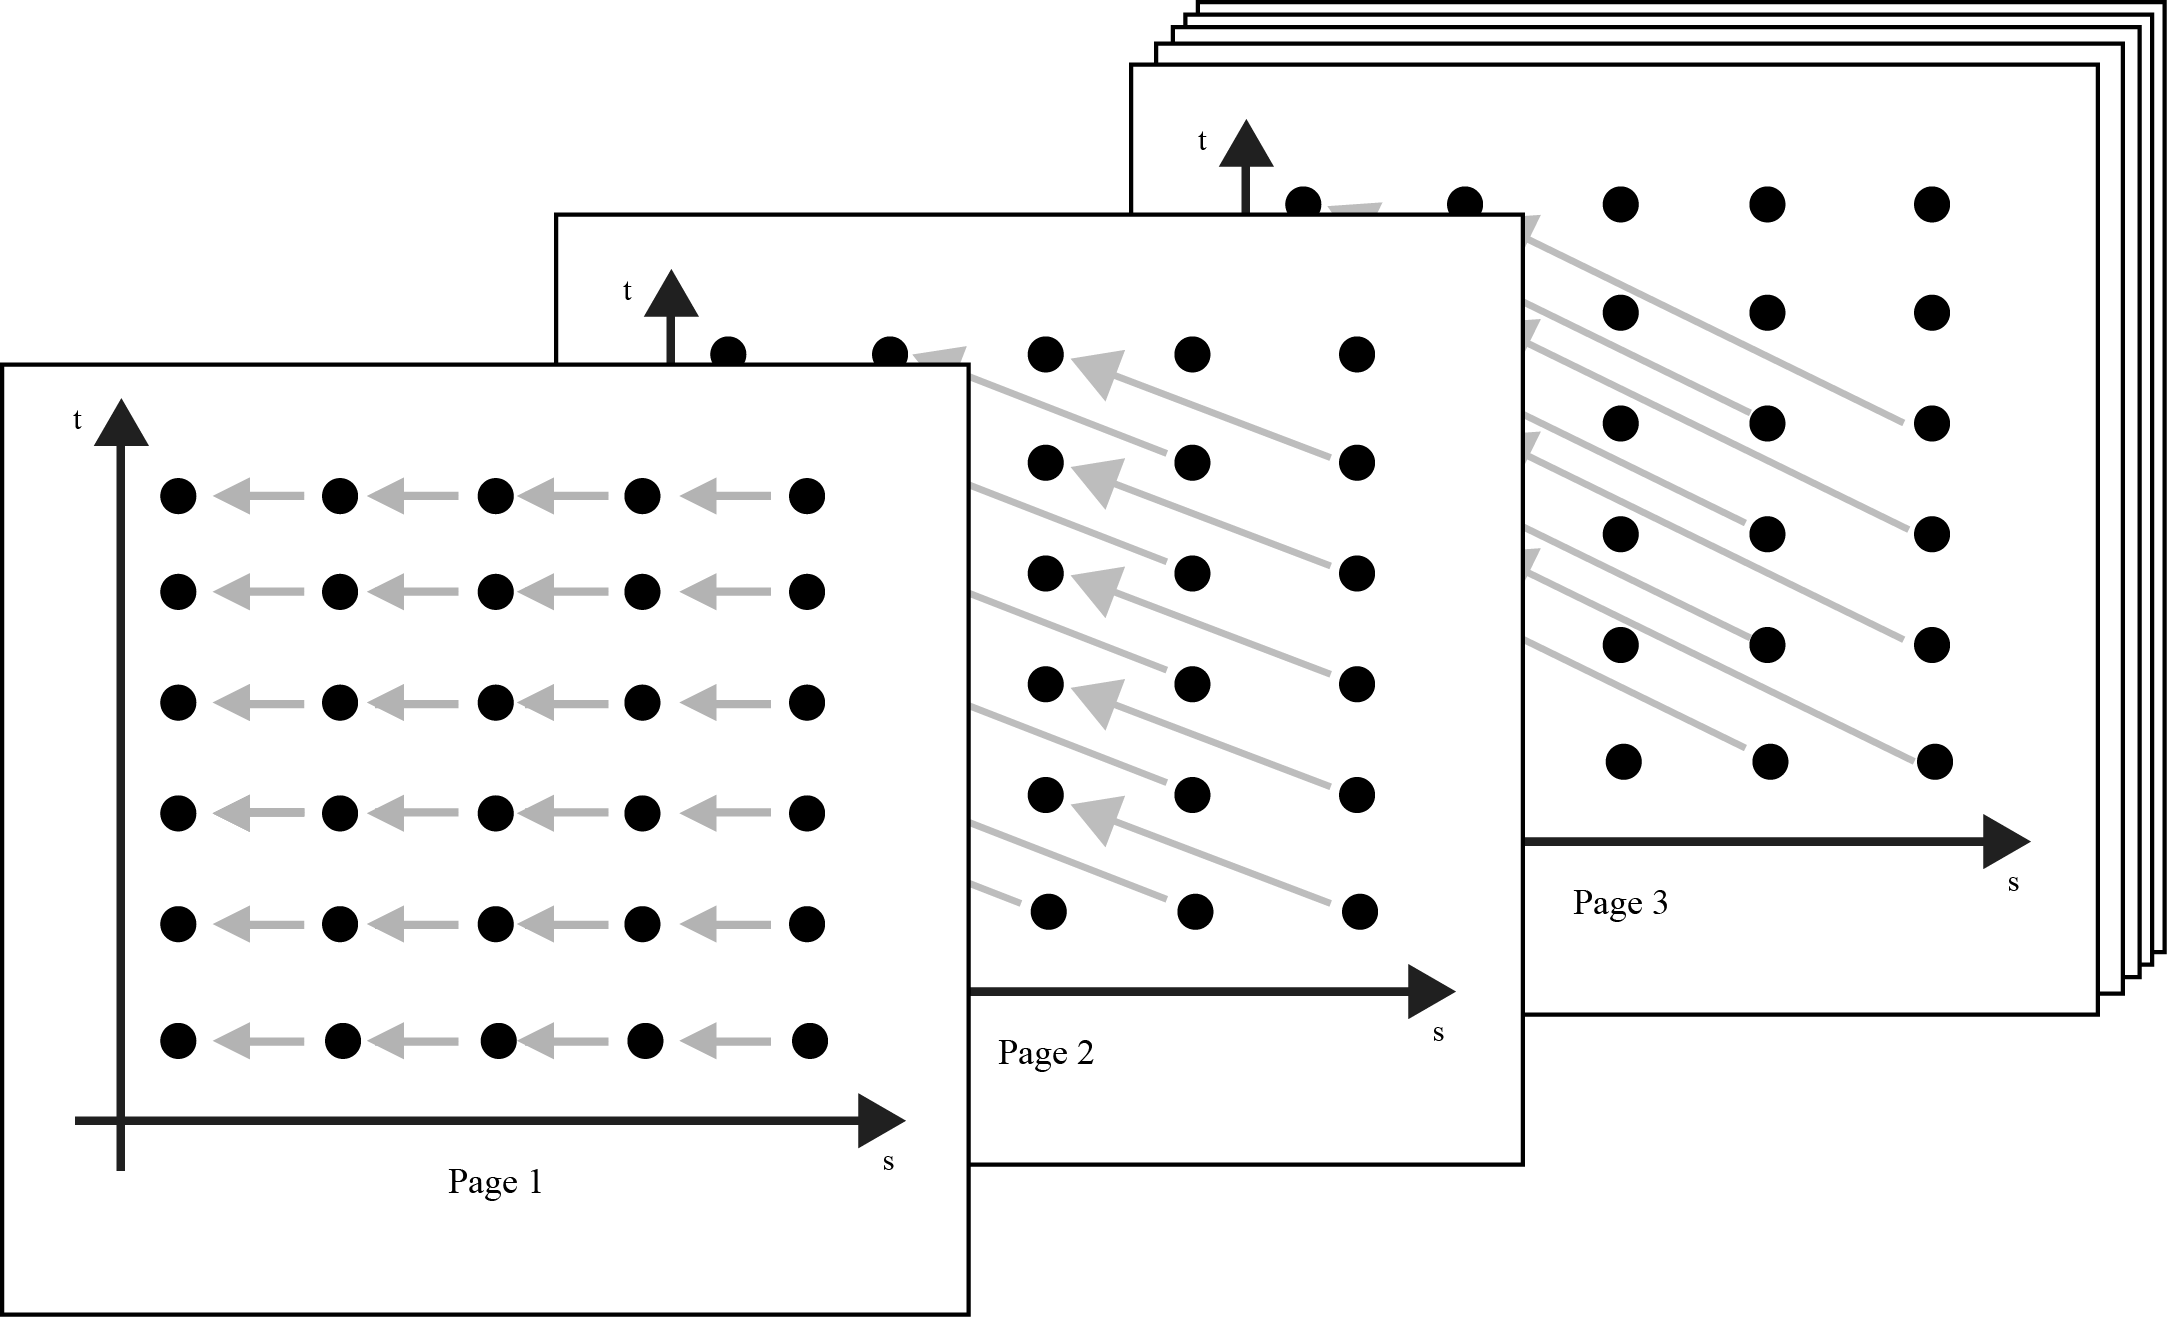
\includegraphics[width=\linewidth,height=0.45\textheight,keepaspectratio]{figures/cover.png}
  \end{center}
       \begin{minipage}{.35\linewidth}
    \begin{flushleft}
      \vspace{2em}
      {\fontsize{6pt}{2pt} \textit{Notes: These are notes live-tex'd
from a graduate course in Algebraic Geometry taught by Philip Engel at
the University of Georgia in Fall 2020. As such, any errors or
inaccuracies are almost certainly my own. } } \\
    \end{flushleft}
    \end{minipage}
    \hfill
    \begin{minipage}{.65\linewidth}
    \end{minipage}
  }







\begin{document}

\date{}
\author{D. Zack Garza}
\maketitle
\begin{flushleft}
\textit{D. Zack Garza} \\
\textit{University of Georgia} \\
  \textit{\href{mailto: dzackgarza@gmail.com}{dzackgarza@gmail.com}} \\
{\tiny \textit{Last updated:} 2020-12-14 }
\end{flushleft}


\newpage

\tableofcontents
\newpage

\hypertarget{prologue}{%
\section*{Prologue}\label{prologue}}
\addcontentsline{toc}{section}{Prologue}

\hypertarget{references}{%
\subsection{References}\label{references}}

\begin{itemize}
\tightlist
\item
  Gathmann's Algebraic Geometry notes\autocite{AndreasGathmann515}.
\end{itemize}

\hypertarget{notation}{%
\subsection{Notation}\label{notation}}

\begin{align*}  
V(I) && \text{The variety associated to an ideal } I \normal \kx{n}
.\end{align*}

\todo[inline]{Lots of notation to fill in.}

\newpage

\hypertarget{useful-algebra-facts}{%
\subsection{Useful Algebra Facts}\label{useful-algebra-facts}}

\begin{fact}

\envlist

\begin{itemize}
\tightlist
\item
  \(\mathfrak{p}\normal R\) is prime \(\iff R/\mathfrak{p}\) is a
  domain.
\item
  \(\mathfrak{p}\normal R\) is maximal \(\iff R/\mathfrak{p}\) is a
  field.
\item
  Maximal ideals are prime.
\item
  Prime ideals are radical.
\item
  If \(R\) is a PID and \(\gens{f} \normal R\) is generated by an
  irreducible element \(f\), then \(\gens{f}\) is maximal
\end{itemize}

\end{fact}

\begin{proposition}

A polynomial ring \(\kx{n}\) on finitely many generators is Noetherian.
In particular, every ideal \(I\normal \kx{n}\) has a finite set of
generators and can be written as \(I = \gens{f_1, \cdots, f_m}\).

\end{proposition}

\begin{proof}[?]

By Hilbert's basis theorem, every polynomial ring over a Noetherian ring
is again Noetherian. A field \(k\) is both Artinian and Noetherian,
since it has only two ideals and thus any chain of ideals necessarily
terminates.

\end{proof}

\begin{proposition}[Properties and Definitions of Ideal Operations]

\begin{align*}  
I+J   &\da \ts{f+g \st f\in I,\, g\in J} \\
IJ    &\da \ts{\sum_{i=1}^N f_i g_i \st f_i\in I,\, g_i\in J, N\in \NN} \\
I+J   = \gens{1} 
      &\implies I\intersect J = IJ && \text{(coprime or comaximal)}
\gens{a} + \gens{b} = \gens{a, b}
.\end{align*}

\end{proposition}

\begin{theorem}[Noether Normalization]\label{thm:noether_normalization}

Any finitely-generated field extension \(k_1 \injects k_2\) is a finite
extension of a purely transcendental extension, i.e.~there exist
\(t_1, \cdots, t_\ell\) such that \(k_2\) is finite over
\(k_1(t_1, \cdots, t_\ell)\).

\end{theorem}

\hypertarget{friday-august-21-intro-and-motivation}{%
\section{Friday, August 21: Intro and
Motivation}\label{friday-august-21-intro-and-motivation}}

\hypertarget{coordinate-rings}{%
\subsection{Coordinate Rings}\label{coordinate-rings}}

General idea: functions in a \emph{coordinate ring}
\(R[x_1, \cdots, x_n]/I\) will correspond to the geometry of the
\emph{variety} cut out by \(I\).

\begin{example}

\envlist

\begin{itemize}
\item
  \(x^2 + y^2 - 1\) defines a circle, say, over \(\RR\)
\item
  \(y^2 = x^3-x\) gives an elliptic curve:
\end{itemize}

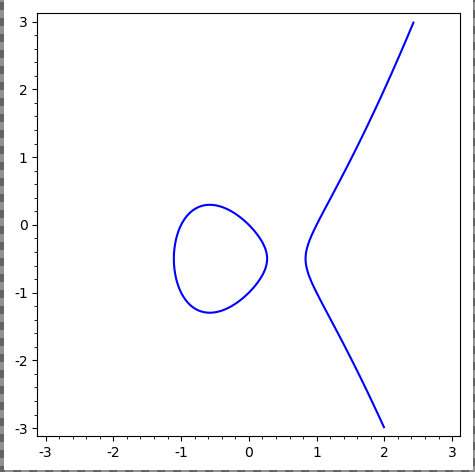
\includegraphics[width=3.64583in,height=\textheight]{figures/image_2020-08-21-01-04-22.png}

\begin{itemize}
\item
  \(x^n+y^n-1\): does it even contain a \(\QQ\dash\)point? (Fermat's
  Last Theorem)
\item
  \(x^2 + 1\), which has no \(\RR\dash\)points.
\item
  \(x^2 + y^2 + 1/\RR\) vanishes nowhere, so its ring of functions is
  not \(\RR[x, y] / \gens{x^2 + y^2 + 1}\). The problem: \(\RR\) is not
  algebraically closed.
\item
  \(x^2 - y^2 = 0\) over \(\CC\) is not a manifold (no chart at the
  origin):
\end{itemize}

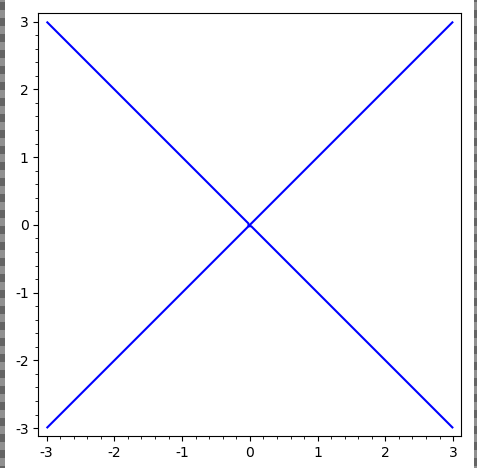
\includegraphics[width=3.64583in,height=\textheight]{figures/image_2020-08-21-01-23-32.png}

\begin{itemize}
\item
  \(x+y+1/\FF_3\), which has 3 points over \(\FF_3^2\), but
  \(f(x, y) = (x^3 - x)(y^3-y)\) vanishes at every point

  \begin{itemize}
  \item
    Not possible when algebraically closed (is there nonzero polynomial
    that vanishes on every point in \(\CC\)?)
  \item
    \(V(f) = \FF_3^2\), so the coordinate ring is zero instead of
    \(\FF_3[x, y]/\gens{f}\) (addressed by scheme theory)
  \end{itemize}
\end{itemize}

\end{example}

\hypertarget{harnack-curve-theorem}{%
\subsection{Harnack Curve Theorem}\label{harnack-curve-theorem}}

\begin{theorem}[Harnack Curve Theorem]

If \(f \in \RR[x, y]\) is of degree \(d\),
then{[}\^{}actual\_statement{]}
\begin{align*}  
\pi_1 V(f) \subseteq \RR^2 \leq 1 + {(d-1)(d-2) \over 2}
\end{align*} {[}\^{}actual\_statement{]}: Actual statement: the number
of connected components is bounded above by this quantity.

\end{theorem}

\begin{example}

Take the curve
\begin{align*}  
X = \theset{(x, y, z) = (t^3, t^4, t^5) \in \CC^3 \suchthat t\in \CC}
.\end{align*}

Then \(X\) is cut out by three equations:

\begin{itemize}
\tightlist
\item
  \(y^2 = xz\)
\item
  \(x^2 = yz\)
\item
  \(z^2 = x^2 y\)
\end{itemize}

\end{example}

\begin{exercise}

Show that the vanishing locus of the first two equations above is
\(X\union L\) for \(L\) a line.

\end{exercise}

Compare to linear algebra: codimension \(d\) iff cut out by exactly
\(d\) equations.

\hypertarget{connection-to-riemann-surfaces}{%
\subsection{Connection to Riemann
Surfaces}\label{connection-to-riemann-surfaces}}

\begin{example}

Given the Riemann surface
\begin{align*}  
y^2 = (x-1)(x-2)\cdots(x-2n)
,\end{align*} how does one visualize its solution set?

\end{example}

\begin{fact}

On \(\CC\) with some slits, you can consistently choose a square root of
the RHS.

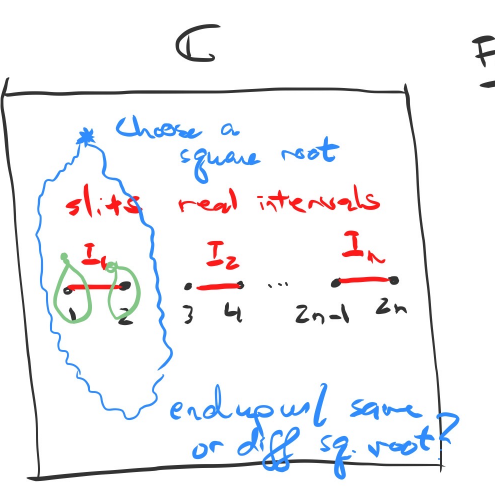
\includegraphics[width=3.64583in,height=\textheight]{figures/image_2020-08-21-01-31-47.png}

Away from \(x=1, \cdots, 2n\), there are two solutions for \(y\) given
\(x\).

After gluing along strips, obtain:

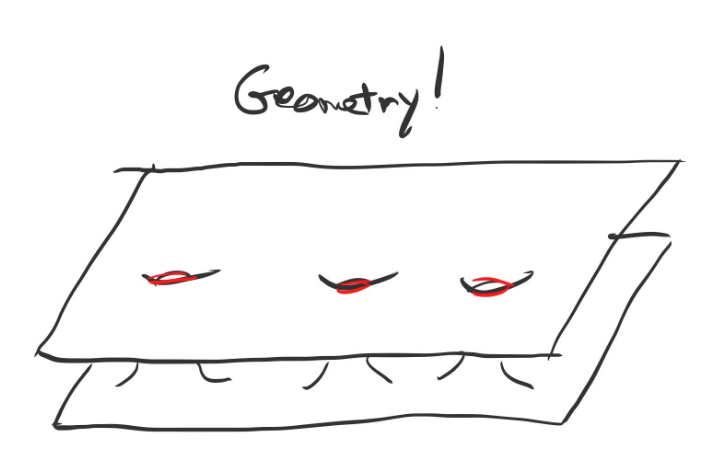
\includegraphics[width=3.64583in,height=\textheight]{figures/image_2020-08-21-01-32-48.png}

\end{fact}

\hypertarget{tuesday-august-25}{%
\section{Tuesday, August 25}\label{tuesday-august-25}}

\hypertarget{radicals-degrees-and-affine-varieties}{%
\subsection{Radicals, Degrees, and Affine
Varieties}\label{radicals-degrees-and-affine-varieties}}

Let \(k = \bar k\) and \(R\) a ring containing ideals \(I, J\). Recall
the definition of the \emph{radical}:

\begin{definition}[Radical]

The \emph{radical} of an ideal \(I \normal R\) is defined as
\begin{align*}  
\sqrt{I} = \ts{r\in R \st r^k\in I \text{ for some } k\in \NN}
.\end{align*}

\end{definition}

\begin{example}

Let
\begin{align*}
I &= (x_1, x_2^2) \subset \CC[x_1, x_2] \\
  &= \ts{ f_1 x_1 + f_2 x_2 \st f_1, f_2 \in \CC[x_1, x_2]}
\end{align*}

Then \(\sqrt{I} = (x_1, x_2)\), since
\(x_2^2 \in I \implies x_2 \in \sqrt{I}\).

\end{example}

Given \(f\in k[x_1, \cdots, x_n]\), take its value at
\(a = (a_1, \cdots, a_n)\) and denote it \(f(a)\).

\begin{definition}[Degree of an element of $\kxn$]

Define \(\deg(f)\) as the largest value of \(i_1 + \cdots + i_n\) such
that the coefficient of \(\prod x_j ^{i_j}\) is nonzero.

\end{definition}

\begin{example}

\(\deg(x_1 + x_2^2 + x_1 x_2^3) = 4\)

\end{example}

\begin{definition}[Affine Variety]

\envlist

\begin{enumerate}
\def\labelenumi{\arabic{enumi}.}
\item
  Affine \(n\dash\)space \(\AA^n = \AA_k^n\) is defined as
  \(\theset{(a_1, \cdots, a_n) \suchthat a_i \in k}\).\footnote{Not
    \(k^n\), since we won't necessarily use the vector space structure
    (e.g.~adding points).}
\item
  Let \(S\subset k[x_1, \cdots, x_n]\) be a \textbf{set} of
  polynomials.\footnote{We don't necessarily require \(S\) to be an
    ideal in this definition. We will shortly show that taking the ideal
    it generates yields the same variety.}
\end{enumerate}

Then define the \textbf{affine variety} of \(S\) as
\begin{align*}
  V(S) \da \ts{x\in \AA^n \st f(x) = 0} \subset \AA^n
  \end{align*}

\end{definition}

\begin{example}[Examples of affine varieties]

\envlist

\begin{itemize}
\tightlist
\item
  Let \(f(x) = 0\), then \(\AA^n = V\qty{\ts{f}}\) is an affine variety.
\item
  Any point \((a_1, \cdots, a_n)\in \AA^n\) is an affine variety,
  uniquely determined by
  \(V(x_1 - a_1, \cdots, x_n - a_n) = \theset{a_1, \cdots, a_n}\).
\item
  For any finite set \(r_1, \cdots, r_k \in \AA^1\), there exists a
  polynomial \(f\in k[x_1]\) whose roots are \(r_i\).
\end{itemize}

\end{example}

\begin{remark}

We may as well assume \(S\) is an ideal by taking the ideal it
generates,
\begin{align*}
S\subseteq \gens{S} = \ts{\sum g_i f_i \suchthat g_i \in k[x_1, \cdots, x_n],\, f_i\in S}
.\end{align*}

\begin{claim}

\begin{align*}  
V(S) = V\qty{\gens{S}}
.\end{align*}

\end{claim}

It's clear that \(V(\gens{S}) \subset V(S)\).

Conversely, if \(f_1, f_2\) vanish at \(x\in \AA^n\), then \(f_1 + f_2\)
and \(gf_1\) also vanish at \(x\) for all \(g\in k[x_1, \cdots, x_n]\).
Thus \(V(S) \subset V(\gens{S})\).

\end{remark}

\hypertarget{ideals-and-properties-of-vwait}{%
\subsection{\texorpdfstring{Ideals, and Properties of
\(V(\wait)\)}{Ideals, and Properties of V(\textbackslash wait)}}\label{ideals-and-properties-of-vwait}}

See \cref{useful-algebra-facts} for a review of properties of ideals.

\begin{proposition}[Properties of $V$]

\envlist

\begin{enumerate}
\def\labelenumi{\arabic{enumi}.}
\tightlist
\item
  If \(S_1 \subseteq S_2\) then \(V(S_1) \supseteq V(S_2)\).
\item
  \(V(S_1) \union V(S_2) = V(S_1 S_2) = V(S_1 \intersect S_2)\).
\item
  \(\bigcap V(S_i) = V\qty{\bigcup S_i}\).
\end{enumerate}

\end{proposition}

We thus have a map
\begin{align*}  
V: \ts{\text{Ideals in } k[x_1, \cdots, x_n]} \to \ts{\text{Affine varieties in } \AA^n}
.\end{align*}

\begin{definition}[The Ideal of a Set]

Let \(X\subset \AA^n\) be any set, then \emph{the ideal of \(X\)} is
defined as
\begin{align*}  
I(X) \da\ts{f\in k[x_1, \cdots, x_n] \st f(x) = 0\, \forall x\in X}
.\end{align*}

\end{definition}

\begin{example}

Let \(X\) be the union of the \(x_1\) and \(x_2\) axes in \(\AA^2\),
then
\begin{align*}
I(X) = \gens{x_1 x_2} = \ts {g x_1 x_2 \st g\in k[x_1, x_2]}
.\end{align*}

\end{example}

\begin{proposition}[$I$ is inclusion-reversing]

If \(X_1 \subset X_2\) then \(I(X_1) \supset I(X_2)\).

\end{proposition}

\begin{proof}[?]

If \(f\in I(X_2)\), then \(f(x) = 0\) for all \(x\in X_2\). Since
\(X_1 \subset X_2\), we have \(f(x) = 0\) for all \(x\in X_1\), so
\(f\in I(X_2)\).

\end{proof}

\begin{proposition}[The Image of $V$ is Radical]

\(I(X)\) is a radical ideal, i.e.~\(I(X) = \sqrt{I(X)}\).

\end{proposition}

\begin{proof}[?]

If \(f(x)^k = 0\) for all \(x\in X\), then \(f(x) = 0\) for all
\(x\in X\). Then \(f^k \in I(X)\) and thus \(f\in I(X)\).

\end{proof}

These maps thus yield correspondences
\begin{align*}  
\correspond{\text{Ideals in } k[x_1, \cdots, x_n]} &\mapsvia{V} \correspond{\text{Affine Varieties}} \\
\correspond{\text{Radical Ideals}} &\fromvia{I} \correspond{\text{Affine Varieties}}
.\end{align*}

We'll find that if we restrict to radical ideals, this will yield a
bijective correspondence.

\hypertarget{statement-and-proof-of-nullstellensatz}{%
\subsection{Statement and Proof of
Nullstellensatz}\label{statement-and-proof-of-nullstellensatz}}

\begin{theorem}[Hilbert Nullstellensatz (Zero Locus Theorem)]

\envlist

\begin{enumerate}
\def\labelenumi{\alph{enumi}.}
\item
  For any affine variety \(X\),
  \begin{align*}
  V(I(X)) = X
  .\end{align*}
\item
  For any ideal \(J \subset k[x_1, \cdots, x_n]\),
  \begin{align*}
  I(V(J)) = \sqrt{J}
  .\end{align*}
\end{enumerate}

Thus there is a bijection between radical ideals and affine varieties.

\end{theorem}

\begin{fact}

Recall the Hilbert Basis Theorem: any ideal in a finitely generated
polynomial ring over a field is again finitely generated.

\end{fact}

We need to show 4 inclusions, 3 of which are easy.

\begin{proof}[of the easy inclusions]

\envlist

\begin{enumerate}
\def\labelenumi{\alph{enumi}.}
\tightlist
\item
  \(X \subset V(I(X))\):
\end{enumerate}

\begin{itemize}
\tightlist
\item
  If \(x\in X\) then \(f(x) = 0\) for all \(f\in I(X)\).
\item
  So \(x\in V(I(X))\), since every \(f\in I(X)\) vanishes at \(x\).
\end{itemize}

\begin{enumerate}
\def\labelenumi{\alph{enumi}.}
\setcounter{enumi}{1}
\tightlist
\item
  \(\sqrt{J} \subset I(V(J))\):
\end{enumerate}

\begin{itemize}
\tightlist
\item
  If \(f\in \sqrt{J}\) then \(f^k \in J\) for some \(k\).
\item
  Then \(f^k(x) = 0\) for all \(x\in V(J)\).
\item
  So \(f(x) = 0\) for all \(x\in V(J)\).
\item
  Thus \(f\in I(V(J))\).
\end{itemize}

\begin{enumerate}
\def\labelenumi{\alph{enumi}.}
\setcounter{enumi}{2}
\tightlist
\item
  \(V(I(X)) \subset X\):
\end{enumerate}

\begin{itemize}
\tightlist
\item
  Need to now use that \(X\) is an affine variety.

  \begin{itemize}
  \tightlist
  \item
    Counterexample: \(X = \ZZ^2 \subset \CC^2\), then \(I(X) = 0\). But
    \(V(I(X)) = \CC^2 \not\subset \ZZ^2\).
  \end{itemize}
\item
  By (b), \(I(V(J)) \supset \sqrt{J} \supset J\).
\item
  Since \(V(\wait)\) is order-reversing, taking \(V\) of both sides
  reverses the containment.
\item
  So \(V(I(V(J))) \subset V(J)\), i.e.~\(V(I(X)) \subset X\).
\end{itemize}

\end{proof}

Thus the hard direction that remains is (d),

\begin{align*}
I(V(J)) \subset \sqrt{J}
\end{align*}

We'll need Noether Normalization, which is stated in
\cref{thm:noether_normalization}.

\begin{warnings}

Noether normalization is perhaps more important than the
Nullstellensatz!

\end{warnings}

\begin{theorem}[1st Version of Nullstellensatz]

Suppose \(k\) is algebraically closed and uncountable \footnote{Still
  true in countable case by a different proof.} Then the maximal ideals
in \(k[x_1, \cdots, x_n]\) are of the form
\((x_1 - a_1, \cdots, x_n - a_n)\).

\end{theorem}

\begin{proof}

Let \(\mfm\) be a maximal ideal, then by the Hilbert Basis Theorem,
\(\mfm = \gens{f_1, \cdots, f_r}\) is finitely generated. Let
\(L = \QQ[\ts {c_i}]\) where the \(c_i\) are all of the coefficients of
the \(f_i\) if \(\ch(K) = 0\), \textbf{or} \(\FF_p[\ts {c_i}]\) if
\(\ch(k) = p\). Then \(L\subset k\). Define
\(\mfm_0 = \mfm\intersect L[x_1, \cdots, x_n]\). Note that by
construction, \(f_i \in \mfm_0\) for all \(i\), and we can write
\(\mfm = \mfm_0 \cdot k[x_1, \cdots, x_n]\).

\begin{claim}

\(\mfm_0\) is a maximal ideal.

\end{claim}

If it were the case that
\begin{align*}  
\mfm_0 \subsetneq \mfm_0' \subsetneq L[x_1, \cdots, x_n]
,\end{align*} then
\begin{align*}  
\mfm_0\cdot k[x_1, \cdots, x_n] \subsetneq \mfm_0'\cdot k[x_1, \cdots, x_n]  \subsetneq k[x_1, \cdots, x_n]
.\end{align*}

So far, we've constructed a smaller polynomial ring and a maximal ideal
in it. Thus \(L[x_1, \cdots, x_n]/\mfm_0\) is a field that is finitely
generated over either \(\QQ\) or \(\FF_p\). So
\(L[x_1, \cdots, x_n]/\mfm_0\) is finite over some
\(\QQ(t_1, \cdots, t_n)\), and since \(k\) is uncountable, there exists
an embedding \(\QQ(t_1, \cdots, t_n) \injects k\).\footnote{Here we use
  the fact that there are only countably many polynomials over a
  countable field.}\\

This extends to an embedding of
\(\phi: L[x_1, \cdots, x_n]/\mfm_0 \injects k\) since \(k\) is
algebraically closed. Letting \(a_i\) be the image of \(x_i\) under
\(\phi\), then \(f(a_1, \cdots, a_n) = 0\) by construction,
\(f_i \in (x_i - a_i)\) implies that \(\mfm = (x_i - a_i)\) by
maximality.

\end{proof}

\hypertarget{thursday-august-27}{%
\section{Thursday, August 27}\label{thursday-august-27}}

\hypertarget{consequence-of-the-nullstellensatz}{%
\subsection{Consequence of the
Nullstellensatz}\label{consequence-of-the-nullstellensatz}}

Recall Hilbert's Nullstellensatz:

\begin{enumerate}
\def\labelenumi{\alph{enumi}.}
\item
  For any affine variety, \(V(I(X)) = X\).
\item
  For any ideal \(J\normal k[x_1, \cdots, x_n]\),
  \(I(V(J)) = \sqrt{J}\).
\end{enumerate}

So there's an order-reversing bijection
\begin{align*}  
\correspond{\text{Radical ideals } k[x_1, \cdots, x_n]} \to{V(\wait)}{I(\wait)}
\correspond{\text{Affine varieties in } \AA^n}
.\end{align*}

In proving \(I(V(J)) \subseteq \sqrt{J}\), we had an important lemma
(Noether Normalization): the maximal ideals of \(k[x_1, \cdots, x_n]\)
are of the form \(\gens{x-a_1, \cdots, x-a_n}\).

\begin{corollary}[?]

If \(V(I)\) is empty, then \(I = \gens{1}\).

\end{corollary}

\begin{remark}

This is because no common vanishing locus \(\implies\) trivial ideal, so
there's a linear combination that equals 1.

\end{remark}

\begin{slogan}

The only ideals that vanish nowhere are trivial.

\end{slogan}

\begin{proof}

By contrapositive, suppose \(I\neq \gens{1}\). By Zorn's Lemma, these
exists a maximal ideals \(\mfm\) such that \(I \subset \mfm\). By the
order-reversing property of \(V(\wait)\), \(V(\mfm) \subseteq V(I)\). By
the classification of maximal ideals,
\(\mfm = \gens{x-a_1, \cdots, x-a_n}\), so
\(V(\mfm) = \theset{a_1, \cdots, a_n}\) is nonempty.

\end{proof}

\hypertarget{proof-of-remaining-part-of-nullstellensatz}{%
\subsection{Proof of Remaining Part of
Nullstellensatz}\label{proof-of-remaining-part-of-nullstellensatz}}

We now return to the remaining hard part of the proof of the
Nullstellensatz:

\begin{align*}
I(V(J)) \subseteq \sqrt{J}
\end{align*}

Let \(f\in V(I(J))\), we want to show \(f\in \sqrt{J}\). Consider the
ideal
\begin{align*}
\tilde J \da J + \gens{ft - 1} \subseteq k[x_1, \cdots, x_n, t]
\end{align*}

\begin{observation}

\(f = 0\) on all of \(V(J)\) by the definition of \(I(V(J))\).

\end{observation}

However, if \(f=0\), then \(ft-1 \neq 0\), so
\begin{align*}
V(\tilde J) = V(G) \intersect V(ft-1) = \emptyset
\end{align*}

\begin{figure}
\centering
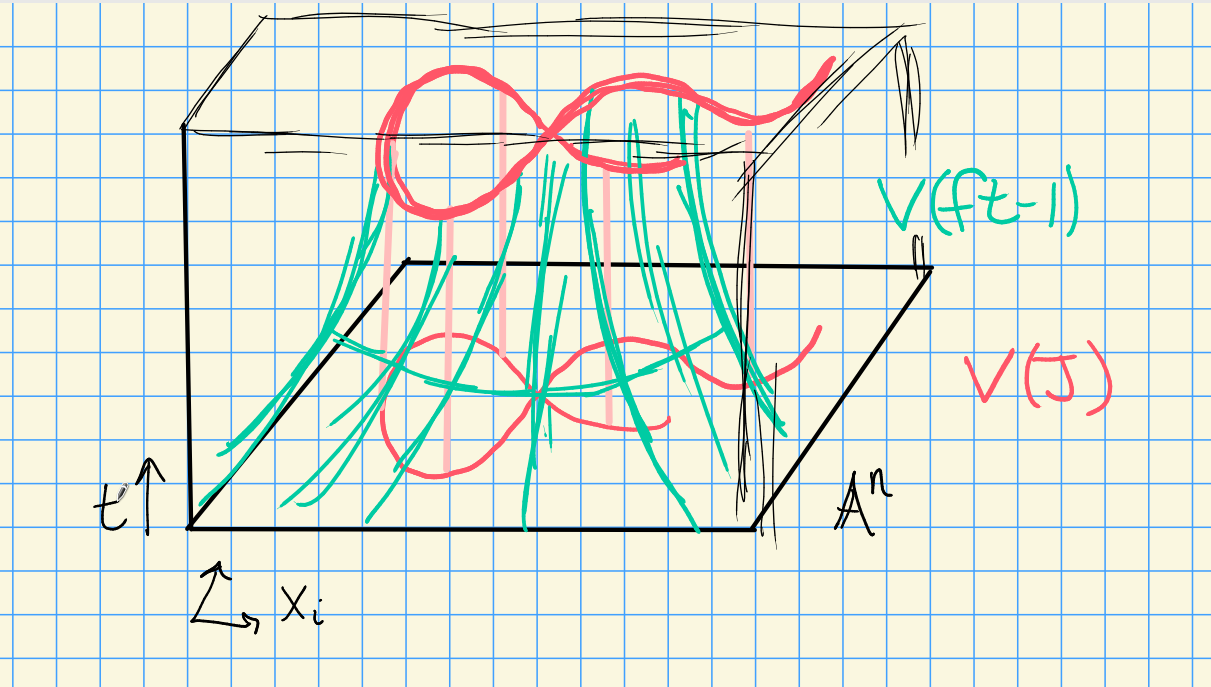
\includegraphics[width=3.64583in,height=\textheight]{figures/image_2020-08-27-09-56-33.png}
\caption{Effect, a hyperbolic tube around \(V(J)\), so both can't
vanish}
\end{figure}

Applying the corollary \(\tilde J = (1)\), so
\begin{align*}
1 = \gens{ft-1} g_0(x_1, \cdots, x_n, t) + \sum f_i g_i(x_1, \cdots, x_n, t)
\end{align*} with \(f_i \in J\). Let \(t^N\) be the largest power of
\(t\) in any \(g_i\). Thus for some polynomials \(G_i\), we have
\begin{align*}  
f^N \da (ft-1) G_0(x_1, \cdots, x_n, ft) + \sum f_i G_i(x_1, \cdots, x_n, ft)
\end{align*} noting that \(f\) does not depend on \(t\). Now take
\(k[x_1, \cdots, x_n, t]/\gens{ft-1}\), so \(ft=1\) in this ring. This
kills the first term above, yielding
\begin{align*}  
f^N = \sum f_i G_i(x_1, \cdots, x_n, 1) \in k[x_1, \cdots, x_n, t]/\gens{ft-1}
.\end{align*}

\begin{proposition}[?]\label{prop:inclusion_of_stuff}

There is an inclusion
\begin{align*}  
k[x_1, \cdots, x_n] \injects
k[x_1, \cdots, x_n, t]/\gens{ft-1}
.\end{align*}

\end{proposition}

Since this is injective, this identity also holds in
\(k[x_1, \cdots, x_n]\). But \(f_i\in J\), so \(f\in \sqrt{I}\).

\(\qed\)

\begin{exercise}[?]

Why is this true? See \cref{prop:inclusion_of_stuff}.

\end{exercise}

\begin{example}

Consider \(k[x]\). If \(J\subset k[x]\) is an ideal, it is principal, so
\(J = \gens{f}\). We can factor \(f(x) = \prod_{i=1}^k (x-a_i)^{n_i}\)
and \(V(f) = \ts{a_1, \cdots, a_k}\). Then
\begin{align*}
I(V(f)) = \gens{(x-a_1)(x-a_2)\cdots(x-a_k)} = \sqrt{J} \subsetneq J
,\end{align*} so this loses information.

\end{example}

\begin{example}

Let \(J = \gens{x-a_1, \cdots, x-a_n}\), then \(I(V(J)) = \sqrt{J} = J\)
with \(J\) maximal. Thus there is a correspondence
\begin{align*}  
\correspond{\text{Points of } \AA^n} \iff 
\correspond{\text{Maximal ideals of }k[x_1, \cdots, x_n]}
.\end{align*}

\end{example}

\begin{theorem}[Properties of $I$]

\envlist

\begin{enumerate}
\def\labelenumi{\alph{enumi}.}
\item
  \(I(X_1 \union X_2) = I(X_1) \intersect I(X_2)\).
\item
  \(I(X_1) \intersect I(X_2) = \sqrt{I(X_1) + I(X_2)}\).
\end{enumerate}

\end{theorem}

\begin{proof}

We proved (a) on the variety side.

For (b), by the Nullstellensatz, \(X_i = V(I(X_i))\), so
\begin{align*}  
I(X_1\intersect X_2) 
&=
I\qty{ VI(X_1) \intersect VI(X_2)} \\
&=
IV\qty{I(X_1) + I(X_2)} \\
&= \sqrt{I(X_1) + I(X_2)}
.\end{align*}

\end{proof}

\begin{example}

Example of property (b):

Take \(X_1 = V(y-x^2)\) and \(X_2 = V(y)\), a parabola and the
\(x\dash\)axis.

\begin{figure}
\centering
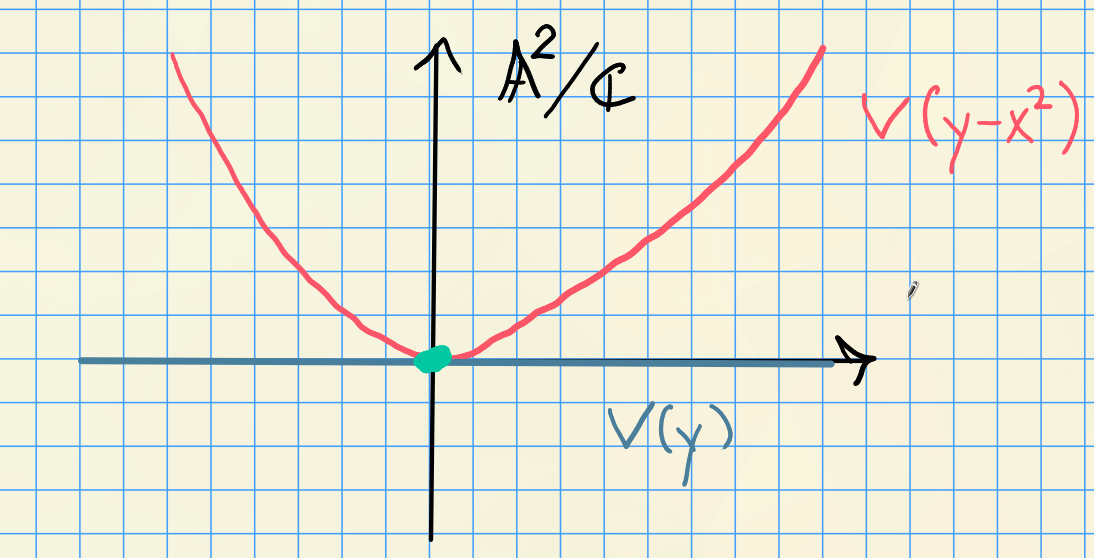
\includegraphics[width=3.64583in,height=\textheight]{figures/image_2020-08-27-10-26-45.png}
\caption{Intersecting \(V(y-x^2)\) and \(V(y)\)}
\end{figure}

Then \(X_1 \intersect X_2 = \ts{(0, 0)}\), and
\(I(X_1) + I(X_2) = \gens{y-x^2, y} = \gens{x^2, y}\), but
\begin{align*}
I(X_1 \intersect X_2) = \gens{x, y} = \sqrt{\gens{x^2, y}}
\end{align*}

\end{example}

\begin{proposition}[?]

If \(f, g\in k[x_1, \cdots, x_n]\), and suppose \(f(x) = g(x)\) for all
\(x\in \AA^n\). Then \(f = g\).

\end{proposition}

\begin{proof}

Since \(f-g\) vanishes everywhere,
\(f-g \in I(\AA^n) = I(V(0)) = \sqrt{0} = 0\).

\end{proof}

More generally suppose \(f(x) = g(x)\) for all \(x\in X\), where \(X\)
is some affine variety. Then by definition, \(f-g \in I(X)\), so a
``natural'' space of functions on \(X\) is \(k[x_1,\cdots, x_n]/I(X)\).

\begin{definition}[Coordinate Ring]

For an affine variety \(X\), the \emph{coordinate ring of \(X\)} is
\begin{align*}  
A(X) \da k[x_1, \cdots, x_n]/ I(X)
.\end{align*}

Elements \(f\in A(X)\) are called \emph{polynomial} or \emph{regular}
functions on \(X\).

\end{definition}

\begin{observation}

The constructions \(V(\wait), I(\wait)\) work just as well for \(A(X)\)
and \(X\).

\end{observation}

Given any \(S\subset A(Y)\) for \(Y\) an affine variety,
\begin{align*}  
V(S) = V_Y(S) \da\ts{x\in Y \st f(x) = 0\,\,\forall f\in S}
.\end{align*}

Given \(X\subset Y\) a subset,
\begin{align*}  
I(X) = I_Y(X) \da\ts{f\in A(Y) \st f(x) = 0\,\,\forall x\in X} \subseteq A(Y)
.\end{align*}

\begin{example}

For \(X\subset Y \subset \AA^n\), we have
\(I(X) \supset I(Y) \supset I(\AA^n)\), so we have maps

\begin{center}
\begin{tikzcd}
A(\AA^n) \ar[rr, twoheadrightarrow, "\wait/I(X)", bend left] \ar[r, "\wait/I(Y)", twoheadrightarrow] &A(Y)\ar[r, twoheadrightarrow, "\wait/I(X)"] &A(X) \\
\end{tikzcd}
\end{center}

\end{example}

\begin{theorem}[?]

Let \(X\subset Y\) be an affine subvariety, then

\begin{enumerate}
\def\labelenumi{\alph{enumi}.}
\item
  \(A(X) = A(Y) / I_Y(X)\)
\item
  There is a correspondence
  \begin{align*}  
  \correspond{\text{Affine subvarieties of }Y} 
  &\iff \correspond{\text{Radical ideals in }A(Y)} \\
  X &\mapsto I_Y(X) \\
  V_Y(J) &\mapsfrom J
  .\end{align*}
\end{enumerate}

\end{theorem}

\begin{proof}

Properties are inherited from the case of \(\AA^n\), see exercise in
Gathmann.

\end{proof}

\begin{example}

Let \(Y = V(y-x^2) \subset \AA^2/\CC\) and
\(X = \ts{(1, 1)} = V(x-1, y-1)\subset \AA^2/\CC\).

Then there is an inclusion \(\gens{y-x^2} \subset \gens{x-1, y-1}\)
(e.g.~by Taylor expanding about the point \((1, 1)\)), and there is a
map

\begin{center}
\begin{tikzcd}
A(\AA^n)\ar[r]\ar[d, equal] & A(Y) \ar[r]\ar[d, equal] & A(X)\ar[d, equal] \\
k[x, y]\ar[r] & k[x, y]/\gens{y-x^2}\ar[r] & k[x, y]/\gens{x-1, y-1}
\end{tikzcd}
\end{center}

\end{example}

\hypertarget{tuesday-september-01}{%
\section{Tuesday, September 01}\label{tuesday-september-01}}

Last time: \(V(I) = \ts{x\in \AA^n \st f(x) = 0 \, \forall x\in I}\) and
\(I(X) = \ts{f\in k[x_1, \cdots, x_n] \st f(x) = 0\, \forall x\in X}\).
We proved the Hilbert Nullstellensatz \(I(V(J)) = \sqrt{J}\), defined
the coordinate ring of an affine variety \(X\) as
\(A(X) \da k[x_1, \cdots, x_n] / I(X)\), the ring of ``regular''
(polynomial) functions on \(X\).

Recall that a \emph{topology} on \(X\) can be defined as a collection of
``closed'' subsets of \(X\) that are closed under arbitrary
intersections and finite unions. A subset \(Y\subset X\) inherits a
subspace topology with closed sets of the form \(Z\intersect Y\) for
\(Z\subset X\) closed.

\begin{definition}[Zariski Topology]

Let \(X\) be an affine variety. The closed sets are affine subvarieties
\(Y\subset X\).

\end{definition}

We have \(\emptyset, X\) closed, since

\begin{enumerate}
\def\labelenumi{\arabic{enumi}.}
\tightlist
\item
  \(V_X(1) = \emptyset\),
\item
  \(V_X(0) = X\)
\end{enumerate}

Closure under finite unions: Let \(V_X(I), V_X(J)\) be closed in \(X\)
with \(I, J \subset A(X)\) ideals. Then
\(V_X(IJ) = V_X(I) \union V_X(J)\).

Closure under intersections: We have
\(\bigcap_{i\in \sigma} V_X(J) = V_X\qty{ \sum_{i\in \sigma} J_i}\).

\begin{remark}

There are few closed sets, so this is a ``weak'' topology.

\end{remark}

\begin{example}

Compare the classical topology on \(\AA^1/\CC\) to the Zariski topology.

Consider the set \(A\da \ts{x\in \AA^1/\CC \st \norm{x} \leq 1}\), which
is closed in the classical topology.

But \(A\) is not closed in the Zariski topology, since the closed
subsets are finite sets or the whole space.

\begin{quote}
Here the topology is in fact the cofinite topology.
\end{quote}

\end{example}

\begin{example}

Let \(f: \AA^1/k\to \AA^1/k\) be any injective map. Then \(f\) is
necessarily continuous wrt the Zariski topology.

\end{example}

Thus the notion of continuity is too weak in this situation.

\begin{example}

Consider \(X\cross Y\) a product of affine varieties. Then there is a
product topology where open sets are of the form
\(\bigcup_{i=1}^n U_i \cross V_i\) with \(U_i, V_i\) open in \(X, Y\)
respectively.

This is the wrong topology! On \(\AA^1 \cross \AA^1 = \AA^2\), the
diagonal \(\Delta \da V(x-y)\) is closed in the Zariski topology on
\(\AA^2\) but not in the product topology.

\end{example}

\begin{example}

Consider \(\AA^2/\CC\), so the closed sets are curves and points.
Observation: \(V(x_1 x_2 ) \subset \AA^2/\CC\) decomposed into the union
of the coordinate axes \(X_1 \da V(x_1)\) and \(X_2 \da V(x_2)\). The
Zariski topology can detect these decompositions.

\end{example}

\begin{definition}[Irreducibility and Connectedness]

Let \(X\) be a topological space.

\begin{enumerate}
\def\labelenumi{\alph{enumi}.}
\item
  \(X\) is \emph{reducible} iff there exist nonempty proper closed
  subsets \(X_1 ,X_2 \subset X\) such that \(X = X_1 \union X_2\).
  Otherwise, \(X\) is said to be \emph{irreducible}.
\item
  \(X\) is \emph{disconnected} if there exist \(X_1, X_2 \subset X\)
  such that \(X = X_1 \disjoint X_2\). Otherwise, \(X\) is said to be
  \emph{connected}.
\end{enumerate}

\end{definition}

\begin{example}

\(V(x_1 x_2)\) is reducible but connected.

\end{example}

\begin{remark}

\(\AA^1/\CC\) is \emph{not} irreducible, since we can write
\(\AA^1/\CC = \ts{\norm{x} \leq 1} \union \ts{\norm{x} \geq 1}\).

\end{remark}

\begin{proposition}[?]

Let \(X\) be a disconnected affine variety with
\(X = X_1 \disjoint X_2\). Then \(A(X) \cong A(X_1) \cross A(X_2)\).

\end{proposition}

\begin{proof}

We have \(X_1 \union X_2 = X\), so
\(I(X_1) \intersect I(X_2) = I(X) = (0)\) in the coordinate ring
\(A(X)\) (recalling that it is a quotient by \(I(X)\).)

Since \(X_1 \intersect X_1 \emptyset\), we have
\begin{align*}  
I(X_1 \intersect X_2) = \sqrt{I(X_1) + I(X_2) } = I(\emptyset) = \gens{1}
.\end{align*}

Thus \(I(X_1) + I(X_2) = \gens{1}\), and by the Chinese Remainder
Theorem, the following map is an isomorphism:
\begin{align*}  
A(X) \to A(X)/I(X_1) \cross A(X) / I(X_2)
.\end{align*}

But the codomain is precisely \(A(X_1) \cross A(X_2)\).

\end{proof}

\begin{proposition}[?]

An affine variety \(X\) is irreducible \(\iff\) \(A(X)\) is an integral
domain.

\end{proposition}

\begin{proof}

\(\implies\): By contrapositive, suppose \(f_1, f_2 \in A(X)\) are
nonzero with \(f_1 f_2 = 0\). Let \(X_i = V(f_i)\), then
\(X= V(0) = V(f_1 f_2) = X_1 \union X_2\) which are closed and proper
since \(f_i \neq 0\).

\hfill\break

\(\impliedby\): Suppose \(X\) is reducible with \(X = X_1 \union X_2\)
with \(X_i\) proper and closed. Define \(J_i \da I(X_i)\), and note
\(J_i \neq 0\) because \(V(J_i) = V(I(X_i)) = X_i\) by part (a) of the
Nullstellensatz.

So there exists a nonzero \(f_i \in J_i = I(X_i)\), so \(f_i\) vanishes
on \(X_i\). But then
\(V(f_1) \union V(f_2) \supset X_1 \union X_2 = X\), so
\(X= V(f_1 f_2)\) and \(f_1 f_2 \in I(X) = \gens{0}\) and
\(f_1 f_2 = 0\). So \(A(X)\) is not a domain.

\end{proof}

\begin{example}

Let \(X = \ts{p_1, \cdots, p_d}\) be a finite set in \(\AA^n\). The
Zariski topology on \(X\) is the discrete topology, and
\(X = \disjoint \ts{p_i}\). So
\begin{align*}  
A(X) = A(\disjoint \ts{p_i}) = \prod_{i=1}^d A({\ts{p_i}}) = \prod_{i=1}^d k[x_1, \cdots, x_n] / \gens{x_j - a_j(p_i)}_{j=1}^d
.\end{align*}

\end{example}

\begin{example}

Set \(V(x_1 x_2) = X\), then \(A(X) = k[x_1, x_2]/ \gens{x_1 x_2}\).
This not being a domain (since \(x_1 x_2 = 0\)) corresponds to
\(X = V(x_1) \union V(x_2)\) not being irreducible.

\end{example}

\begin{example}

\(\AA^2/k\) is irreducible since \(k[x_1, \cdots x_n]\) is a domain.

\end{example}

\begin{example}

Let \(X_1\) be the \(xy\) plane and \(X_2\) be the line parallel to the
\(y\dash\)axis through \(\thevector{0,0,1}\), and let
\(X= X_1 \disjoint X_2\). Then \(X_1 = V(z)\) and \(X_2 = V(x, z-1)\),
and \(I(X) = \gens{z} \cdots \gens{x, z-1}= \gens{xz, z^2 - z}\).

Then the coordinate ring is given by
\(A(X) = \CC[x, y, z] / \gens{xz, z^2 - z} = \CC[x, y, z] / \gens{z} \oplus \CC[x, y,z] / \gens{x, z-1}\).

\begin{figure}
\centering
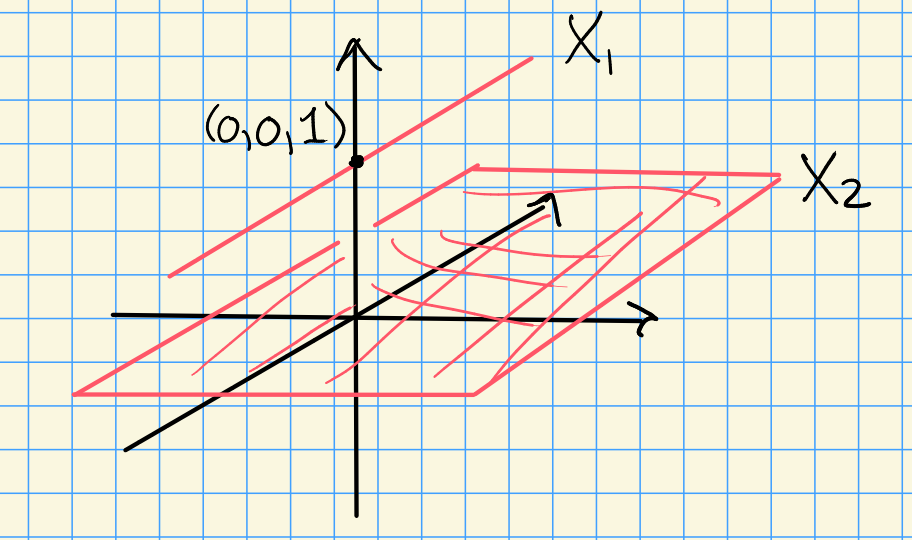
\includegraphics{figures/image_2020-09-01-10-43-00.png}
\caption{Image}
\end{figure}

\end{example}

\hypertarget{thursday-september-03}{%
\section{Thursday, September 03}\label{thursday-september-03}}

Recall that the Zariski topology is defined on an affine variety
\(X = V(J)\) with \(J \normal k[x_1, \cdots, x_n]\) by describing the
closed sets.

\begin{proposition}[?]

\(X\) is irreducible if its coordinate ring \(A(X)\) is a domain.

\end{proposition}

\begin{proposition}[?]

There is a 1-to-1 correspondence
\begin{align*}  
\correspond{\text{Irreducible subvarieties} \\ \text{of }X}
\iff
\correspond{\text{Prime ideals} \\ \text{in }A(X)}
.\end{align*}

\end{proposition}

\begin{proof}

Suppose \(Y\subset X\) is an affine subvariety. Then
\begin{align*}  
A(X) / I_X(Y) = A(Y)
.\end{align*}

By NSS, there is a bijection between subvarieties of \(X\) and radical
ideals of \(A(X)\) where \(Y\mapsto I_X(Y)\). A quotient is a domain iff
quotienting by a prime ideal, so \(A(Y)\) is a domain iff \(I_X(Y)\) is
prime.

\end{proof}

Recall that \(\mfp \normal R\) is prime when
\(fg\in \mfp \iff f\in \mfp\) or \(g\in \mfp\). Thus
\(\bar f \bar g = 0\) in \(R/\mfp\) implies \(\bar f = 0\) or
\(\bar g = 0\) in \(R/\mfp\), i.e.~\(R/\mfp\) is a domain.

Finally note that prime ideals are radical (easy proof).

\begin{example}

Consider \(\AA^2/\CC\) and some subvarieties \(C_i\):

\begin{figure}
\centering
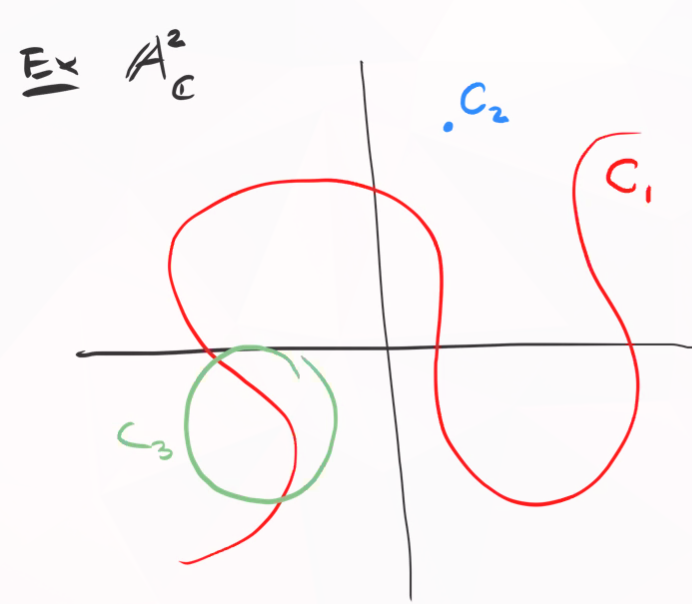
\includegraphics{figures/image_2020-09-03-09-47-09.png}
\caption{Subvarieties}
\end{figure}

Then irreducible subvarieties correspond to prime ideals in
\(\CC[x, y]\). Here \(C_1, C_3\) correspond to \(V(f), V(g)\) for
\(f,g\) irreducible polynomials, whereas \(C_2\) corresponds to a
maximal ideal, i.e.~\(V(x_1 - a_1, x_2 - a_2)\).

Note that \(I(C_1 \union C_2 \union C_3)\) is not a prime ideal, since
the variety is reducible as the union of 3 closed subsets.

\end{example}

\begin{example}

A finite set is irreducible iff it contains only one point.

\end{example}

\begin{example}

Any irreducible topological space is connected, since irreducible
requires a union but connectedness requires a \emph{disjoint} union.

\end{example}

\begin{example}

\(\AA^n/k\) is irreducible: by prop 2.8, its irreducible iff the
coordinate ring is a domain. However \(A(\AA^n) = k[x_1, \cdots, x_n]\),
which is a domain.

\end{example}

\begin{example}

\(V(x_1 x_2)\) is not irreducible, since it's equal to
\(V(x_1) \union V(x_2)\).

\end{example}

\begin{definition}[Noetherian Space]

A \emph{Noetherian} topological space \(X\) is a space with no infinite
strictly decreasing sequence of closed subsets.

\end{definition}

\begin{proposition}[?]

An affine variety \(X\) with the zariski topology is a noetherian space.

\end{proposition}

\begin{proof}

Let \(X_0 \supsetneq X_1 \supsetneq \cdots\) be a decreasing sequence of
closed subspaces. Then \(I(X_0) \subsetneq I(X_1) \subsetneq\). Note
that these containments are strict, otherwise we could use
\(V(I(X_1)) = X_1\) to get an equality in the original chain.

Recall that a ring \(R\) is Noetherian iff every ascending chain of
ideals terminates. Thus it suffices to show that \(A(X)\) is Noetherian.

We have \(A(X) = \kx{n} / I(X)\), and if this had an infinite chain
\(I_1 \subsetneq I_2 \subsetneq \cdots\) lifts to a chain in \(\kx{n}\),
which is Noetherian. A useful fact: \(R\) noetherian implies that
\(R[x]\) is noetherian, and fields are always noetherian.

\end{proof}

\begin{remark}

Any subspace \(A\subset X\) of a noetherian space is noetherian. To see
why, suppose we have a chain of closed sets in the subspace topology,
\begin{align*}  
A\intersect X_0 \supsetneq A\intersect X_1 \supsetneq \cdots
.\end{align*}

Then \(X_0 \supsetneq X_1 \supsetneq \cdots\) is a strictly decreasing
chain of closed sets in \(X\). Why strictly decreasing:
\(\intersect^n X_i = \intersect^{n+1} X_i \implies A\intersect^n X_i = A\intersect^{n+1} X_i\),
a contradiction.

\end{remark}

\begin{proposition}[Important]

Every noetherian space \(X\) is a finite union of irreducible closed
subsets, i.e.~\(X = \Union_{i=1}^k X_i\). If we further assume
\(X_i \not\subset X_j\) for all \(i, j\), then the \(X_i\) are unique up
to permutation.

\end{proposition}

\begin{remark}

The \(X_i\) are the \textbf{components} of \(X\). In the previous
example \(C_1 \union C_2 \union C_3\) has three components.

\end{remark}

\begin{proof}

If \(X\) is irreducible, then \(X=X\) and this holds.

Otherwise, write \(X = X_1 \union X_2\) with \(X_i\) proper closed
subsets. If \(X_1\) and \(X_1'\) are irreducible, we're done, so
otherwise suppose wlog \(X_1'\) is not irreducible.

Then we can express \(X = X_1 \union \qty{X_2 \union X_2'}\) with
\(X_2, X_2' \subset X_1'\) closed and proper.

Thus we can obtain a tree whose leaves are proper closed subsets:

\begin{figure}
\centering
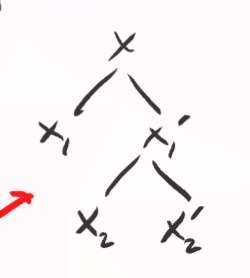
\includegraphics{figures/image_2020-09-03-10-15-53.png}
\caption{Image}
\end{figure}

This tree terminates because \(X\) is Noetherian: if it did not, this
would generate an infinite decreasing chain of subspaces.

We now want to show that the decomposition is unique if no two
components are contained in the other.

Suppose
\begin{align*}  
X= \Union_{i=1}^k X_i = \Union_{j=1}^\ell X_j'
.\end{align*}

Note that \(X_i \subset X\) implies that
\(X_i = \Union_{j=1}^\ell X_i \intersect X_j'\). But \(X_i\) is
irreducible and this would express \(X_i\) as a union of proper closed
subsets, so some \(X_i \intersect X_j'\) is \emph{not} a proper closed
subset.

Thus \(X_i = X_i \intersect X_j'\) for some \(j\), which forces
\(X_i \subset X_j'\). Applying the same argument to \(X_j'\) to obtain
\(X_j' \subset X_k\) for some \(k\).

Then \(X_i \subset X_j' \subset X_k\), but \(X_ i \not\subset X_j\) when
\(j\neq i\). Thus \(X_i = X_j' = X_k\), forcing the \(X_i\) to be unique
up to permutation.

\end{proof}

Recall from ring theory: for \(I\subset R\) and \(R\) noetherian, \(I\)
has a \emph{primary decomposition} \(I = \Intersect_{i=1}^k Q_i\) with
\(\sqrt{Q_i}\) prime. Assuming the \(Q_i\) are minimal in the sense that
\(\sqrt{Q_i} \not\subset \sqrt{Q_j}\) for any \(i, j\), this
decomposition is unique.

Applying this to \(I(X) \normal \kx{n} = R\) yields
\begin{align*}  
I(X) = \Intersect_{i=1}^k Q_i 
\implies
X  = V(I(X)) = \Union_{i=1}^k V(Q_i)
.\end{align*}

Letting \(P_i = \sqrt{Q_i}\), noting that the \(P_i\) are prime and thus
radical, we have \(V(Q_i) = V(P_i)\). Writing \(X = \Union V(P_i)\), we
have \(I(V(P_i)) = P_i\) and thus \(A(V(P_i)) = R/P_i\) is a domain,
meaning \(V(P_i)\) are irreducible affine varieties.

Conversely, if we express \(X = \Union X_i\), we have
\(I = I\qty{\Union X_i} = \Intersect I(X_i) = \Intersect P_i\) which are
irreducible since they are prime.

\begin{remark}

There is a correspondence
\begin{align*}  
\correspond{\text{Irreducible components} \\ \text{of } X} 
\iff
\correspond{\text{Minimal prime ideals} \\ \text{in } A(X)}
,\end{align*} where here \emph{minimal} is the condition that no pair of
ideals satisfies a subset containment.

\end{remark}

\begin{remark}

Let \(X\) be an irreducible topological space.

\begin{proposition}[1]

The intersection of nonempty two open sets is \emph{never} empty.

\end{proposition}

\begin{proof}

Let \(U, U'\) be open and \(X\setminus U, X\sm U'\) closed. Then
\(U\intersect U' = \emptyset \iff (X\sm U) \union (X\sm U') = X\), but
this is not possible since \(X\) is irreducible.

\end{proof}

\begin{quote}
Irreducible iff any two nonempty open sets intersect.
\end{quote}

\begin{proposition}[?]

Any nonempty open set is dense, i.e.~if \(U\subset X\) is open then its
closure \(\cl_X(U)\) is dense in \(X\).

\end{proposition}

\begin{proof}

Write \(X = \cl_X(U) \union (X\sm U)\). Since \(X\sm U \neq X\) and
\(X\) is irreducible, we have \(\cl_X(U) = X\).

\end{proof}

\end{remark}

\hypertarget{tuesday-september-08}{%
\section{Tuesday, September 08}\label{tuesday-september-08}}

Review: we discussed irreducible components. Recall that the
\emph{Zariski topology} on an affine variety \(X\) has affine
subvarieties as closed sets, and a \emph{noetherian space} has no
infinitely decreasing chains of closed subspaces.

We showed that any noetherian space has a decomposition into irreducible
components \(X = \union X_i\) with \(X_i\) closed, irreducible, and
unique such that no two are subsets of each other. Applying this to
affine varieties, a descending chain of subspaces
\(X_0 \supsetneq X_1 \cdots\) in \(X\) corresponds to an increasing
chain of ideals \(I(X_0) \subsetneq I(X_1) \cdots\) in \(A(X)\). Since
\(\kx{n}\) is a noetherian ring, this chain terminates, so affine
varieties are noetherian.

\hypertarget{dimension}{%
\subsection{Dimension}\label{dimension}}

\begin{definition}[Dimensions]

Let \(X\) be a topological space.

\begin{enumerate}
\def\labelenumi{\arabic{enumi}.}
\item
  The \emph{dimension} \(\dim X \in \NN\union\ts{\infty}\) is either
  \(\infty\) or the length \(n\) of the longest chain of
  \textbf{irreducible} closed subsets
  \(\emptyset \neq Y_0 \subsetneq \cdots \subsetneq Y_n \subset X\)
  where \(Y_n\) need not be equal to \(X\).
\item
  The \emph{codimension} of \(Y\) in \(X\), \(\codim_X(Y)\), for an
  irreducible subset \(Y\subseteq X\) is the length of the longest chain
  \(Y\subset Y_0 \subsetneq Y_1 \cdots \subset X\).
\end{enumerate}

\end{definition}

\begin{example}

Consider \(\AA^1/k\), what are the closed subsets? The finite sets, the
empty set, and the entire space.

What are the irreducible closed subsets? Every point is a closed subset,
so sets with more than one point are reducible. So the only irreducible
closed subsets are \(\ts{a}, \AA^1/k\), since an affine variety is
irreducible iff its coordinate ring is a domain and
\(A(\AA^1/k) = k[x]\). We can check
\begin{align*}  
\emptyset \subseteq Y_0 = \ts{a} \subseteq Y_1 = \AA^1/k
,\end{align*}

which is of length \(1\), so \(\dim(\AA^1/k) = 1\).

\begin{quote}
Note that we count the number of nontrivial strict subset containments
in this chain.
\end{quote}

\end{example}

\begin{example}

Consider \(V(x_1 x_2) \subset \AA^2/k\), the union of the \(x_i\) axes.
Then the closed subsets are \(V(x_1), V(x_2)\), along with finite sets
and their unions. What is the longest chain of irreducible closed
subsets?

Note that \(k[x_1, x_2] / \gens{x_1} \cong k[x_2]\) is a domain, so
\(V(x_i)\) are irreducible. So we can have a chain
\begin{align*}  
\emptyset \subsetneq \ts{a} \subsetneq V(x_1) \subset X
,\end{align*} where \(a\) is any point on the \(x_2\dash\)axis, so
\(\dim(X) = 1\).

The only closed sets containing \(V(x_1)\) are \(V(x_1)\union S\) for
\(S\) some finite set, which can not be irreducible.

\end{example}

\begin{remark}

You may be tempted to think that if \(X\) is noetherian then the
dimension is finite. However, finite dimension requires a bounded length
on descending/ascending chains, whereas noetherian only requires
``termination'', which may not happen in a bounded number of steps. So
this is \textbf{false}!

\end{remark}

\begin{example}

Take \(X = \NN\) and define a topology by setting closed subsets be the
sets \(\ts{0, \cdots, n}\) as \(n\) ranges over \(\NN\), along with
\(\NN\) itself. Is \(X\) noetherian? Check descending chains of closed
sets:

\begin{align*}  
\NN \supsetneq \ts{0, \cdots, N} \supsetneq \ts{0, \cdots, N-1} \cdots
,\end{align*}

which has length at most \(N\), so it terminates and \(X\) is
noetherian.

But note that all of these closed subsets \(X_N \da \ts{0, \cdots, N}\)
are irreducible. Why? If \(X_n = X_i \union X_j\) then one of \(i, j\)
is equal to \(N\), i.e \(X_i, X_j = X_N\).

So for every \(N\), there exists a chain of irreducible closed subsets
of length \(N\), implying that \(\dim(\NN) = \infty\).

\end{example}

\begin{remark}

Let \(X\) be an affine variety. There is a correspondence
\begin{align*}  
\correspond{\text{Chains of irreducible closed subsets} \\ Y_0 \subsetneq \cdots \subsetneq Y_n \text{ in } X}
\correspond{\text{Chains of prime ideals} \\ P_0\supsetneq \cdots \supsetneq P_n \text{ in } A(X)}
.\end{align*} Why? We have a correspondence between closed subsets and
radical ideals. If we specialize to irreducible, we saw that these
correspond to radical ideals \(I\subset A(X)\) such that
\(A(Y) \da A(X) / I\) is a domain, which precisely correspond to prime
ideal in \(A(X)\).

\end{remark}

We thus make the following definition:

\begin{definition}[Krull Dimension]

The \emph{krull dimension} of a ring \(R\) is the length \(n\) of the
longest chain of prime ideals
\begin{align*}  
P_0 \supsetneq P_1 \supsetneq \cdots \supsetneq P_n
.\end{align*}

\end{definition}

\begin{remark}

This uses the key fact from commutative algebra: a finitely generated
\(k\dash\)algebra \(M\) satisfies

\begin{enumerate}
\def\labelenumi{\arabic{enumi}.}
\tightlist
\item
  \(M\) has finite \(k\dash\)dimension
\item
  If \(M\) is a domain, every maximal chain has the same length.
\end{enumerate}

\end{remark}

\begin{remark}

From scheme theory: for any ring \(R\), there is an associated
topological space \(\spec R\) given by the set of prime ideals in \(R\),
where the closed sets are given by
\begin{align*}  
V(I) = \ts{\text{Prime ideals } \mfp \normal R \st I\subseteq \mfp }
.\end{align*}

If \(R\) is a noetherian ring, then \(\spec(R)\) is a noetherian space.

\end{remark}

\begin{example}

Using the fact above, let's compute \(\dim \AA^n/k\). We can take the
following chain of prime ideals in \(\kx{n}\):
\begin{align*}  
0 \subsetneq \gens{x_1} \subsetneq \gens{x_1, x_2} \cdots \subsetneq \gens{x_1, \cdots, x_n}
.\end{align*}

By applying \(V(\wait)\) we obtain
\begin{align*}  
\AA^n/k \supsetneq \AA^{n-1}/k \cdots \supsetneq \AA^0/k = \ts{0} \supsetneq \emptyset
,\end{align*} where we know each is irreducible and closed, and it's
easy to check that these are maximal:

If there were an ideal
\(\gens{x_1, x_2} \subset P \subset \gens{x_1, x_2, x_3}\), then take
\(P\intersect k[x_1, x_2, x_3] / \gens{x_1, x_2}\) which would yield a
polynomial ring in \(k[x_1]\). But we know the only irreducible sets in
\(\AA^1/k\) are a point and the entire space.

So this is a chain of maximal length, implying \(\dim \AA^n/k = n\).

\end{example}

\hypertarget{thursday-september-10}{%
\section{Thursday, September 10}\label{thursday-september-10}}

Recall that the dimension of a ring \(R\) is the length of the longest
chain of prime ideals. Similarly, for an affine variety \(X\), we
defined \(\dim X\) to be the length of the longest chain of irreducible
closed subsets.

These notions of dimension of the same when taking \(R = A(X)\),
i.e.~\(\dim \AA^n/k = n\).

\begin{proposition}[Dimensions]

Let \(k = \bar k\).

\begin{enumerate}
\def\labelenumi{\alph{enumi}.}
\tightlist
\item
  The dimension of \(k[x_1, \cdots, x_n]\) is \(n\).
\item
  All maximal chains of prime ideals have length \(n\).
\end{enumerate}

\end{proposition}

\hypertarget{proof-of-dimension-proposition}{%
\subsection{Proof of Dimension
Proposition}\label{proof-of-dimension-proposition}}

The case for \(n=0\) is trivial, just take \(P_0 = \gens{0}\). For
\(n=1\), easy to see since the only prime ideals in \(k[x]\) are
\(\gens{0}\) and \(\gens{x-a}\), since any polynomial factors into
linear factors.\\

Let \(P_0 \subsetneq \cdots \subsetneq P_m\) be a maximal chain of prime
ideals in \(\kx{n}\); we then want to show that \(m=n\). Assume
\(P_0 = \gens{0}\), since we can always extend our chain to make this
true (using maximality). Then \(P_1\) is a minimal prime and \(P_m\) is
a maximal ideal (and maximals are prime).

\begin{claim}

\(P_1\) is principle, i.e.~\(P_1 = \gens{f}\) for some irreducible
\(f\).

\end{claim}

\hypertarget{proof-that-p_1-is-principle}{%
\subsubsection{\texorpdfstring{Proof That \(P_1\) is
Principle}{Proof That P\_1 is Principle}}\label{proof-that-p_1-is-principle}}

\begin{claim}

\(\kx{n}\) is a unique factorization domain. This follows since \(k\) is
a UFD since it's a field, and \(R\) a UFD \(\implies R[x]\) is a UFD for
any \(R\).

\begin{quote}
See Gauss' lemma.
\end{quote}

\end{claim}

\begin{claim}

In a UFD, minimal primes are principal. Let \(r \in P\), and write
\(r = u \prod p_i^{n_i}\) with \(p_i\) irreducible and \(u\) a unit. So
some \(p_i\in P\), and \(p_i\) irreducible implies \(\gens{p_i}\) is
prime. Since \(0 \subsetneq \gens{p_i} \subset P\), but \(P\) was prime
and assumed minimal, so \(\gens{p_i} = P\).

\end{claim}

The idea is to now transfer the chain
\(P_0 \subsetneq \cdots \subsetneq P_m\) to a maximal chain in
\(k[x_1, \cdots, x_{n-1}]\). The first step is to make a linear change
of coordinates so that \(f\) is monic in the variable \(x_n\).

\begin{example}

Take \(f=x_1x_2 + x_3^2 x_4\) and map \(x_3 \mapsto x_3 + x_4\).

\end{example}

So write
\begin{align*}  
f(x_1, \cdots, x_n) = x_n^d + f_1(x_1, \cdots, x_{n-1}) x_n^{d-1} + \cdots + f_d(x_1, \cdots, x_{n-1})
.\end{align*}

We can then descend to \(\kx{n}\) to \(\kx{n}/\gens{f}\):

\begin{center}
\begin{tikzcd}
P_0 \ar[r] & P_1 \ar[r]\ar[d] & \cdots \ar[r]\ar[d] & P_m\ar[d] \\
 & P_1/P_1 \ar[r]\ar[d] & \cdots \ar[r]\ar[d] & P_m/P_1\ar[d] \\
 & P_1/P_1 \intersect \kx{n-1} \ar[r] & \cdots \ar[r] & (P_m / P_1) \intersect \kx{n-1}
\end{tikzcd}
\end{center}

The first set of downward arrows denote taking the quotient, and the
upward is taking inverse images, and this preserves strict inequalities.

\begin{definition}[Integral Extension]

An \emph{integral} ring extension \(R\injects R'\) of \(R\) is one such
that all \(r' \in R'\) satisfying a monic polynomial with coefficients
in \(R\), where \(R'\) is finitely generated.

\begin{quote}
In this case, also implies that \(R'\) is a finitely-generated \(R\)
module.
\end{quote}

\end{definition}

In this case, \(\kx{n-1} \injects \kx{n} /\gens{f}\) is an integral
extension. We want to show that the intersection step above also
preserves strictness of inclusions, since it preserves primality.

\begin{lemma}

Suppose \(P', Q' \subset R'\) are distinct prime ideals with
\(R\injects R'\) an integral extension. Then if
\(P'\intersect R = Q'\intersect R\), neither contains the other,
i.e.~\(P'\not\subset Q'\) and \(Q'\not\subset P'\).

\end{lemma}

\begin{proof}

Toward a contradiction, suppose \(P' \subset Q'\), we then want to show
that \(Q'\supset P'\). Let \(a\in Q'\sm P'\) (again toward a
contradiction), then
\begin{align*}  
R/\qty{P'\intersect R} \injects R'/P'
\end{align*} is integral.

Then \(\bar a \neq 0\) in \(R'/P'\), and there exists a monic polynomial
of minimal degree that \(\bar a\) satisfies,
\(p(x) = x^n + \sum_{i=2}^n \bar c_i x^{n-i}\). This implies
\(\bar c_n \in Q'/P'\) (which will contradict \(c_n \in P'\)), since if
\(\bar c_n = 0\) then factoring out \(x\) yields a lower degree
polynomial that \(\bar a\) satisfies.

But then \(\bar a_n \in Q'\intersect R\), so ???

\end{proof}

Question: Given \(R\injects R'\) is an integral extension, can we lift
chains of prime ideals?

Answer: Yes, by the ``Going Up'' Theorem: given \(P\subset R\) prime,
there exists \(P'\subset R'\) prime such that \(P'\intersect R = P\).
Furthermore, we can lift \(P_1 \subset P_2\) to \(P_1' \subset P_2'\),
as well as ``lifting sandwiches'':

\begin{figure}
\centering
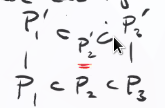
\includegraphics{figures/image_2020-09-10-10-18-40.png}
\caption{Image}
\end{figure}

In this process, the length of the chain decreased since \(\gens{0}\)
was deleted, but otherwise the chains are in bijective correspondence.
So the inductive hypothesis applies. \(\qed\)

\hypertarget{using-dimension-theory}{%
\subsection{Using Dimension Theory}\label{using-dimension-theory}}

Key fact used: the dimension doesn't change under integral extensions,
i.e.~if \(R\injects R'\) is integral then \(\dim R = \dim R'\).

\begin{claim}

Any affine variety has finite dimension.

\end{claim}

\begin{proof}

We have \(\dim X = \dim A(X)\), where \(A(X) \da \kx{n} I\) for some
\(I(X)=\sqrt{I(X)}\).

The noether normalization lemma (used in proof of nullstellensatz) shows
that a finitely generated \(k\dash\)algebra is an integral extension of
some polynomial ring \(k[y_1, \cdots, y_d]\). I.e., the following
extension is integral:
\begin{align*}  
k[y_1, \cdots, y_d] \injects k[x_1, \cdots, x_n]/I
.\end{align*}

We can conclude that \(\dim A(X) = d < \infty\).

\end{proof}

\begin{proposition}[?]

Let \(X, Y\) be irreducible affine varieties. Then

\begin{enumerate}
\def\labelenumi{\alph{enumi}.}
\tightlist
\item
  \(\dim X\cross Y = \dim X + \dim Y\).
\item
  \(Y\subset X \implies \dim X = \dim Y + \codim_X Y\).
\item
  If \(f\in A(X)\) is nonzero, then any component of \(V(f)\) has
  codimension 1.
\end{enumerate}

\end{proposition}

\begin{proof}

\begin{remark}

Why is \(X\cross Y\) again an affine variety? If \(X\subset \AA^n/k\),
\(Y\subset \AA^m/k\) with \(X = V(I), Y = V(J)\), then
\(X\cross Y \subset \AA^n/k \cross \AA^m/k = \AA^{n+m}/k\) can be given
by taking \(I+J \normal k[x_1, \cdots, x_n, y_1, \cdots, y_m]\) using
the natural inclusions of \(\kx{\ell}\).

Note that we can write
\begin{align*}  
k[x_1, \cdots, x_n, y_1, \cdots, y_m] = \kx{n} \tensor_k k[y_1, \cdots, y_n]
\end{align*} where we think of
\(x_i = x_i \tensor 1, y_j = 1 \tensor y_j\). We thus map \(I, J\) to
\(I\tensor 1 + 1\tensor J\) and obtain
\(V(I\tensor 1 + 1\tensor J) = X\cross Y\) and
\(A(X\cross Y) = A(X)\tensor_k A(Y)\).

In general, for \(k\dash\)algebras \(R,S\),
\begin{align*}  
R/I \tensor_k S/J \cong R\tensor_k S / \gens{I\tensor 1 + 1\tensor J}
.\end{align*}

\end{remark}

\begin{remark}

For \(R,S\) finitely generated \(k\dash\)algebras,
\(\dim R\tensor_k S = \dim R + \dim S\).

\end{remark}

Part (a) is proved by the above remarks.

For part (b), the statement is equivalent to \(P\subset A(X)\) with
\(I(Y) \subset P\) is a member of some maximal chain, along with the
statement that all maximal chains are the same length.

\end{proof}

\hypertarget{tuesday-september-15}{%
\section{Tuesday, September 15}\label{tuesday-september-15}}

\hypertarget{review}{%
\subsection{Review}\label{review}}

Let \(k=\bar k\), we're setting up correspondences
\begin{align*}  
\text{Ring Theory} 
\quad&\quad 
\text{Geometry/Topology of Affine Varieties}
\\
\text{Polynomial functions} 
\quad&\quad 
\text{Affine space} 
\\
k[x_1, \cdots, x_n]
\quad&\quad 
\AA^n/k \da \ts{\thevector{a_1, \cdots, a_n} \in k^n } 
\\
\text{Maximal ideals } \gens{x_1 - a_1, \cdots, x_n - a_n} 
\quad&\quad 
\text{Points } \thevector{a_1, \cdots, a_n} \in \AA^n/k
\\
\text{Radical ideals } I\normal k[x_1, \cdots, x_n]
\quad&\quad 
\text{Affine varieties } X\subset  \AA^n/k, \text{ vanishing locii of polynomials} 
\\
I &\mapsto V(I) \da \ts{a\st f(a) = 0 \forall f\in I} \\
I(X) \da \ts{f \st \restrictionof{f}{X} = 0} &\mapsfrom X 
\\
\text{Radical ideals containing $I(X)$, i.e. ideals in $A(X)$} 
\quad&\quad 
\text{closed subsets of $X$, i.e. affine subvarieties}
\\
A(X) \text{ is a domain}
\quad&\quad 
\text{$X$ irreducible}
\\
\text{$A(X)$ is not a direct sum}
\quad&\quad 
\text{$X$ connected} 
\\
\text{Prime ideals in }A(X)
\quad&\quad 
\text{Irreducible closed subsets of }X
\\
\text{Krull dimension $n$ (longest chain of prime ideals)}
\quad&\quad 
\dim X = n,\, \text{(longest chain of irreducible closed subsets)}
.\end{align*}

\begin{quote}
Recall that we defined the coordinate ring \(A(X) \da \kx{n} / I(X)\),
which contained no nilpotents.
\end{quote}

We had some results about dimension

\begin{enumerate}
\def\labelenumi{\arabic{enumi}.}
\tightlist
\item
  \(\dim X<\infty\) and \(\dim \AA^n = n\).
\item
  \(\dim Y + \codim_X Y = \dim X\) when \(Y\subset X\) is irreducible.
\item
  Only over \(\bar k = k\), \(\codim_X V(f) = 1\).
\end{enumerate}

\begin{example}

Take \(V(x^2+y^2) \subset \AA^2/\RR\)

\end{example}

\begin{definition}[?]

An affine variety \(Y\) of

\begin{itemize}
\tightlist
\item
  \(\dim Y = 1\) is a \textbf{curve},
\item
  \(\dim Y = 2\) is a \textbf{surface},
\item
  \(\codim_X Y = 1\) is a \textbf{hypersurface in \(X\)}
\end{itemize}

\end{definition}

Question: Is every hypersurface the vanishing locus of a \emph{single}
polynomials \(f\in A(X)\)?

Answer: This is true iff \(A(X)\) is a UFD.

\begin{definition}[Codimension in a Ring]

\(\codim_R \mfp\) is the length of the longest chain
\begin{align*}P_0 \subsetneq P_1 \subsetneq \cdots \subsetneq P_n = \mfp.\end{align*}

\end{definition}

Recall that \(f\) is irreducible if
\(f = f_1 f_2 \implies f_i \in R\units\) for one \(i\), and \(f\) is
prime iff \(\gens{f}\) is a prime ideal, or equivalently
\(f\divides ab \implies f\divides a\) or \(f\divides b\).

Note that prime implies irreducible, since \(f\) divides itself.

\begin{proposition}[?]

Let \(R\) be a Noetherian domain, then TFAE

\begin{enumerate}
\def\labelenumi{\alph{enumi}.}
\item
  All prime ideals of codimension 1 are principal.
\item
  \(R\) is a UFD.
\end{enumerate}

\end{proposition}

\begin{proof}

\(a\implies b\):

Let \(f\) be a nonzero non-unit, we'll show it admits a prime
factorization. If \(f\) is not irreducible, then \(f = f_1 f_1'\), both
non-units. If \(f_1'\) is not irreducible, we can repeat this, to get a
chain
\begin{align*}  
\gens{f} \subsetneq \gens{f_1'} \subsetneq \gens{f_2'} \subsetneq \cdots
,\end{align*} which must terminate.

This yields a factorization \(f = \prod f_i\) with \(f_i\) irreducible.
To show that \(R\) is a UFD, it thus suffices to show that the \(f_i\)
are prime. Choose a minimal prime ideal containing \(f\). We'll use
Krull's Principal Ideal Theorem: if you have a minimal prime ideal
\(\mfp\) containing \(f\), its codimension \(\codim_R \mfp\) is one. By
assumption, this implies that \(\mfp = \gens{g}\) is principal. But
\(g\divides f\) with \(f\) irreducible, so \(f,g\) differ by a unit,
forcing \(\mfp = \gens{f}\). So \(\gens{f}\) is a prime ideal.\\

\(b\implies a\):

Let \(\mfp\) be a prime ideal of codimension 1. If \(\mfp = \gens{0}\),
it is principal, so assume not. Then there exists some nonzero non-unit
\(f\in \mfp\), which by assumption has a prime factorization since \(R\)
is assumed a UFD. So \(f=\prod f_i\).

Since \(\mfp\) is a prime ideal and \(f\in\mfp\), some \(f_i\in \mfp\).
Then \(\gens{f_i} \subset \mfp\) and \(\mfp\) minimal implies
\(\gens{f_i} = \mfp\), so \(\mfp\) is principal.

\end{proof}

\begin{corollary}[?]

Every hypersurface \(Y\subset X\) is cut out by a single polynomial, so
\(Y=V(f)\), iff \(A(X)\) is a UFD.

\end{corollary}

\begin{example}

Apply this to \(R=A(X)\), we find that there is a bijection
\begin{align*}  
\codim 1 \text{ prime ideals}
\iff 
\codim 1 \text{ closed irreducible subsets }Y\subset X,\text{ i.e. hypersurfaces}
.\end{align*}

Taking \(A(X) = \CC[x,y,z]/\gens{x^2+y^2-z^2}\), whose real points form
a cone:

\begin{figure}
\centering
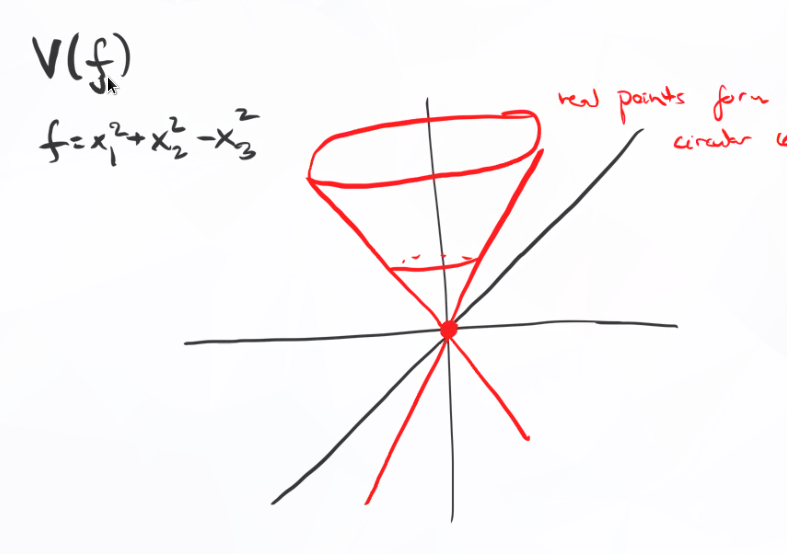
\includegraphics{figures/image_2020-09-15-10-26-24.png}
\caption{Image}
\end{figure}

Note that \(x^2 + y^2 = (x-iy)(x+iy) = z^2\) in this quotient, so this
is not a UFD.

Then taking a line through its surface is a codimension 1 subvariety not
cut out by a single polynomial. Such a line might be given by
\(V(x + iy, z)\), which is 2 polynomials, so why not codimension 2?

Note that \(V(z)\) is the union of the lines

\begin{itemize}
\tightlist
\item
  \(z = 0, x + iy= 0\),
\item
  \(z=0, x - iy = 0\).
\end{itemize}

Note that it suffices to show that this ring has an irreducible that is
not prime. Supposing \(z = f_1 f_2\), some \(f_i\) is a unit, then \(z\)
is not prime because \(z\divides xy\) but divides neither of \(x,y\).

\end{example}

\begin{example}

Note that \(\kx{n}\) is a UFD since \(k\) is a UFD. Applying the
corollary, every hypersurface in \(\AA^n\) is cut out by a single
irreducible polynomial.

\end{example}

\begin{definition}[?]

An affine variety \(X\) is of \textbf{pure dimension \(d\)} iff every
irreducible component \(X_i\) is of dimension \(d\).

\end{definition}

\begin{quote}
Note that \(X\) is a Noetherian space, so has a unique decomposition
\(X = \union X_i\).
\end{quote}

Given \(X\subset \AA^n/k\) of pure dimension \(n-1\), \(X = \union X_i\)
with \(X_i\) hypersurfaces with \(I(X_j) = \gens{f_j}\),
\(I(X) = \gens{f}\) where \(f = \prod f_i\).

\begin{definition}[?]

Given such an \(X\), define the \textbf{degree of a hypersurface} as the
degree of \(f\) where \(I(X) = \gens{f}\).

\end{definition}

\hypertarget{thursday-september-17}{%
\section{Thursday, September 17}\label{thursday-september-17}}

\hypertarget{regular-functions}{%
\subsection{Regular Functions}\label{regular-functions}}

\begin{quote}
See chapter 3 in the notes.
\end{quote}

Some examples:

\begin{itemize}
\tightlist
\item
  \(X\) a manifold or an open set in \(\RR^n\) has a ring of
  \(C^\infty\) functions.
\item
  \(X \subset \CC\) has a ring of holomorphic functions.
\item
  \(X\subset \RR\) has a ring of real analytic functions
\end{itemize}

These all share a common feature: it suffices to check if a function is
a member on an arbitrary open set about a point, i.e.~they are
\emph{local}.

\begin{definition}[?]

Let \(X\) be an affine variety and \(U\subseteq X\) open. A
\textbf{regular function} on \(U\) is a function \(\phi: U\to k\) such
that \(\phi\) is ``locally a fraction'', i.e.~a ratio of polynomial
functions.

More formally, for all \(p\in U\) there exists a \(U_p\) with
\(p\in U_p \subseteq U\) such that \(\phi(x) = g(x)/ f(x)\) for all
\(x\in U_p\) with \(f, g\in A(X)\).

\end{definition}

\begin{example}

For \(X\) an affine variety and \(f\in A(X)\), consider the open set
\(U\da V(f)^c\). Then \({1\over f}\) is a regular function on \(U\), so
for \(p\in U\) we can take \(U_p\) to be all of \(U\).

\end{example}

\begin{example}

For \(X = \AA^1\), take \(f=x-1\). Then \({x\over x-1}\) is a regular
function on \(\AA^1 \sm\ts{1}\).

\end{example}

\begin{example}

Let \(X + V(x_1 x_4 - x_2 x_3)\) and
\begin{align*}  
U \da X\sm V(x_2, x_4) = \ts{\thevector{x_1, x_2, x_3, x_4} \st x_1 x_4 = x_2 x_3, x_2\neq 0 \text{ or } x_4\neq 0 }
.\end{align*}

Define
\begin{align*}  
\phi: U &\to K \\
\thevector{x_1, x_2, x_3, x_4} &\mapsto
\begin{cases}
{x_1\over x_2} & \text{if } x_2 \neq 0 \\
{x_3\over x_4} & \text{if } x_4 \neq 0
\end{cases}
.\end{align*}

This is well-defined on \(\ts{x_2\neq 0} \intersect \ts{x_4 \neq 0}\),
since \({x_1\over x_2} = {x_3 \over x_4}\). Note that this doesn't
define an element of \(k\) at \(\thevector{0,0,0,1}\in U\). So this is
not globally a fraction.

\end{example}

Notation: we'll let \(\OO_X(U)\) is the ring of regular function on
\(U\).

\begin{proposition}[?]

Let \(U\subset X\) be an affine variety and \(\phi \in \OO_X(U)\). Then
\(V(\phi) \da \ts{x\in U \st \phi(x) = 0}\) is closed in the subspace
topology on \(U\).

\end{proposition}

\begin{proof}

For all \(a\in U\) there exists \(U_a\subset U\) such that
\(\phi = g_a/f_a\) on \(U_a\) with \(f_a, g_a \in A(X)\) with
\(f_a \neq 0\) on \(U_a\).

Then
\begin{align*}  
\ts{x\in U_a \st \phi(x) \neq 0} = U_a \sm V(g_a)\intersect U_a
\end{align*} is an open subset of \(U_a\), so taking the union over
\(a\) again yields an open set. But this is precisely \(V(\phi)^c\).

\end{proof}

\begin{proposition}

Let \(U\subset V\) be open in \(X\) an \emph{irreducible} affine
variety. If \(\phi_1, \phi_2 \in \OO_X(V)\) agree on \(U\), then they
are equal.

\end{proposition}

\begin{proof}

\(V(\phi_1 - \phi_2)\) contains \(U\) and is closed in \(V\). It
contains \(\bar U\intersect V\), by an earlier lemma, \(X\) irreducible
implies that \(\bar U = X\) and so \(V(\phi_1 - \phi_2) =V\).

\end{proof}

Compare and contrast: Let \(U\subset V \subset \RR^n\) be open. If
\(\phi_1, \phi_2 \in C^\infty(V)\) such that \(\phi_1, \phi_2\) are
equal when restricted \(U\subset V\). Does this imply
\(\phi_1 = \phi_2\)?

For \(\RR^n\), no, there exist smooth bump functions. You can make a
bump function on \(V\setminus U\) and extend by zero to \(U\). For
\(\CC\) and holomorphic functions, the answer is yes, by the uniqueness
of analytic continuation.

\begin{definition}[(Important) Distinguished Opens]

A \textbf{distinguished open set} in an affine variety is one of the
form
\begin{align*}  
D(f) \da X\sm V(f) = \ts{x\in X \st f(x) = 0}
.\end{align*}

\end{definition}

\begin{proposition}

The distinguished open sets form a base of the zariski topology.

\end{proposition}

\begin{proof}

Given \(f, g\in A(X)\), we can check:

\begin{enumerate}
\def\labelenumi{\arabic{enumi}.}
\tightlist
\item
  Closed under finite intersections: \(D(f) \intersect D(g) = D(fg)\).
\item

  \begin{align*}U = X\sm V(f_1, \cdots, f_k) = V\sm \bigcap V(f_i) = \bigcup D(f_i),\end{align*}
  and any open set is a \emph{finite} union of distinguished opens by
  the Hilbert basis theorem.
\end{enumerate}

\end{proof}

\begin{proposition}[?]

The regular functions on \(D(f)\) are given by
\begin{align*}  
\OO_X(D(f)) = \ts{{ g \over f^n} \st g\in A(X), n\in \NN} = A(X)_{\gens{f}}
,\end{align*} the localization of \(A(X)\) at \(\gens{f}\).

\end{proposition}

Note that if \(f=1\), then \(\OO_X(X) = A(X)\).

\begin{proposition}[?]

Note that \({g\over f^n} \in \OO_X(D(f))\) since \(f^n\neq 0\) on
\(D(f)\). Let \(\phi: D(f) \to k\) be a regular function. By definition,
for all \(a\in D(f)\) there exists a local representation as a fraction
\(\phi = g_a/f_a\) on \(U_a\ni a\). Note that \(U_a\) can be covered by
distinguished opens, one of which contains \(a\). Shrink \(U_a\) if
necessary to assume it is a distinguished open set \(U_a = D(h_a)\).\\

Now replace
\begin{align*}  
\phi = {g_a \over f_a} = {g_a h_a \over f_a h_a}
,\end{align*} which makes sense because \(h_a\neq 0\) on \(U_a\). We can
assume wlog that \(h_a = f_a\). Why? We have \(\phi = {g_a \over f_a}\)
on \(D(f_a)\). Since \(f_a\) doesn't vanish on \(U_a\), we have
\(V(f_a h_a) = V(h_a)\) since \(V(f_a) \subset D(h_a)^c = V(h_a)\).

Consider \(U_a = D(f_a)\) and \(U_b = D(f_b)\), on which
\(\phi = {g_a\over f_a}\) and \(\phi = {g_b \over f_b}\) respectively.
On \(U_a\intersect U_b = D(f_a f_b)\), these are equal,
i.e.~\(f_b g_a = f_a g_b\) in the coordinate ring \(A(X)\).\\

Then \(D(f) = \bigcup_a D(f_a)\), so take the component
\(V(f) = \intersect V(f_a)\) by the Nullstellensatz
\(f\in I(V(f_a)) = I(V(g_a, a\in D_f)) = \sqrt{f_a \st a\in D_f}\).

Then there exists an expression \(f^n = \sum k_a f_a\) as a finite sum,
so set \(g - \sum g_a k_a\).

\begin{claim}

\(\phi = g/f^n\) on \(D(f)\).\\

This follows because on \(D(f_b)\), we have \(\phi = {g_b \over f_b}\),
and so \(gf_b = \sum k_a g_a f_b\).

\end{claim}

\begin{quote}
Finish next class
\end{quote}

\end{proposition}

\hypertarget{tuesday-september-22}{%
\section{Tuesday, September 22}\label{tuesday-september-22}}

\hypertarget{review-regular-functions}{%
\subsection{Review: Regular Functions}\label{review-regular-functions}}

Given an affine variety \(X\) and \(U\subseteq X\) open, a \emph{regular
function} \(\phi: U\to k\) is one locally (wrt the zariski topology) a
fraction. We write the set of regular functions as \(\OO_X\).

\begin{example}

\(X = V(x_1 x_4 - x_2 x_3)\) on \(U = V(x_2, x_4)^c\), the following
function is regular:
\begin{align*}  
\phi: U &\to k \\
x &\mapsto 
\begin{cases}
{x_1\over x_2} & x_2 \neq 0 \\ \\
{x_3 \over x_4} & x_4 \neq 0
\end{cases}
.\end{align*} Note that this is not globally a fraction.

\end{example}

\begin{definition}[Distinguished Open Sets]

A \emph{distinguished open set} \(D(f) \subseteq X\) for some
\(f\in A(X)\) is \(V(f)^c \da \ts{x\in X \st f(x) \neq 0}\).

\end{definition}

These are useful because the \(D(f)\) form a base for the zariski
topology.

\begin{proposition}[?]

For \(X\) an affine variety, \(f\in A(X)\), we have
\begin{align*} 
\OO_X(D(f)) = \ts{ {g\over f^n} \st g\in A(X), n\in \NN}
.\end{align*}

\end{proposition}

\begin{proof}

The first reduction we made was that \(\phi \in \OO_X(D(f))\) is
expressible as \(g_a\over f_a\) on distinguished opens \(D(f_a)\)
covering \(D(f)\). We also noted that
\begin{align*}
{g_a \over f_a} = {g_b \over f_b} \text{ on } D(f_a) \intersect D(f_b) \implies f_b g_a = f_a g_b \text{ in } A(X)
.\end{align*}\\

The second step was writing \(D(f) = \union D(f_a)\), and so
\(V(f) = \intersect_a V(f_a)\) implies that
\(f\in I(V(\ts{f_a \st a\in U}))\). By the Nullstellensatz,
\(f\in \sqrt{\gens{f_a \st a\in U}}\), so \(f^N = \sum k_a f_a\) for
some \(N\). So construct \(g = \sum k_a g_a\), then compute
\begin{align*}  
gf_b = \sum_a k_a g_a f_b = \sum_a k_a g_b f_a = g_b \sum k_a f_a = g_b f^N
.\end{align*} Thus \(g/f^N = g_b / f_b\) for all \(b\), and we can thus
conclude
\begin{align*}  
\phi \da \ts{{g_b \over f_b} \text{ on } D(f_b)} = g/f^N
.\end{align*}

\end{proof}

\begin{corollary}[?]

For \(X\) an affine variety, \(\OO_X(X) = A(X)\).

\end{corollary}

\begin{warnings}

For \(k\) not algebraically closed, the proposition and corollary are
both false. Take \(X = \AA^1/\RR\), then \({1\over x^2+1} \in \RR(x)\),
but \(\OO_X(X) \neq A(X) = \RR[x]\).

\end{warnings}

\begin{definition}[Localization]

Let \(R\) be a ring and \(S\) a set closed under multiplication, then
the localization at \(S\) is defined by
\begin{align*}  
R_S \da \ts{r/s \st r\in R, s\in S} / \sim
.\end{align*} where
\(r_1/s_1 \sim r_2/s_2 \iff s_3(s_2 r_1 - s_1 r_2) = 0\) for some
\(s_3 \in S\).

\end{definition}

\begin{example}

Let \(f\in R\) and take \(S = \ts{f^n \st n\geq 1}\), then
\(R_f \da R_S\).

\end{example}

\begin{corollary}[?]

\(\OO_X(D(f)) = A(X)_f\) is the localization of the coordinate ring.

\end{corollary}

These requires some proof, since the LHS literally consists of functions
on the topological space \(D(f)\) while the RHS consists of formal
symbols.

\begin{proof}

Consider the map
\begin{align*}  
A(X)_f &\to \OO_X(D(f)) \\
``g/f^n" &\mapsto g/f^n: D(f) \to k
.\end{align*}

By definition, there exists a \(k\geq 0\) such that
\begin{align*}  
f^k(f^m g - f^n g') = 0 
\implies
f^k(f^m g - f^n g') = 0 \text{ as a function on } D(f)
.\end{align*} Since \(f^k \neq 0\) on \(D(f)\), we have
\(f^m g = f^n g'\) as a function on \(D(f)\), so \(g/f^n = g'/g^m\) as
functions on \(D(f)\).\\

\textbf{Surjectivity}: By the proposition, we have surjectivity,
i.e.~any element of \(|OO_x(D(f))\) can be represented by some
\(g/f^n\).\\

\textbf{Injectivity}: Suppose \(g/f^n\) defines the zero function on
\(D(f)\), then \(g = 0\) on \(D(f)\) implies that \(fg=0\) on \(X\)
(i.e.~\(fg= 0 \in A(X)\)), and we can write
\(f(g\cdot 1 - f^n\cdot 0) = 0\). Then \(g/f^n\sim 0/1 \in A(X)_f\),
which forces \(g/f^n = 0\in A(X)_f\).

\end{proof}

\hypertarget{sheaves}{%
\subsection{Sheaves}\label{sheaves}}

Idea: spaces on functions on topological spaces.

\begin{definition}[Presheaf]

A \emph{presheaf} (of rings) \(\mathcal{F}\) on a topological space is

\begin{enumerate}
\def\labelenumi{\arabic{enumi}.}
\item
  For every open set \(U\subset X\) a ring \(\mathcal{F}(U)\).
\item
  For any inclusion \(U\subset V\) a restriction map
  \(\res_{VU}: \mathcal{F}(V) \to \mathcal{F}(U)\) satisfying
\end{enumerate}

\begin{enumerate}
\def\labelenumi{\alph{enumi}.}
\tightlist
\item
  \(F(\emptyset) = 0\).
\item
  \(\res_{UU} = \id_{\mathcal{F}(U)}\).
\item
  \(\res_{VW} \circ \res_{UV} = \res_{UW}\).
\end{enumerate}

\end{definition}

\begin{example}

The smooth functions on \(\RR\) with the standard topology,
\(\mathcal{F} = C^\infty\) where \(C^\infty(U)\) is the set of smooth
functions \(U\to \RR\). It suffices to check the restriction condition,
but the restriction of a smooth function is smooth: if \(f\) is smooth
on \(U\), it is smooth at every point in \(U\), i.e.~all derivatives
exist at all points of \(U\). So if \(V\subset U\), all derivatives of
\(f\) will exist at points \(x \in V\), so \(f\) will be smooth on
\(V\).

Note that this also works with continuous functions.

\end{example}

\begin{definition}[Sheaf]

A \emph{sheaf} is a presheaf satisfying an additional gluing property:
given \(\phi_i \in \mathcal{F}(U_i)\) such that
\(\restrictionof{\phi_i}{U_i\intersect U_j} = \restrictionof{\phi_j}{U_i \intersect U_j}\),
then there exists a unique \(\phi\in \mathcal{F}(\union_i U_i)\) such
that \(\restrictionof{\phi}{U_i} = \phi_i\).

\end{definition}

\hypertarget{thursday-september-24}{%
\section{Thursday, September 24}\label{thursday-september-24}}

Recall that we defined the \emph{regular functions} \(\OO_X(U)\) on an
open set \(U\subset X\) an affine variety as the set of functions
\(\phi: U\to k\) such that \(\phi\) is locally a fraction, i.e.~for all
\(p\in U\) there exists a neighborhood of \(p\), say \(U_p \subset U\),
such that \(\phi\) restricted to \(U_p\) is given by \(g_p \over f_p\)
for some \(f_p, g_p \in A(X)\).

We proved that on a distinguished open set \(D(f) = V(f)^c\), we have
\(\OO_X(D(f)) = A(X)_f\). An important example was that
\(\OO_X(X) = A(X)\).

Question: If \(X\) is a variety over \(\CC\), does \(A(X) = \Hol(X)\)?
The answer is no, since taking \(\AA^1/\CC \cong \CC = X\) we obtain
\(A(X) = \CC[x]\) but for example \(e^z \in \Hol(X)\).

On the other hand, if you require that \(f\in \Hol(X)\) is meromorphic
at \(\infty\), i.e.~\(f({1\over z})\) is meromorphic at zero, then you
do get \(\CC[z]\). This is an example of GAGA!

\begin{quote}
Review: what is a category?
\end{quote}

\begin{quote}
Review: what is a presheaf?
\end{quote}

\hypertarget{tuesday-september-29}{%
\section{Tuesday, September 29}\label{tuesday-september-29}}

Recall the definition of a presheaf: a sheaf of rings on a space is a
contravariant functor from its category of open sets to ring, such that

\begin{enumerate}
\def\labelenumi{\arabic{enumi}.}
\tightlist
\item
  \(F(\emptyset) = 0\)
\item
  The restriction from \(U\) to itself is the identity,
\item
  Restrictions compose.
\end{enumerate}

Examples:

\begin{itemize}
\tightlist
\item
  Smooth functions on \(\RR^n\)
\item
  Holomorphic functions on \(\CC\)
\end{itemize}

Recall the definition of sheaf: a presheaf satisfying \emph{unique}
gluing: given \(f_i \in \mathcal{F}(U_i)\), such that
\(\restrictionof{f_i}{U_i \intersect U_j} = \restrictionof{f_j}{U_i\intersect U_j}\)
implies that there exists a unique \(f\in \mathcal{F}(\union U_i)\) such
that \(\restrictionof{f}{U_i} = f_i\).

Question: Are the constant functions on \(\RR\) a presheaf and/or a
sheaf?

Answer: This is a presheaf but not a sheaf. Set
\(\mathcal{F}(U) = \ts{f: U\to \RR \st f(x) = c} \cong \RR\) with
\(\mathcal{F}(\emptyset) = 0\). Can check that restrictions of constant
functions are constant, the composition of restrictions is the overall
restriction, and restriction from \(U\) to itself gives the function
back.

Given constant functions \(f_i \in \mathcal{F}(U_i)\), does there exist
a unique constant function \(\mathcal{F}(\union U_i)\) restricting to
them? No: take \(f_1 = 1\) on \((0, 1)\) and \(f_2 = 2\) on \((2, 3)\).
Can check that they both restrict to the zero function on the
intersection, since these sets are disjoint.

How can we make this into a sheaf? One way: weaken the topology. Another
way: define another presheaf \(\mathcal{G}\) on \(\RR\) given by
\emph{locally} constant function,
i.e.~\(\ts{f: U\to \RR \st \forall p\in U, \exists U_p\ni p,\, \ro{f}{U_p} \text{ is constant}}\).
Reminiscent of definition of regular functions in terms of local
properties.

\begin{example}

Let \(X = \ts{p, q}\) be a two-point space with the discrete topology,
i.e.~every subset is open. Then define a sheaf by
\begin{align*}  
\emptyset &\mapsto 0 \\
\ts{p} &\mapsto R \\
\ts{q} &\mapsto S \\
\implies \ts{p, q} &\mapsto R\cross S
,\end{align*} where the sheaf condition forces the assignment of the
whole space to be the product. Note that the first 3 assignments are
automatically compatible, which means that we need a unique
\(f\in \mathcal{F}(X)\) restricting to \(R\) and \(S\). In other words,
\(\mathcal{F}(X)\) needs to be unique and have maps to \(R, S\), but
this is exactly the universal property of the product.

\end{example}

\begin{example}

Consider the presheaf on \(X\) given by
\(\mathcal{F}(X) = R\cross S \cross T\). Taking \(T = \ZZ/2\ZZ\), we can
force uniqueness to fail: by projecting to \(R, S\), there are two
elements in the fiber, namely \((r,s,0)\mapsto r,s\) and
\((r,s,1)\mapsto r,s\).

\end{example}

\begin{example}

Let \(X = \ts{a, b, c}\) and
\(\tau = \ts{\emptyset, \ts{a}, \ts{a, b}, \ts{a, c}}\). Can check that
it's closed under finite intersections and arbitrary unions, so this
forms a topology. Now make the assignments
\begin{align*}  
\ts{a}& \mapsto A \\
\ts{b}& \mapsto B \\
\ts{a, b}& \mapsto C \\
X &\mapsto ?
.\end{align*}

We have a situation like this:

\begin{center}
\begin{tikzcd}
& \mathcal{F}(X)\ar[ld]\ar[rd] & \\
B\ar[rd] & & C\ar[ld] \\
& A\ar[d] & \\
& \emptyset &
\end{tikzcd}
\end{center}

Unique gluing says that given \(r\in B, s\in C\) such that
\(\phi_B(r) = \phi_C(s)\), there should exist a unique
\(t\in \mathcal{F}(X)\) such that \(\ro{t}{\ts{a, b}} = r\) and
\(\ro{t}{\ts{a, c}} = s\). This recovers exactly the fiber product.
\begin{align*}  
B \cross_A C \da \ts{(r, s) \in B\cross C \st \phi_B(r) = \phi_C(s) \in A}
.\end{align*}

\end{example}

\begin{example}

Let \(X\) be an affine variety with the Zariski topology and let
\(\mathcal{F} \da \OO_X\) be the sheaf of regular functions:
\begin{align*}  
\OO_X(U) \da \ts{f: U\to k \st \forall p\in U,\, \exists U_p \ni p,\,\, \ro{f}{U_p} ={g_p \over h_p} }
.\end{align*}

Is this a presheaf? We can check that there are restriction maps:
\begin{align*}  
\OO_X(U) &\to \OO_X(V) \\
\ts{f: U\to K} &\mapsto \ts{\ro{f}{V}(x) \da f(x) \text{ for } x \in V }
.\end{align*} This makes sense because if \(V\subset U\), any \(x\in V\)
is in the domain of \(f\). Given that \(f\) is locally a fraction, say
\(\rho = g_p / h_p\) on \(U_p \ni p\), is \(\ro{\phi}{V}\) locally a
fraction? Yes: for all \(p\in V\subset U\), \(\phi = g_p / f_p\) on
\(U_p\) and this remains true on \(U_p \intersect V\).

To check that \(\OO_X\) is a sheaf, given a set of regular functions
\(\ts{\phi_i: U_i \to k}\) agreeing on intersections, define
\begin{align*}  
\phi: \union U_i &\to k\\
\phi(x) &\da \phi_i(x) \text{ if }x\in U_i
.\end{align*}

This is well-defined, since if \(x\in U_i \intersect U_j\),
\(\phi_i(x) = \phi_j(x)\) since both restrict to the same function on
\(U_i \intersect U_j\) by assumption.

Why is \(\phi\) locally a fraction? We need to check that for all
\(p\in U \da \union U_i\) there exists a \(U_p \ni p\) with
\(\ro{\phi}{U_p} = g_p/h_p\). But any \(p\in \union U_i\) implies
\(p\in U_i\) for some \(i\). Then there exists an open set
\(U_{i, p} \ni p\) in \(U_i\) such that
\(\ro{\phi}{U_{i, p}} = g_p / h_p\) by definition of a regular function.
So take \(U_p = U_{i, p}\) and use the fact that
\(\ro{\phi}{U_i} = \phi_i\) along with compatibility of restriction.

\end{example}

\begin{remark}

General observation: any presheaf of functions is a sheaf when the
functions are defined by a local property, i..e any property that can be
checked at \(p\) by considering an open set \(U_p \ni p\).

As in the examples of smooth or holomorphic functions, these were local
properties. E.g. checking that a function is smooth involves checking on
an open set around each point. On the other hand, being a constant
function is not a local property.

\end{remark}

\begin{definition}[Restriction of a (Pre)sheaf]

Given a sheaf \(\mathcal{F}\) on \(X\) and an open set \(U\subset X\),
we can define a sheaf \(\ro{\mathcal{F}}{U}\) on \(U\) (with the
subspace topology) by defining
\(\ro{\mathcal{F}}{U}(V) \da \mathcal{F}(V)\) for \(U\subseteq V\).

\end{definition}

\begin{definition}[Stalks]

Let \(\mathcal{F}\) be a sheaf on \(X\) and \(p\in X\) a point. The
\emph{stalk} of \(\mathcal{F}\) at \(p\), denoted \(\mathcal{F}_p\) for
\(p\in U\), is defined by
\begin{align*}  
\mathcal{F}_p \da \ts{(U, \phi) \st \phi \in \mathcal{F}(U) } / \sim
\end{align*} where \((U, \phi) \sim (V, \phi')\) iff there exists a
\(W\subset U\intersect V\) and \(p\in W\) such that
\(\ro{\phi}{W} = \ro{\phi}{W}'\).

\end{definition}

\begin{example}

What is the stalk of \(\Hol(\CC)\) at \(p=0\)?

Examples of equivalent elements in this stalk:

\begin{figure}
\centering
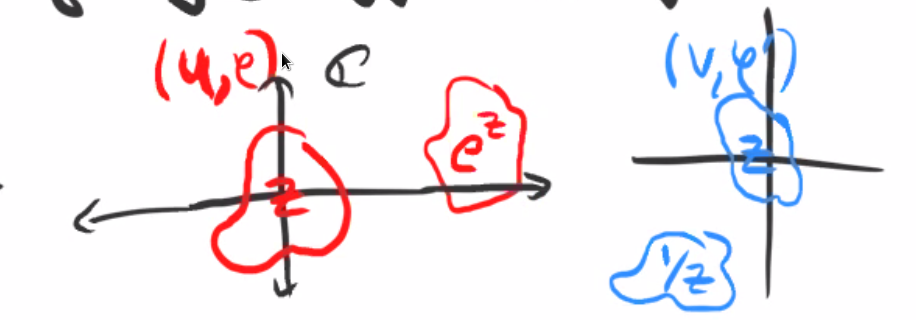
\includegraphics{figures/image_2020-09-29-10-38-22.png}
\caption{O}
\end{figure}

In this case
\begin{align*}  
\Hol(\CC)_0 = \ts{\phi = \sum_{i>0}c_i z^i \st \phi \text{ has a positive radius of convergence}}
.\end{align*}

\end{example}

\begin{definition}[Sections]

An element \(f\in \mathcal{F}(U)\) is called a \emph{section} over
\(U\), and elements of the stalk \(f\in \mathcal{F}_p\) are called
\emph{germs} at \(p\).

\end{definition}

\hypertarget{thursday-october-01}{%
\section{Thursday, October 01}\label{thursday-october-01}}

\hypertarget{stalks-and-localizations}{%
\subsection{Stalks and Localizations}\label{stalks-and-localizations}}

Recall that a sheaf of rings on a topological space \(X\) is a ring
\(\mathcal{F}(U)\) for all open sets \(U\subset X\) satisfying four
properties:

\begin{enumerate}
\def\labelenumi{\arabic{enumi}.}
\item
  The empty set is mapped to zeor.
\item
  The morphism \(\mathcal{F}(U)\to \mathcal{F}(U)\) is the identity.
\item
  Given \(W\subset V\subset U\) we have
\item
  Gluing: given sections \(s_i \in\mathcal{F}(U_i)\) which agree on
  overlaps (restrict to the same function on \(U_i\intersect U_j\)),
  there is a unique \(s\in \mathcal{F}(\union U_i)\).
\end{enumerate}

\begin{example}

If \(X\) is an affine variety with the zariski topology,
\(\mathcal{O}_X\) is a sheaf of regular functions, where we recall
\(\mathcal{O}_X(U)\) are the functions \(\phi: U\to k\) that are locally
a fraction.

\end{example}

Recall that the \emph{stalk} of a sheaf \(\mathcal{F}\) at a point
\(p\in X\), is defined as
\begin{align*}  
\mathcal{F}_p \da \ts{(U, \phi) \st p\in U \text{ open },\, \phi \in \mathcal{F}(U)}/\sim
.\end{align*} where \((U, \phi) \sim (U', \phi')\) if there exists a
\(p\in W \subset U\intersect U'\) such \(\phi, \phi'\) restricted to
\(W\) are equal.

Recall that a \emph{local ring} is a ring with a unique maximal ideal
\(\mfm\). Given a prime ideal \(\mfp \in R\), so
\(ab\in \mfp \implies a,b\in \mfp\), the complement \(R\setminus P\) is
closed under multiplication. So we can localize to obtain
\(R_\mfp = \ts{a/s \st s\in R\setminus P, a\in R}/\sim\) where
\(a'/s' \sim a/s\) iff there exists a \(t\in R\sm P\) such that
\(t(a's - as') = 0\).

\begin{warnings}

Note that \(R_f\) is localizing at the powers of \(f\), whereas
\(R_\mfp\) is localizing at the \emph{complement} of \(\mfp\).

\end{warnings}

Since maximal ideals are prime, we can localize any ring \(R\) at a
maximal ideal \(R_\mfm\), and this will be a local ring. Why? The ideals
in \(R_\mfm\) biject with ideals in \(R\) contained in \(\mfm\). Thus
all ideals in \(R_\mfm\) are contained in the maximal ideal generated by
\(\mfm\), i.e.~\(\mfm R_\mfm\).

\begin{lemma}[?]

Let \(X\) be an affine variety. The stalk of the sheaf of regular
functions \(\OO_{X, p} \da (\OO_X)_p\) is isomorphic to the localization
\(A(X)_{\mfm_p}\) where \(\mfm_p \da I(\ts{p})\).

\end{lemma}

\begin{proof}

We can write
\begin{align*}  
A(X)_{\mfm_p} \da \ts{{g\over f} \st g\in A(X),\, f\in A(X)\sm \mfm_p} / \sim \\
\text{ where } g_1/f_1 \sim g_2/f_2 \iff \exists h(p) \neq 0 \text{ where }0 = h(f_2 g_1 - f_1 g_2)
.\end{align*} where the \(f\) are regular functions on \(X\) such that
\(f(p) = 0\).

We can also write
\begin{align*}  
\OO_{X, p} \da \ts{(U, \phi) \st p\in U,\, \phi \in \OO_X(U) } /\sim 
\\ \text{ where } (U, \phi) \sim (U', \phi') 
\iff \exists p\in W \subset U\intersect U' \text{ s.t. } \ro{\phi}{W} = \ro{\phi'}{W}
.\end{align*}

So we can define a map
\begin{align*}  
\Phi: A(X)_{\mfm_p} &\to \OO_{X, p} \\
{g\over f} &\mapsto \qty{D_f, {g\over f}}
.\end{align*}

\textbf{Step 1:} There are equivalence relations on both sides, so we
need to check that things are well-defined.

We have
\begin{align*}  
g/f \sim g'/f' &\iff \exists g \text{ such that } h(p) \neq 0,\, h(gf' - g'f)=0 \in A(X) \\
&\iff \text{the functions } {g\over f}, {g' \over f'} \text{ agree on } W\da D(f) \intersect D(f') \intersect D(h) \\
&\implies (D_f, g/f) \sim (D_{f'}, g'/f')
,\end{align*} since there exists a \(W\subset D_f \intersect D_{f'}\)
such that \(g/f, g'/f'\) are equal.\\

\textbf{Step 2:} Surjectivity, since this is clearly a ring map with
pointwise operations.

Any germ can be represented by \((U, \phi)\) with \(\phi \in \OO_X(U)\).
Since the sets \(D_f\) form a base for the topology, there exists a
\(D_f\subset U\) containing \(p\). By definition,
\((U, \phi) = (D_f, \ro{\phi}{D_f})\) in \(\OO_{X, p}\).

Using the proposition that \(\OO_X(D(f)) = A(X)_f\), this implies that
\(\ro{\phi}{D_f} = g/f^n\) for some \(n\) and \(f(p) \neq 0\), so
\((U, \phi)\) is in the image of \(\Phi\).\\

\textbf{Step 3}: Injectivity. We want to show that \(g/f\mapsto 0\)
implies that \(g/f = 0 \in A(X)_{\mfm_p}\).

Suppose that \((D_f, g/f) = 0 \in \OO_{X, p}\) and
\((U, \phi) = 0 \in \OO_{X,p}\), then there exists an open
\(W\subset D_f\) containing \(p\) such that after passing to some
distinguished open \(D_h\ni p\) such that \(\phi = 0\) on \(D_h\). Wlog
we can assume \(\phi = 0\) on \(U\), since we could shrink \(U\)
(staying in the same equivalence class) to make this true otherwise.
Then \(\phi = g/f\) on \(D_h\), using that \(\OO_X(D_f) = A(X)_f\), so
\(g/f = 0\) here. So there exists a \(k\) such that
\(f^k(g\cdot 1 - 0\cdot f) = 0\) in \(A(X)\), so
\(f^k g=0 \in A(X)_{\mfm_p}\).

\end{proof}

Conclusion:
\begin{align*}  
\OO_{X, p} \cong A(X)_{\mfm_p}
.\end{align*}

\begin{example}

Let \(X = \ts{p, q}\) with the discrete topology with the sheaf
\(\mathcal{F}\) given by \(p\mapsto R, q\mapsto S, X\mapsto R\cross S\).

Then \(\mathcal{F}_p = R\), since if \(U\) is open and \(p\in\ U\) then
either \(U= \ts{p}\) or \(U = X\). We can check that for \((r, s)\) a
section of \(\mathcal{F}\), we have an equivalence of germs
\((X, (r, s)) \sim (\ts{p}, r)\) since
\(\ts p \subset X\intersect \ts p\). Here \(X\) plays the role of \(U\),
\(\ts p\) of \(U'\), and the last \(\ts p\) the role of
\(W \subset U\intersect U'\).

\begin{align*}  
\OO_{X, p} &\to A(X) \\
(\ts{p}, r) &\mapsto r \\
\mathcal{F}_p &\cong R
.\end{align*}

\end{example}

\begin{example}

Let \(M\) be a manifold and consider the sheaf \(C^\infty\) of smooth
functions on \(M\). Then the stalk \(C_p^\infty\) at \(p\) is defined as
the set of smooth functions in a neighborhood of \(p\) modulo functions
being equivalent if they agree on a small enough ball \(B_\eps(p)\).
This contains a maximal ideal \(\mfm_p\), the smooth functions vanishing
at \(p\).

Then \(\mfm_p^2\) is again an ideal, equal to the set
\(\ts{f \st \del_i \del_j f\mid_p = 0,\, \forall i,j}\). Thus
\(\mfm_p/\mfm_p^2 \cong \ts{\del_v}\dual\), the dual of the set of
directional derivatives.

\end{example}

\hypertarget{whats-the-point}{%
\subsection{What's the Point!}\label{whats-the-point}}

Problem: what should a map of affine varieties be? A bad definition
would be just taking the continuous maps: for example, any bijection
\(\AA_\CC^1\) is a homeomorphism in the zariski topology. Why? This
coincides with the cofinite topology, and the preimage of a cofinite set
is cofinite.

How do we fix this?

\begin{enumerate}
\def\labelenumi{\arabic{enumi}.}
\item
  \(f:X\to Y\) is continuous, i.e.~\(f^{-1} (U)\) is open whenever \(U\)
  is open.
\item
  Given \(U\subset Y\) open and \(\phi \in \OO_Y(U)\), the function
  \(\phi \circ f: f^{-1}(U) \to k\) is regular.
\end{enumerate}

We'll take this to be the definition of a morphism \(X\to Y\).

\begin{example}

For smooth manifolds, we also require that there is a pullback that
preserves smooth functions:
\begin{align*}  
f^*: C^\infty(U) \to C^\infty(f^{-1}(U))
.\end{align*}

\end{example}

\hypertarget{tuesday-october-06}{%
\section{Tuesday, October 06}\label{tuesday-october-06}}

Note: the sheaf of locally constant functions valued in a set \(S\) is
written \(\underline{\mathbf S}\).

\hypertarget{gathmann-chapter-4}{%
\subsection{Gathmann Chapter 4}\label{gathmann-chapter-4}}

\begin{definition}[Ringed Spaces]

A \textbf{ringed space} is a topological space \(X\) together with a
sheaf \(\OO_X\) of rings.

\end{definition}

\begin{example}

\envlist

\begin{enumerate}
\def\labelenumi{\arabic{enumi}.}
\item
  \(X\) an affine variety and \(\OO_X\) its ring of regular functions.
\item
  \(X\) a manifold over \(\RR^n\) with \(\OO_X\) a ring of smooth or
  continuous functions on \(X\).
\item
  \(X = \ts{p, q}\) with the discrete topology and \(\OO_X\) given by
  \(p\mapsto R, q\mapsto S\).
\item
  Let \(U\subset X\) an open subset of \(X\) an affine variety. Then
  declare \(\OO_U\) to be \(\ro{OO_X}{U}\).
\end{enumerate}

\end{example}

Recall that the restriction of a sheaf \(\mathcal{F}\) to an open subset
\(U\subset X\) is defined by
\(\ro{\mathcal{F}}{U}(V) = \mathcal{F}(V)\).

\begin{example}

Let \(X\) be a topological space and \(p\in X\) a point. The
\emph{skyscraper sheaf at \(p\)} is defined by
\begin{align*}  
K_p(U) \da 
\begin{cases}
K & p\in U \\
0 & p\not\in U
\end{cases}
.\end{align*}

\end{example}

Convention: we'll always assume that \(\OO_X\) is a sheaf of functions,
so \(\OO_X(U)\) is a subring of all \(K\dash\)valued functions on \(U\).
Moreover, \(\res_{UV}\) is restriction of \(K\dash\)valued functions.

\begin{definition}[Morphisms]

A \emph{morphism of ringed spaces}
\begin{align*}  
(X, \OO_X) \mapsvia{f}  (Y, \OO_Y)
\end{align*} is a continuous map \(X\to Y\) such that for all opens
\(U \subset Y\) and any \(\phi \in \OO_Y(U)\), the pullback satisfies
\(f^* \phi \in \OO_X(f\inv(U))\), i.e.~the pullback of a regular
function is regular.

\end{definition}

Note: need convention that \(\OO_X\) is a sheaf of \(K\dash\)valued
functions in order to make sense of pullbacks. In general, for schemes,
need some analog of \(f^*: \OO_X(V) \to \OO_X(U)\).

\begin{example}

If \((X, \OO_X)\) is a ringed space associated to an affine variety, ?

\end{example}

\begin{example}

Let \(X = \AA^1/K\) and \(U = D(f)\) for \(f(x) =x\), then
\(D(f) = \AA^1\smz\). Then \(U\injects X\) is continuous. Given an open
set \(D(f) \subset \AA^1\), we have
\begin{align*}  
\OO_{\AA^1}(D(f)) \da \ts{g/f^n \st g\in K[x]}
.\end{align*} We want to show that
\(\iota: (U, \OO_U) \injects (X, \OO_X)\) is a morphism of ringed spaces
where \(\OO_U(V) = \OO_X(V)\). Does \(\iota^*\) pull back regular
functions to regular functions? Yes, since \(\iota^{-1} (D(f)) = D(xf)\)
and \(g/f^n \in \OO_U(\iota^{-1}(D(f)))\).

\end{example}

\begin{example}

A non-example: take
\begin{align*}  
h: \AA^1 &\to \AA^1 \\
x & \mapsto 
\begin{cases}
x & x \neq \pm 1 \\
-x & x= \pm 1
\end{cases}
.\end{align*} This is continuous because the zariski topology on
\(\AA^1\) is the cofinite topology (since the closed sets are finite),
so any injective map is continuous since inverse images of cofinite sets
are again cofinite.

Question: Does \(h\) define a morphism of ringed spaces? I.e., is the
pullback of a regular function on an open still regular? Take
\(U = \AA^1\) and the regular function \(x\in \OO_{\AA^1}(\AA^1)\). Then
\(h^*x = x\circ h\), so
\begin{align*}  
(x\circ h)(p) =
\begin{cases}
p & p\neq \pm 1 \\
-p & p= \pm 1 
\end{cases}
\not \in K[x]
\end{align*} since this is clearly not a polynomial: if two polynomials
agree on an infinite set of points, they are equal.

\end{example}

\begin{example}

Consider \(\iota: (\RR^2, C^\infty) \injects (\RR^3, C^\infty)\) is the
inclusion of a coordinate hyperplane. To say that this is a morphism of
ringed spaces, we need that for all \(U\subset \RR^3\) open and
\(f:U\to \RR\) a smooth function, we want
\(i^* f\in C^\infty (\iota^{-1}(U))\). But this is the same as
\(f\circ \iota \in C^\infty(\RR^2\intersect U)\), which is true.

\end{example}

\begin{proposition}[Properties of Morphisms of Ringed Spaces]

\envlist

\begin{enumerate}
\def\labelenumi{\arabic{enumi}.}
\item
  They can be composed: if \(\phi \in \OO_Z(U)\), then
  \(g^* \phi \in \OO_Y(g^{-1}(U))\) and so
  \(f^* g^* \phi \in \OO_X(f^{-1} g^{-1} (U))\).
\item
  The identity is a morphism.
\end{enumerate}

Thus ringed spaces form a category, since composition is associative.

\end{proposition}

\begin{lemma}[Gluing for Morphisms]

Let \(f:X\to Y\) be a continuous map between ringed spaces. Assume there
exists an open cover \(\ts{U_i}_{i\in I}\covers X\) such that
\(\ro{f}{U_i}\) is a morphism, then \(f\) is a morphism.

Slogan: it suffices to check a morphism on an open cover.

\end{lemma}

\begin{proof}

Part a: Need to check that \(f\) is continuous, can compute
\begin{align*}  
f^{-1}(V) = \Union_{i\in I} U_i \intersect f^{-1}(V) = \Union_{i\in I} \ro{f}{U_i}^{-1} (V)
.\end{align*} but the later is open as a union of open sets, where each
constituent set is open by assumption.

\begin{quote}
Will finish proof next time.
\end{quote}

\end{proof}

\hypertarget{thursday-october-08}{%
\section{Thursday, October 08}\label{thursday-october-08}}

\begin{proposition}[Gluing]

Let \(f:X\to Y\) be a map of ringed spaces such that there exists an
open cover \(U_i\covers X\) such that \(\ro{f}{U_i}\) is a morphism of
ringed spaces. Then \(f\) itself is a morphism is a morphism of ringed
spaces.

\end{proposition}

Recall that we proved part (a).

\begin{proof}[part b]

We want to show that \(f^*\) sends sections of \(\OO_Y\) to sections of
\(\OO_X\) (e.g.~regular functions pullback). Let \(V\subset Y\) be open
and \(\phi \in \OO_Y(V)\), then
\begin{align*}  
\ro{f^* \phi}{U_i \intersect f^{-1} (V)}
\qty{ \ro{f^* \phi}{U_i \intersect f^{-1} (V)} }^* \phi \in 
\OO_X(U_i f^{-1} (V))
.\end{align*}

Since pullback commutes with restriction, \(f^* \phi\) is the unique
\(k\dash\)valued function for which
\begin{align*}  
\ro{f^* \phi}{U_i \intersect f^{-1} V} =
\ro{f}{U_i\intersect f^{-1} V}^* \phi
.\end{align*} and all of the latter functions agree on overlaps
\(U_i \intersect U_j\). This by unique gluing,
\(f^* \phi \in \OO_X(f^{-1}(V))\).

\end{proof}

\begin{proposition}[?]

Let \(U\subset X\) be open in an affine variety and let
\(Y\subset \AA^n\) be another affine variety. Then the morphisms
\(U\to Y\) of ringed spaces are the maps of the form
\(f = \thevector{f_1, \cdots, f_n}: U\to \AA^n\) such that
\(f(U) \subset Y\) and \(f_i \in \OO_X(U)\) for all \(i\).

\end{proposition}

\begin{proof}

\(\implies\): Assume that \(f: U\to Y\) is a morphism. Then the
coordinate functions \(Y\mapsvia{y_i} \AA_1\) are regular functions,
since they generate \(\OO_Y(Y) = k[y_1, \cdots, y_n]/I(Y)\). Then
\(f^* y_i\) is a regular function, so define \(f_i \da f^* y_i\). But
then \(f = \tv{f_1, \cdots, f_n}\).

\(\impliedby\): Conversely suppose
\(f \da \tv{f_1, \cdots, f_n}: U\to Y \subset \AA^n\) is a map such that
\(f_i \in \OO_U(U)\). We want to show that \(f\) is a morphism,
i.e.~that the pullback of every regular function is regular. We thus
need to show

\begin{enumerate}
\def\labelenumi{\arabic{enumi}.}
\tightlist
\item
  \(f\) is continuous, and
\item
  \(f^*\) pulls back regular functions.
\end{enumerate}

For 1, suppose \(Z\) is closed, then it suffices to show \(f^{-1} (Z)\)
is closed. Then \(Z = V(g_1, \cdots, g_n)\) for some \(g_i \in A(Y)\).
So we can write
\begin{align*}  
f^{-1} (Z) = \ts{
x\in U \st g_i(f_1(x), \cdots, f_n(x)  ) = 0\, \forall i
}
.\end{align*} The claim is that the functions \(g_i\) are regular,
i.e.~in \(\OO_U(U)\), because the \(g_i\) are polynomials in regular
functions, which form a ring.

This is the common vanishing locus of \(m\) regular functions on \(U\).
By lemma 3.4, the vanishing locus of a regular function is closed, so
\(f^{-1} (Z)\) is closed.\\

For 2, let \(\phi \in \OO_Y(W)\) be a regular function on \(W\subset Y\)
open. Then
\begin{align*}  
f^* \phi  = \phi \circ f: f^{-1} (W) &\to K \\
x &\mapsto \phi(f_1(x), \cdots, f_n(x))
.\end{align*} We want to show that this is a regular function. Since the
\(f_i\) are regular functions, they are locally fractions, so for all
\(x\in f^{-1} (W)\) there is a neighborhood of \(U_x\ni x\) such that
(by intersecting finitely many neighborhoods) all of the \(f_i\) are
fractions \(a_i/b_i\).

Then at a point \(p = \tv{f_i(x)}\) in the image, there exists an open
neighborhood \(W_p\) in \(W\) such that \(\phi = U/V\). But then
\(\phi{\tv{a_i /b_i}} = (U/V)(\tv{a_i/b_i})\), which is evaluation of a
fraction of functions on fractions.

\end{proof}

\begin{example}

Let \(Y = V(xy-1)\) and \(U\subset \AA^1\) be \(D(x)\), so
\(U = \AA^1\smz\). Note that \(A(Y) = k[x,y]/\gens{xy-1}\) and
\(A(\AA^1) = k[t]\), and \(f_1=t, f_2=t^{-1} \in \OO_U(U)\). Then
\begin{align*}  
\tv{f_1, f_2}: U &\to Y\subset  \AA^2 \\
p &\mapsto \tv{p, {1\over p} }
.\end{align*} Thus the image lies in \(Y\).

Conversely, there is a map
\begin{align*}  
V(xy - 1) &\to U = D(0) \subset  \AA^1 \\
\tv{x, y} &\mapsto x
.\end{align*} This a morphism from \(V(xy - 1)\) to \(\AA^1\), since the
coordinates are regular functions. Since the image is contained in
\(U\), the definitions imply that this is in fact a morphism of ringed
spaces. We thus have maps \(U\mapsvia{\tv{t, t^{-1} }} V(xy-1)\) and
\(V(xy-1) \mapsvia{x} U\) which are mutually inverse, so these are
isomorphic as ringed spaces.

\end{example}

Thus maps of affine varieties (or their open subsets) are given by
functions whose coordinates are regular.

\begin{corollary}[?]

Let \(X, Y\) be affine varieties, then there is a correspondence
\begin{align*}  
\correspond{\text{Morphisms } X\to Y }
&\iff
\correspond{k\dash\text{algebra morphisms } A(Y) \to A(X)} \\
X\to Y &\mapsto A(Y) \to A(X) \\
f &\mapsto f^* \OO_Y(Y) = \OO_X(X)
.\end{align*}

\begin{quote}
Thus there is an equivalence of categories between reduced
\(k\dash\)algebras and ???.
\end{quote}

\end{corollary}

\begin{proof}

We have a map in the forward direction. Conversely, given a
\(k\dash\)algebra morphism \(g:A(Y) \to A(X)\), we need to construct a
morphism \(f\) such that \(f^* = g\). Let \(Y\subset \AA^n\) with
coordinate functions \(y_1, \cdots, y_n\). Then
\(f_i = g(y_i) \in A(X) = \OO_X(X)\). Set \(f = \tv{f_1, \cdots, f_n}\).
Then by the proposition, \(f\) is a morphism to \(\AA^n\).

Let \(h\in A(\AA^n)\), then

\begin{align*}
(f^*h)(x) 
&= h(f(x)) \\
&= h(\tv{f_1(x) , \cdots, f_n(x)}) \\
&= h(g(y_1), \cdots, g(y_n)) \\ 
&= g(h)(x) \qquad\text{since $g$ is an algebra morphism, $h$ is a polynomial}
\end{align*} which follows since \(f_i(x) = g(y_i)(x)\), where
\(g:A(Y) \to A(X)\). So \(f^*(h) = g(h)\) for all \(h\in A(\AA^n)\), so
the pullback of \(f\) is \(g\). We now need to check that it's contained
in the image. Let \(h\in I(Y)\), then \(f^*(h) = g(h) = 0\) since
\(h = 0 \in A(Y)\). So \(\im f \subset Y\). Since the coordinate \(f_i\)
are regular, this is a morphism, and we have \(f^* = g\) as desired.

\end{proof}

\begin{example}

Isomorphisms are not necessarily bijective morphisms. Let
\(X = V(y^2 - x^3) \subset \AA^2\).

Then there is a morphism
\begin{align*}  
\phi: \AA^1 &\to X \\
t &\mapsto \tv{t^2, t^3}
,\end{align*} since the coordinates \(t^2, t^3\) are regular functions.
Then \(\phi\) is a bijection, since we can define a piecewise inverse
\begin{align*}  
\phi^{-1}: X &\to \AA^1 \\
\tv{x, y} &\mapsto 
\begin{cases}
y/x & x\neq 0 \\
0 & \text{else}
\end{cases}
.\end{align*} However, \(\phi ^{-1}\) is not a morphism. For instance,
pulling back the function \(t\) yields
\(\qty{\phi ^{-1} }^* t \not \in A(X)\), since it is equal to the map
\(\tv{x, y} \mapsto y/x\) for \(x\neq 0\) and \(0\) if \(x=y=0\), which
is not a regular function.

Since \(\phi\) is a morphism, we can consider the corresponding map of
\(k\dash\)algebras
\begin{align*}  
\phi^*: A(X) &\to A(\AA^1) \\
k[x, y]/\gens{y^2 - x^3} &\mapsto k[t] \\
x & \mapsto t^2 \\
y &\mapsto t^3
.\end{align*}

\end{example}

\hypertarget{tuesday-october-13}{%
\section{Tuesday, October 13}\label{tuesday-october-13}}

Last time: proved that if \(X, Y\) are affine varieties then there is a
bijection
\begin{align*}  
\correspond{\text{Morphisms} \\ f:X\to Y}
&\iff
\correspond{\text{$k\dash$algebra morphisms}\\ A(Y) \to A(X)}
\\
f & \mapsto f^*: \OO_Y(Y) \to \OO_X(X)
.\end{align*}

\begin{remark}

A morphism \(f:X\to Y\) is by definition a morphism of ringed spaces
where \(\OO_X, \OO_Y\) are the sheaves of regular functions.

\end{remark}

\begin{remark}

This shows \(X\cong Y\) as ringed spaces iff \(A(X) \cong A(Y)\) as
\(k\dash\)algebras.

\end{remark}

\begin{example}

Take
\begin{align*}  
f: \AA^1 &\to V(y^2 - x^3) \subset \AA^2\\
t &\mapsto (t^2, t^3)
.\end{align*} This is a morphism by proposition 4.7.

We then get a map on algebras
\begin{align*}  
f^*: A(V(y^2 - x^3)) = k[x, y] / \gens{y^2 - x^3} &\to k[t] \\
x & \mapsto t^2 \\
y & \mapsto t^3
,\end{align*} but even though \(f\) is a bijective morphism, it's not an
isomorphism of ringed spaces. This can be seen from the fact that the
image doesn't contain \(t\).

\end{example}

\begin{quote}
Review of introductory category theory.
\end{quote}

We'll define a category \(\mathrm{AffVar}_k\) whose objects are affine
varieties over \(k\) and morphisms in \(\hom(X, Y)\) will be morphisms
of ringed spaces. There is a contravariant functor \(A\) into reduced
finitely generated \(k\dash\)algebras which sends \(X\) to \(A(X)\) and
sends morphisms \(f:X\to Y\) to their pullbacks \(f^*:A(Y) \to A(X)\),
where ``reduced'' denotes the fact that there are no nilpotents.

\begin{quote}
Review of the universal property of the product.
\end{quote}

\begin{remark}

If we have \(X,Y\) affine varieties, we take \(X\cross Y\) to be the
categorical product instead of the underlying product of topological
spaces. We have
\begin{align*}
A(X\cross Y) \cong A(X) \tensor_k A(Y) \cong k[x_1, \cdots, x_n, y_1, \cdots, y_m] / I(X) \tensor 1 + 1 \tensor I(Y).\end{align*}
This recovers the product, since if we have

\begin{center}
\begin{tikzcd}
Z \ar[dr, dotted, "\exists H"]\ar[rrd, bend left, "f"]\ar[rdd, bend right, "g"] & & \\
& X\cross Y\ar[r]\ar[d] &X  \\
& Y &  \\
\end{tikzcd}
\end{center}

where \(H = (f, g)\).

\end{remark}

\begin{remark}

Products of spaces are sent to the tensor product of \(k\dash\)algebras,
i.e.~pullbacks are sent to pushouts.

\end{remark}

\begin{remark}

Note that the groupoid associated to a group does not have products:
there can only be one element, but the outer triangles will not
necessarily simultaneously commute.

\end{remark}

\hypertarget{thursday-october-15}{%
\section{Thursday, October 15}\label{thursday-october-15}}

\hypertarget{end-of-chapter-4}{%
\subsection{End of Chapter 4}\label{end-of-chapter-4}}

Recall the proposition: morphisms between affine varieties are in
bijection with \(k\dash\)algebra morphisms between their coordinate
rings. As a result, we'll redefine an affine variety to be a ringed
space isomorphic to an affine variety.

This allows you to say that affine varieties embedded in different ways
are the same.

\begin{example}

\(\AA^2\) vs \(V(x) \subset \AA^n\). In fact, the map
\begin{align*}  
f: \AA^2 &\to \AA^3
(y,z) &\mapsto (0, y, z)
.\end{align*} This is continuous and the pullback of regular functions
are again regular.

\end{example}

\begin{remark}

With the new definition, there is a bijection between affine varieties
up to isomorphisms and finitely generated \(k\dash\)algebras up to
algebra isomorphism.

\end{remark}

\begin{proposition}[?]

Let \(D(f) \subset X\) be a distinguished open, then \(D(f)\) is a
ringed space since \((X, \OO_X)\) is and we can restrict the structure
sheaf.

\end{proposition}

\begin{proof}

Set
\begin{align*}  
Y \da \ts{(x, t) \in X\cross \AA^1 \st tf(x) = 1} \subset X\cross \AA^1
.\end{align*} This is an affine variety, since
\(Y = V(I + \gens{ft-1})\). This is isomorphic to \(D(f)\) by the map
\begin{align*}  
Y &\to D(f)
(x, t) &\mapsto x
.\end{align*} with inverse \(x \mapsto (x, {1\over f(x)})\).

\begin{figure}
\centering
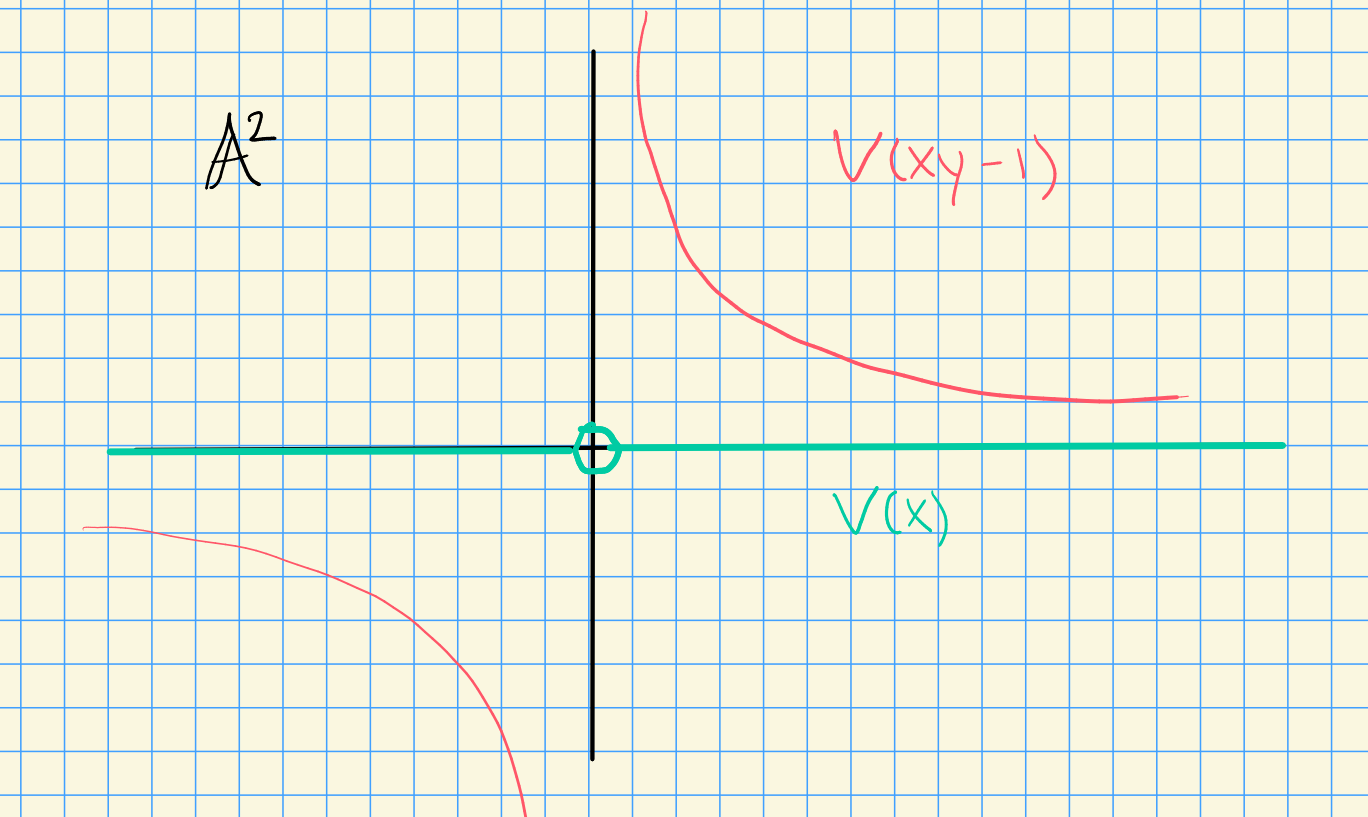
\includegraphics{figures/image_2020-10-15-09-50-03.png}
\caption{Image}
\end{figure}

Note that \(\pi: X\cross \AA^1 \to X\) is regular, using prop 3.8: if
the coordinates of a map are regular functions, then the entire map is a
morphism of ringed spaces. We can then note that \(1\over f(x)\) is
regular on \(D(f)\), since \(f\neq 0\) there.

\end{proof}

\begin{example}

\(\AA^2 \smz\) is not an affine variety. Note that this is also not a
distinguished open.

We showed on a HW problem that the regular functions on \(\AA^2\smz\)
are \(k[x, y]\), which are also the regular functions on \(\AA^2\). So
there is a map inducing a pullback
\begin{align*}  
\iota: \AA^2\smz &\to \AA^2 \\
\iota^* k[x, y] \mapsvia{\sim} k[x, y]
.\end{align*} Note that \(\iota^*\) is an isomorphism on the space of
regular functions, but \(\iota\) itself is not an isomorphism of
topological spaces. Why? \(i^{-1}\) is not defined at zero.

\end{example}

\hypertarget{chapter-5}{%
\subsection{Chapter 5}\label{chapter-5}}

\begin{definition}[Prevariety]

A \emph{prevariety} is a ringed spaced \(X\) with a finite open cover by
affine varieties. This is a topological space \(X\) with an open cover
\(\ts{U_i}_{i=1}^n \covers X\) such that \((U_i, \ro{\OO_X}{U_i} )\) is
isomorphic to an affine variety. We'll call \(\OO_X\) the sheaf of
\emph{regular functions} and \(U_i\subset X\) \emph{affine open sets}.

\end{definition}

One way to construct prevarieties from affine varieties is by
\emph{gluing}:

\begin{definition}[Glued Spaces]

let \(X_1, X_2\) be prevarieties which are themselves actual varieties.
Let \(U_{12} \subset X_1, U_{21} \subset X_2\) be opens and
\(f: U_{12} \to U_{21}\) an isomorphism of ringed spaces.

\begin{figure}
\centering
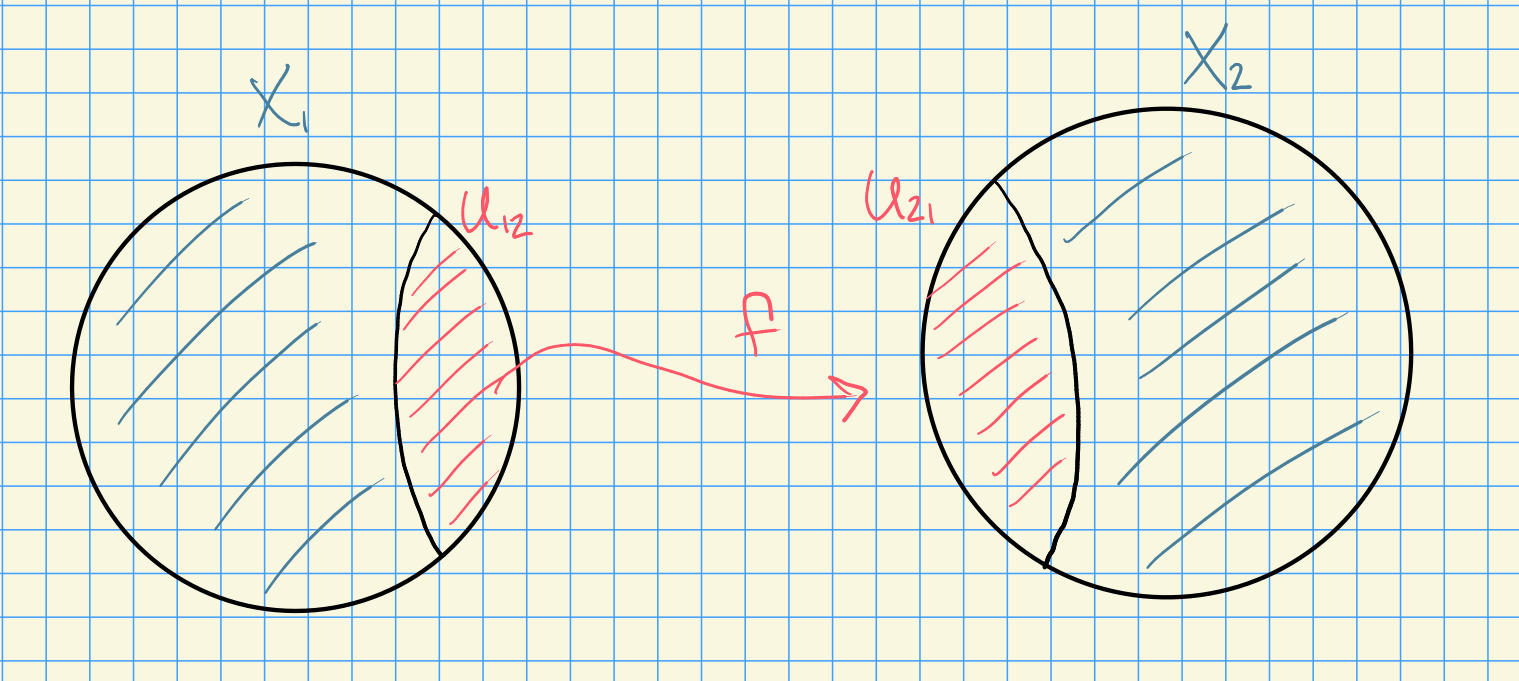
\includegraphics{figures/image_2020-10-15-10-08-59.png}
\caption{Image}
\end{figure}

As a set, take \(X = X_1 \disjoint X_2/\sim\) where \(a\sim f(a)\) for
all \(a\in U_{12}\). As a topological space, \(U \subset X\) is open iff
\(U_i \da U\intersect X_i\) are open in \(X_i\). As a ringed space, we
take
\(\OO_X(U) \da \ts{\phi: U\to k \st \ro{\phi}{U_i} \in \OO_{X_i}}\).

\end{definition}

\begin{example}

The prototypical example is \(\PP^1/k\) constructed from two copies of
\(\AA^1/k\). Set \(X_1 = \AA^1, X_2 = \AA^2\), with
\(U_{12} \da D(x) \subset X_1\) and \(U_{21} \da D(y) \subset X_2\).
Then let
\begin{align*}  
f: U_{12} &\to U_{21} \\
x & \mapsto {1\over x}
.\end{align*} This defines a regular function on \(U_{12}\) so defines a
morphism \(U_{12} \mapsvia{\sim} \AA^1\).

\begin{figure}
\centering
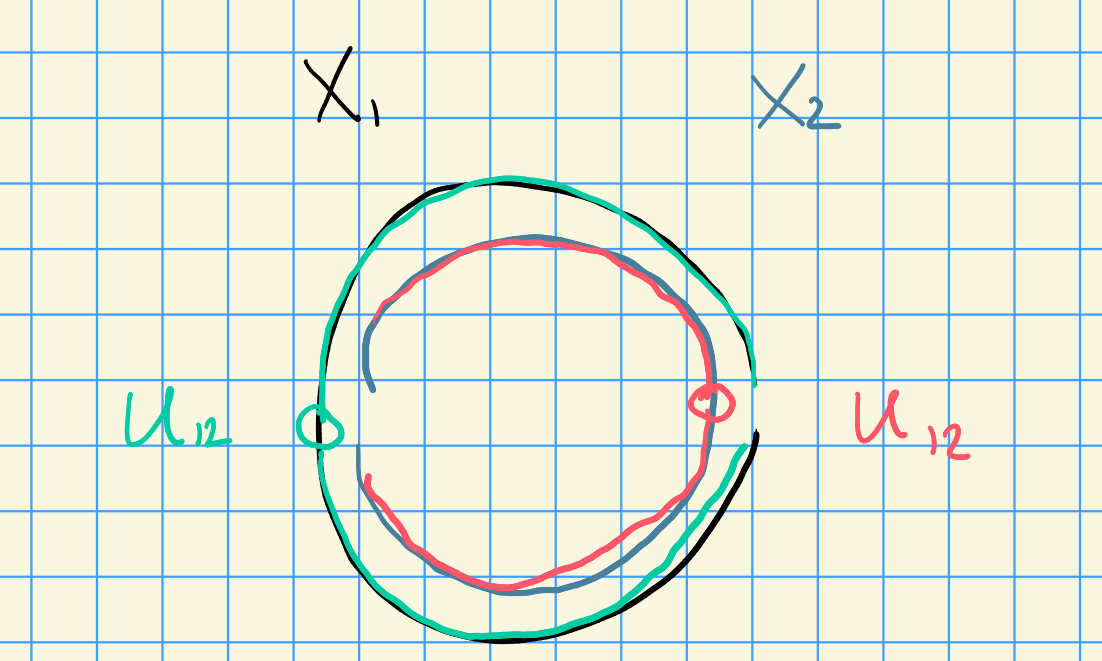
\includegraphics{figures/image_2020-10-15-10-20-32.png}
\caption{Image}
\end{figure}

Over \(\CC\), topologically this yields a sphere

\begin{figure}
\centering
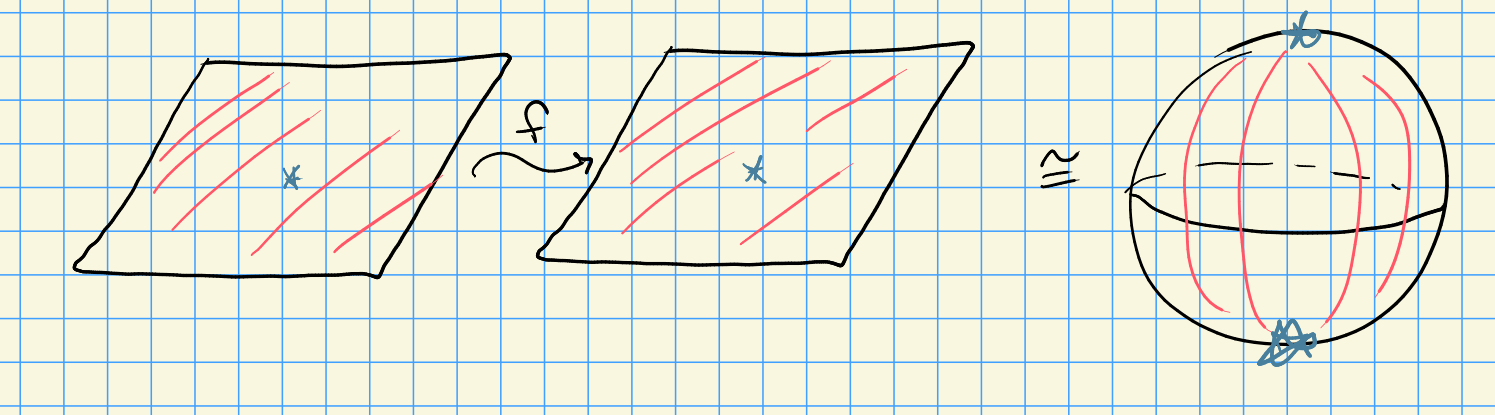
\includegraphics{figures/image_2020-10-15-10-23-24.png}
\caption{Image}
\end{figure}

Given a ringed space \(X = X_1\union X_2\) with a structure sheaf
\(\OO_X\), what is \(\OO_X(X)\)? By definition, it's

\begin{align*}  
\OO_X(X) \da \ts{\phi: X\to k \st \ro{\phi}{X_1}, \ro{\phi}{X_2} \text{ are regular} }
.\end{align*}

Then if \(\ro{\phi}{X_1} = f(x)\) and \(\ro{\phi}{X_2} = g(y)\), we have
\(y=1/x\) on the overlap and so \(\ro{f(x)}{D(x)} = \ro{g(1/x)}{D(x)}\).
Since \(f, g\) are rational functions agreeing on an infinite set,
\(f(x) = g(1/x)\) both being polynomial forces \(f = g = c\) for some
constant \(c \in k\). Thus \(\OO_X(X) = k\).

What about \(\OO_X(X_1)\)? This is just \(k[x]\), and similarly
\(\OO_X(X_2) = k[y]\). We can also consider
\(\OO_X(X_1\intersect X_2) = D(x) \subset X\), so this yields
\(k[x, 1/x]\). We thus have a diagram

\begin{center}
\begin{tikzcd}
                         & \OO_X(X_1) = k[x] \ar[rd, "x\mapsto x"]   & \\
\OO_X(X) \ar[ru] \ar[rd] &                                           & \OO_X(X_1\intersect X_2) = k[x, 1/x] \\
                         & \OO_X(X_2) = k[y] \ar[ru, "y\mapsto 1/x"] &
\end{tikzcd}
\end{center}

\end{example}

\hypertarget{tuesday-october-20}{%
\section{Tuesday, October 20}\label{tuesday-october-20}}

\hypertarget{gluing-two-opens}{%
\subsection{Gluing Two Opens}\label{gluing-two-opens}}

Recall that a \emph{prevariety} is a ringed space that is locally
isomorphic to an affine variety, where we recall that \((X, \OO_X)\) is
\emph{locally isomorphic} to an affine variety iff there exists an open
cover \(U_i \covers X\) such that \((U_i, \OO_{U_i})\).

We found one way of producing these: the gluing construction. Given two
ringed spaces \((X_1, \OO_{X_1})\) and \((X_2, \OO_{X_2})\) and open
sets \(U_{12} \in X_1\) and \(U_{21} \in X_2\) and an isomorphism
\((U_{12}, \OO_{U_{12}}) \mapsvia{f} (U_{21}, \OO_{U_{21}})\), we
defined

\begin{itemize}
\tightlist
\item
  The topological space as \(X_1 \disjoint_f X_2\)
\item
  The sheaf of rings as
  \(\OO_X = \ts{\phi:U\to k \st\ro{\phi}{U\intersect X_i} \text{ is regular for } i=1,2 }\).
\end{itemize}

\begin{example}

\(\PP^1/k = X_1 \union X_2\) where \(X_1 \cong \AA^1, X_2 \cong \AA^2\).
Take \(U_{12} = D(x)\) and \(U_{21} = D(y)\) with
\begin{align*}  
f: U_{12} &\to U_{21} \\
x &\mapsto {1\over x} = y
.\end{align*}

\begin{figure}
\centering
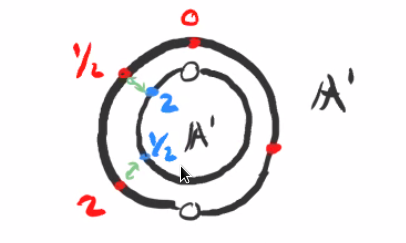
\includegraphics{figures/image_2020-10-20-09-41-55.png}
\caption{Supposing \(\ch(k) \neq 2\). Note that for \(\CC\) this
recovers \(S^2\) in the classical topology.}
\end{figure}

\end{example}

\begin{example}

Let \(X_i = \AA^1\) and \(U_{12} = D(x), U_{21} = D(y)\) with
\begin{align*}  
f: U_{12} &\to U_{21} \\
x &\mapsto x=y
.\end{align*}

\begin{figure}
\centering
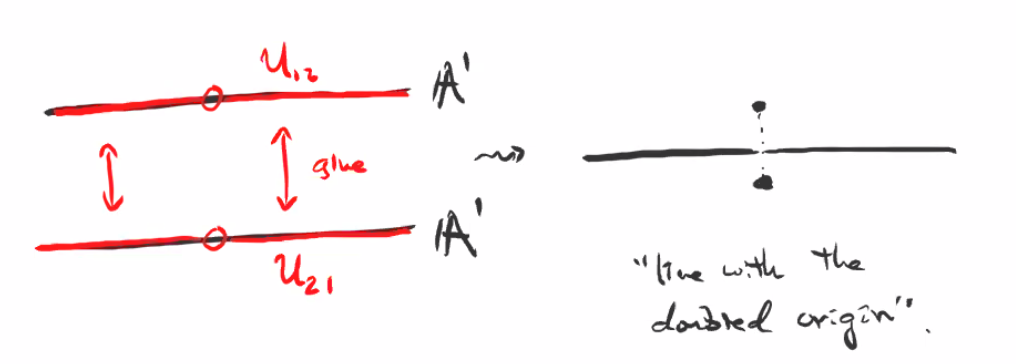
\includegraphics{figures/image_2020-10-20-09-44-41.png}
\caption{Line with the doubled origin.}
\end{figure}

Then
\(\OO_X = \ts{\phi: X\to k \st \ro{\phi}{X_i} \text{ is regular}} \cong k[x]\).

\end{example}

\hypertarget{more-general-gluing}{%
\subsection{More General Gluing}\label{more-general-gluing}}

Now we want to glue more than two open sets. Let \(I\) be an indexing
set for prevarieties \(X_i\). Suppose that for an ordered pair
\((i, j)\) we have open sets \(U_{ij} \subset X_i\) and isomorphisms
\(f_{ij}: U_{ij} \mapsvia{\sim} U_{ji}\) such that

\begin{enumerate}
\def\labelenumi{\alph{enumi}.}
\item
  \(f_{ji} = f_{ij}^{-1}\)
\item
  \(f_{jk} \circ f_{ij} = f_{ik}\) (cocycle condition)
\end{enumerate}

\begin{figure}
\centering
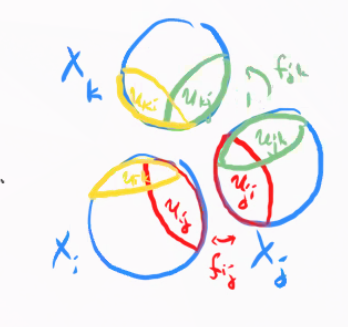
\includegraphics{figures/image_2020-10-20-09-54-14.png}
\caption{Opens with isomorphisms.}
\end{figure}

Then the gluing construction is given by

\begin{enumerate}
\def\labelenumi{\arabic{enumi}.}
\item
  \(X\da \disjoint X_i/\sim\) where \(x\sim f_{ij}(x)\) for all \(i,j\)
  and all \(x\in U_{ij}\).
\item
  \(\OO_x(U) \da \ts{\phi:U\to k \st \ro{\phi}{U\intersect X_i} \in \OO_{X_i} }\).
\end{enumerate}

Every prevariety arises from the gluing construction applied to \(X_i\)
affine varieties, since a prevariety \((X, \OO_X)\) by definition has an
open affine cover \(X_i \covers X\) and \(X\) is the result of gluing
the \(X_i\)s by the identity.

\begin{example}

Let \(X_1 = X_2 = X_3 = \AA^2/k\). Glue by the following instructions:

\begin{figure}
\centering
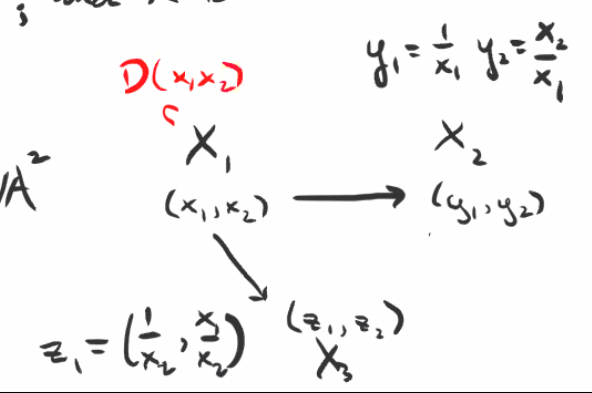
\includegraphics{figures/image_2020-10-20-10-11-07.png}
\caption{The map not shown is whatever formula is necessary to make the
diagram commute.}
\end{figure}

Here

\begin{itemize}
\tightlist
\item
  \((y_1, y_2) = (1/x_1, x_2/x_1)\)
\item
  \((z_1, z_2) = (1/x_2, x_1/x_2)\)
\item
  \(U_{12} = D(x_1)\)
\item
  \(U_{21} = D(x_2)\).
\end{itemize}

\begin{figure}
\centering
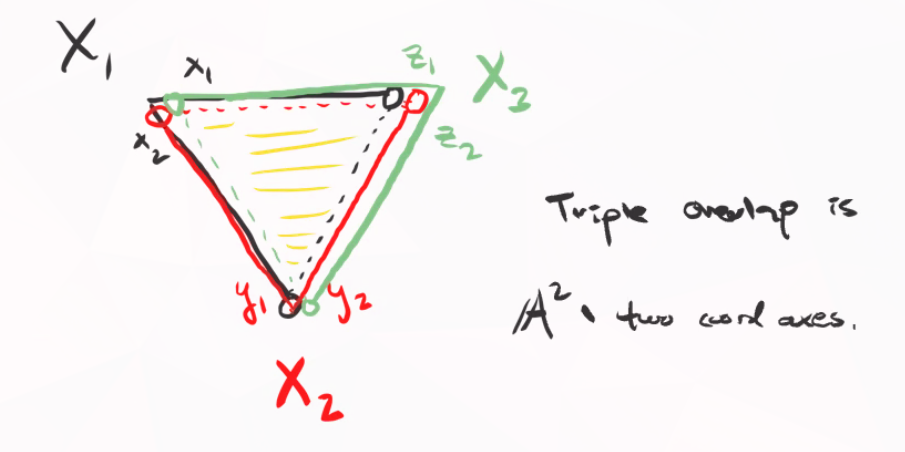
\includegraphics{figures/image_2020-10-20-10-13-56.png}
\caption{Yields \(\PP^2\)}
\end{figure}

Here \(X_1 = [1: y/x: z/x]\), \(X_2 = [x/y: 1: z/y]\).

\end{example}

\begin{example}

From Gathmann 5.10, open and closed subprevarieties. Let \(X\) be a
prevariety and suppose \(U\subset X\) is open. Then \((U, \OO_U)\) is a
prevariety where \(\OO_U = \ro{\OO_X}{U}\). How can we write \(U\) as
(locally) an affine variety?

Since the \(U_i\) are covered by distinguished opens \(D_{ij}\) in
\(X_i\) where \(X = \union X_i\) with \(X_i\) affine varieties, we can
write \(U = \Union_i U_i = \Union_{i, j} D_{ij}\).

\end{example}

\begin{example}

Let \(Y\subset X\) be a closed subset of a prevariety \(X\). We need to
define \(\OO_Y(U)\) for all \(U\subset Y\) open, so we set
\begin{align*}  
\OO_Y(U) = \ts{\phi: U\to k \st \forall p\in U, \, \exists V_p \text{ with } p\in V_p \subset_{\text{open}} X \text{ and } \psi\in \OO_X(V_p) \text{ s.t. } \ro{\psi}{U\intersect V} \phi  }
.\end{align*}

What's the picture?

\begin{figure}
\centering
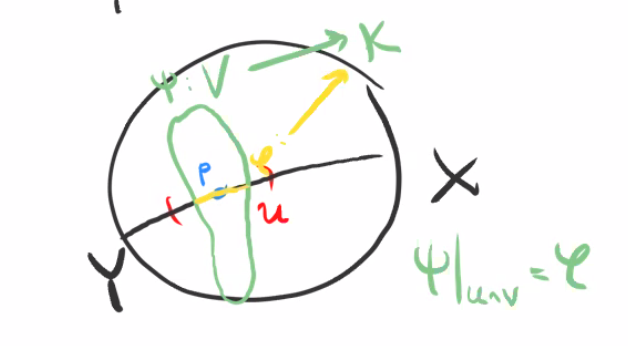
\includegraphics{figures/image_2020-10-20-10-29-25.png}
\caption{Sheaf for a closed subset.}
\end{figure}

It's an exercise to show that this is a prevariety.

\end{example}

\begin{remark}

If \(U\subset X\) is an open subprevariety or \(Y\subset X\) is a closed
subprevariety, then the inclusions are morphisms. We'd need to show that
a pullback of a function is regular, but this is set up by definition.

\end{remark}

\begin{remark}

Define \(\tilde \OO_X(U)\) as the set of \emph{all} functions
\(U\to k\). Then the inclusion \((X, \OO_X) \injects (X, \tilde \OO_X)\)
given by the identity on \(X\) is a morphism, but the identity in the
reverse direction is not.

\end{remark}

\hypertarget{thursday-october-22}{%
\section{Thursday, October 22}\label{thursday-october-22}}

\begin{example}

Consider \(\AA^1\), whose polynomial functions are \(k[x]\). Consider
now \(D(x) \subset \AA^1\), which is equal to the affine variety
\(V(xy-1)\). Then the polynomial functions on \(D(x)\) are
\(k[x, y] / \gens{xy-1} \cong k[x, x^{-1} ]\).

\end{example}

Recall that a \emph{prevariety} is a ringed space \((X, \OO_X)\) such
that \(X\) has a finite open cover by affine varieties
\((U_i, \ro{\OO_X}{U_i})\), and a \emph{morphism} of prevarieties is a
morphism of ringed spaces. We saw that one can construct prevarieties by
gluing finite collections of prevarieties or affine varieties along open
sets, and all prevarieties arise this way.

Similar to varieties, the product \(P\) of prevarieties \(X, Y\) will
satisfy a universal property:

\href{https://tikzcd.yichuanshen.de/\#N4Igdg9gJgpgziAXAbVABwnAlgFyxMJZABgBpiBdUkANwEMAbAVxiRAAUQBfU9TXfIRQBGUsKq1GLNgC1uvEBmx4CRAExiJ9Zq0QgAGvL7LBRUWq1TdIAJrcJMKAHN4RUADMAThAC2SUSA4EEgAzDwe3n6IAUFIauEgXr7+1LGIZCAMWGDWUHRwABaOINTa0noAOhUwAB5YcDgICUlRGWkaIABGMGBQoRll1lVoWAD6hs2RSG3BiCHU3b1IALQhA1Zsw2N21Ax03Qzs-CpCIJ5YTgU49lxAA}{Tikz
Link}

\begin{center}
\begin{tikzcd}
P \arrow[rrd, "\pi_X", bend left] \arrow[rdd, "\pi_Y"', bend right] &                                                     &   \\
                                                                    & Z \arrow[d] \arrow[r] \arrow[lu, "\exists !", dashed] & X \\
                                                                    & Y                                                   &  
\end{tikzcd}
\end{center}

\begin{proposition}[?]

The product is unique up to unique isomorphism, i.e.~there is a unique
isomorphism between any two products.

\end{proposition}

\begin{proof}

Standard!

\end{proof}

\begin{example}

Consider \(\AA^1 \times \AA^1\), then the product is (and should be)
\(\AA^2\), but \(\AA^2\) does not have the product topology. The open
set \(D(x-y)\) is not covered by products of open sets.

\begin{quote}
This happens because the Zariski topology is too weak.
\end{quote}

\end{example}

Strategy to fix: use gluing. Let \(X, Y\) be prevarieties and
\(\ts{U_i}, \ts{V_i}\) be open affine covers of \(X\) and \(Y\)
respectively. We can construct the product
\(U_i \cross V_j \subset \AA^{n+m}\), which is an affine variety and
satisfies the universal property for products. We then glue two such
products \(U_{i_1} \cross V_{j_1}\) and \(U_{i_2} \cross V_{j_2}\) along
their common open subset in
\(\qty{U_{i_1}\cap U_{i_2} }\intersect\qty{V_{j_1} \cap V_{j_2}} \subseteq X\cross Y\).

Let
\(\tilde U \da U_{i_1} \intersect U_{i_2} \cross V_{j_1} \intersect V_{j_2}\),
we then need that

\begin{align*}  
(\tilde U, \ro{ \OO_{U_{i_1} \cross V_{j_1}} }{\tilde U} ) \cong
(\tilde U, \ro{ \OO_{U_{i_2} \cross V_{j_2}} }{\tilde U} )
.\end{align*} This follows from the universal property of products,
since the open set \((U\cross V, \ro{ \OO_{X\cross Y} }{U\cross V} )\)
is a categorical product of ringed spaces, and the identity provides a
unique isomorphism. By the gluing construction, this produces a ringed
space \((X\cross Y, \OO_{X\cross Y})\), we just need to check that this
satisfies the universal property. We have projections \(\pi_X, \pi_Y\)
set-theoretically, which restrict to morphisms on every
\(U_i \cross V_j\). For any prevariety \(Z\), we get a unique set map
\(h:Z\to X\cross Y\) which commutes, so it suffices to check that \(h\)
is a morphism of ringed spaces.

So consider \(h^{-1} (U_i \cross V_j) \subset Z\), which is an open
subset of \(Z\) given by \(f^{-1}(U) \cross f^{-1}(V)\). Take an open
cover and let \(W\) be an element in it. We can then restrict \(f\) and
\(g\) to get \(\ro{f}{W}:W\to U_i\) and \(\ro{g}{W}:W\to V_j\) and their
product is a morphism of ringed spaces. So \(Z\) is covered by open sets
for which \(h\) is a morphism of ringed spaces, making \(h\) itself a
morphism.

What was the point of constructing the product? We want some notion
analogous to being Hausdorff to distinguish spaces like \(\PP^1/k\) from
the line with the doubled origin. The issue is that these spaces with
the Zariski topology are never Hausdorff. So we make the following
definition:

\begin{definition}[Separated]

A prevariety is \textbf{separated} iff
\(X \injectsvia{\Delta_X} X\cross X\) is a closed embedding, where
\(\Delta(x) = (x, x)\) is the diagonal morphism.
i.e.~\(\id_X \cross \id_X\).

\end{definition}

\begin{definition}[Variety]

A \textbf{variety} is a separated prevariety.

\end{definition}

\hypertarget{tuesday-october-27}{%
\section{Tuesday, October 27}\label{tuesday-october-27}}

Recall that an affine variety is given by \(X = V(I) \subset \AA^n/k\),
and we have sheaves of rings of regular functions \(\OO_X\) on \(X\). A
prevariety is a ringed space that is covered by finitely many affine
spaces. A morphism of prevarieties \(f:X\to Y\) is a continuous map such
that the pullbacks of regular functions are regular, i.e.~for all
\(\phi \in \OO_X(U)\) we have \(f^* \phi \in \OO_X(f^{-1} (U) )\). We
can form a category \(\operatorname{PreVar}_k\) of prevarieties over
\(k\), where we have several important constructions

\begin{enumerate}
\def\labelenumi{\arabic{enumi}.}
\item
  Gluing
\item
  Products: Given \(X, Y\), there is a unique prevariety \(X\cross Y\)
  such that

  \begin{center}
  \begin{tikzcd}
    Z\ar[drr, bend left , "f_x"] \ar[rdd, bend right, "f_y"] \ar[rd, "\exists ! h", dotted] &                                         & \\
                                                                                         & X\cross Y\ar[r, "\pi_X"]\ar[d, "\pi_Y"] & X \\
                                                                                         & Y                                       &
    \end{tikzcd}
  \end{center}
\end{enumerate}

We had an analogue of being Hausdorff: the diagonal \(\Delta_X\) is
closed.

\begin{example}

Glue \(D(x) \subset \AA^1\) to \(D(y) \subset \AA^1\) by the isomorphism
\begin{align*}  
D(x) & \mapsvia{\sim} D(y) \\
x &\mapsto y
.\end{align*} This yields an affine line with two origins:

\begin{figure}
\centering
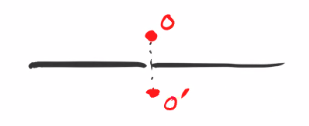
\includegraphics[width=2.60417in,height=\textheight]{figures/image_2020-10-27-09-47-27.png}
\caption{Line with two origins.}
\end{figure}

Consider the product:

\begin{figure}
\centering
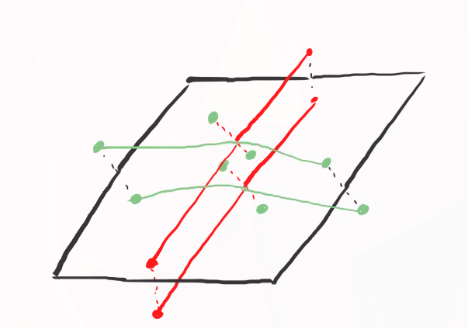
\includegraphics[width=2.60417in,height=\textheight]{figures/image_2020-10-27-09-51-10.png}
\caption{Product of lines with two origins}
\end{figure}

Since the diagonal is given by \(\Delta_X = \ts{(x, x) \st x\in X}\), we
have the following situation in blue:

\begin{figure}
\centering
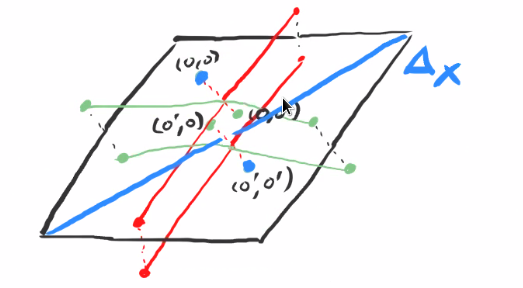
\includegraphics[width=2.60417in,height=\textheight]{figures/image_2020-10-27-09-52-26.png}
\caption{Image}
\end{figure}

We claim that \(\Delta_X\) is not closed, and for example
\((0, 0') \in \bar{\Delta}_X\). Consider
\(U\cross U' \subset X\cross X\) where \(U, U'\) are the two copies of
\(\AA^1\) in \(X\). This is an affine open set, since it's isomorphic to
\(\AA^1\cross \AA^1\).

If \(\Delta_X\) were closed, then
\(S \da \Delta_X \intersect (U\cross U') = \ts{(x, x) \st x\neq 0}\)
would be closed in \(U\cross U'\).

\begin{figure}
\centering
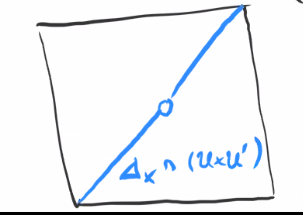
\includegraphics[width=2.60417in,height=\textheight]{figures/image_2020-10-27-10-01-15.png}
\caption{Open diagonal in a product.}
\end{figure}

This is because any polynomial vanishing on \(S\) must vanish at
\((0, 0)\), so \(S\) is an affine variety. But then
\(V(I(S)) = \Delta_{\AA^1}\).

\end{example}

\begin{lemma}[?]

\envlist

\begin{enumerate}
\def\labelenumi{\alph{enumi}.}
\item
  Any affine variety is a variety.
\item
  Open and closed subprevarieties of a variety \(X\) are themselves
  varieties.
\end{enumerate}

Thus it makes since to consider \emph{open} and \emph{closed
subvarieties}.

\end{lemma}

\begin{proof}[of a]

We need to check that \(\Delta_X \subset X^2\) is closed for any affine
\(X\subset \AA^n\). Note that we can write.
\begin{align*}
\Delta_X = X^2 \intersect V\qty{ \ts{x_j - y_j \st 1\leq j \leq n}} \subset \AA^n \cross \AA^2
\end{align*}

\end{proof}

\begin{proof}[of b]

Let \(\iota:Y\to X\) be the inclusion of either an open or closed
subset. Then we have a morphism \((\iota, \iota): Y^2 \to X^2\) by the
universal property. Then \(\Delta_Y = (\iota, \iota)^{-1} (\Delta_X)\),
so is closed by the continuity of \((\iota, \iota)\) and the fact that
\(\Delta_X\). Thus \(Y\) is a variety.

\end{proof}

\hypertarget{properties-of-varieties}{%
\subsection{Properties of Varieties}\label{properties-of-varieties}}

\begin{proposition}[Properties of Varieties]

Let \(f, g: X\to Y\) be morphisms of prevarieties and assume \(Y\) is a
variety.

\begin{enumerate}
\def\labelenumi{\alph{enumi}.}
\item
  The graph of \(f\), given by
  \(\Gamma_f \da \ts{(x, f(x)) \st x\in X}\), is closed in
  \(X\cross Y\).
\item
  The set \(\ts{x\in X\st f(x) = g(x)}\) is closed in \(X\).
\end{enumerate}

\end{proposition}

\begin{proof}[of a]

Consider the product morphism \((f, \id): X\cross Y \to Y^2\). Since
\(\Delta_Y\) is closed, \((f, \id)^{-1} (\Delta_Y)\) is closed, and is
the locus where \(f(x) = y\), so this is \(\Gamma_f\).

\end{proof}

\begin{proof}[of b]

Consider \((f, g): X\to Y^2\). Since \(\Delta_Y \subset Y^2\) is closed,
\begin{align*}
(f, g)^{-1}(\Delta_Y) = \ts{x\in X \st f(x) = g(x)} \subset X
\end{align*}

is closed.

\end{proof}

\hypertarget{chapter-6-projective-varieties}{%
\subsection{Chapter 6: Projective
Varieties}\label{chapter-6-projective-varieties}}

Note that affine varieties of positive dimension over \(\CC\) are not
compact in the classical topology, but \emph{are} compact in the Zariski
topology. Similarly, they are Hausdorff classically, but not in the
Zariski topology. We want to find notions equivalent to Hausdorffness
and compactness in the classical setting, which end up also applying to
varieties. The fix in the latter case was considering ``separatedness''.
:q The fix for compactness will be the following:

\begin{definition}[Complete]

A variety \(X\) is \textbf{complete} iff for any variety \(Y\) the
projection map \(\pi_Y:X\cross Y\to Y\) is a closed map,
i.e.~\(\pi_Y(U)\) is closed whenever \(U\) is closed.

\end{definition}

\begin{example}

\(\AA^1\) is not complete. Let \(Y=\AA^1\) and
\(Z = V(xy-1)\subset X\cross Y\). Then
\(\pi_Y(Z) = D(y) \subset Y \subset \AA^1\) is not closed.

\end{example}

\hypertarget{thursday-october-29}{%
\section{Thursday, October 29}\label{thursday-october-29}}

\hypertarget{projective-space}{%
\subsection{Projective Space}\label{projective-space}}

\begin{definition}[Projective Space]

Let \(n\in \NN\), and define \textbf{projective \(n\dash\)space} over
\(k\) by\\
\begin{align*}  
\PP^n/k = \ts{\text{lines through the origin in } k^{n+1}}
.\end{align*}

\end{definition}

\begin{remark}

For notation, given \(L\in \PP^n/k\), it is spanned by any nonzero
points \(\tv{x_0, \cdots, x_n} \in L\), and \(L\) is uniquely determined
by this point up to scaling by elements in \(k\units\). In this case, we
write
\(L = \tv{x_0: \cdots : x_n} = \tv{\lambda x_0: \cdots : \lambda x_n}\).
We can then define \(\PP^n/k = k^{n+1}\smz / \sim\) where we mod out by
scalar multiplication. We call \([x_1 : \cdots : x_n]\) the
\emph{homogeneous coordinates} on \(\PP^n/k\).

\end{remark}

\begin{remark}

Consider the map
\begin{align*}  
\AA^n \to \PP^n \\
\tv{x_1, \cdots, x_n} &\mapsto \tv{1: x_1 : \cdots : x_n}
.\end{align*} This is injective. Conversely, consider
\begin{align*}  
"D(x_0)" \subset \PP^n \da \ts{\tv{x_0 : \cdots : x_n} \st x_0\neq 0}
.\end{align*} This is a well-defined subset of \(\PP^n\), since it only
depends on the equivalence class of a point. In this case, there is a
unique \(\lambda(x_0, \cdots, x_n)\), namely \(\lambda = 1/x_0\), such
that each point in this set is of the form
\(\tv{1: {x_1\over x_0} : \cdots : {x_n \over x_0}}\), yielding a copy
of \(\AA^n\subset \PP^n\) given by points
\(\tv{{x_1\over x_0}, \cdots, {x_n\over x_0}}\). What is its complement?

It's given by \(\ts{\tv{0: x_1: \cdots : x_n}} \subset \PP^n\), which is
equal (as a set) to a copy of \(\PP^{n-1}\) defined by the set of lines
in \(k^n\) defined by \(x_0 = 0\).

\end{remark}

\begin{example}[?]

Note that \(\PP^1\) contains a copy of \(\AA^1\) where \(x_0 \neq 0\)
and a second copy where \(x_1 \neq 0\), admitting maps
\begin{align*}  
f_1: \AA^1 &\to \PP^1 \\
\tv{x_0: x_1} &\mapsto \tv{{x_0 \over x_1}}
.\end{align*}

and

\begin{align*}  
f_2: \AA^1 &\to \PP^1 \\
\tv{x_0: x_1} &\mapsto \tv{{x_1 \over x_0}}
,\end{align*} since every line in \(\PP^1\) has either \(x_0\neq 0\) or
\(x_1 \neq 0\). These two copies cover \(\PP^1\), and the ``transition
map'' is inversion.

\end{example}

\begin{remark}

More generally, there are \(n+1\) inclusions \(\AA^n \injects \PP^n\)
given by dividing by the \(j\)th coordinate, and their union is the
entire space. The gluing construction gives \(\PP^n\) the structure of a
prevariety: we can consider \(D(x_j) \subset \PP^n\) where each has the
structure of a ringed space \((\AA^n, \OO_{\AA^n})\). We have
\(D(x_i) \intersect D(x_j) \subset D(x_i)\) is given coordinate
\(x_k/x_i\) where \(k\neq i\), and similarly this is a subset of
\(D(x_j)\) with coordinates \(x_k/x_j\) for \(k\neq j\). Their
intersection is \(D({x_i \over x_j})\), which is a copy of
\(\AA^{n-1}\).

\end{remark}

\begin{example}[?]

Consider \(\PP^1\), then \(D(x_0) \cong \AA^1\) with which contains a
copy of \(\AA^1\) with coordinate ring \(k\tv{{x_1\over x_0}}\) and a
subset \(D\qty{x_1\over x_0}\) with coordinate ring \(k[y, 1/y]\), and
similarly, \(D(x_1) \cong \AA^1\) has coordinate ring
\(k\tv{{x_0\over x_1}}\) and contains \(\contains D\qty{x_0\over x_1}\)
with coordinate ring \(k[z, 1\over z]\). Consider their overlap
\(D(x_0) \intersect D(x_1)\)? When do \(y, z\) denote the same point in
\(\PP^1\)? When \(y = 1/z\).

We can conclude that the \(n+1\) copies \(D(x_i) \subset \PP^n\) are
affine varieties isomorphic as ringed spaces on the overlaps, so the
gluing construction makes \(\PP^n\) a prevariety.

\end{example}

\begin{definition}[Homogeneous Polynomial]

A polynomial \(f\) is homogeneous of degree \(f\) is every monomial in
\(f\) has total degree \(d\).

\end{definition}

\begin{example}[?]

\begin{figure}
\centering
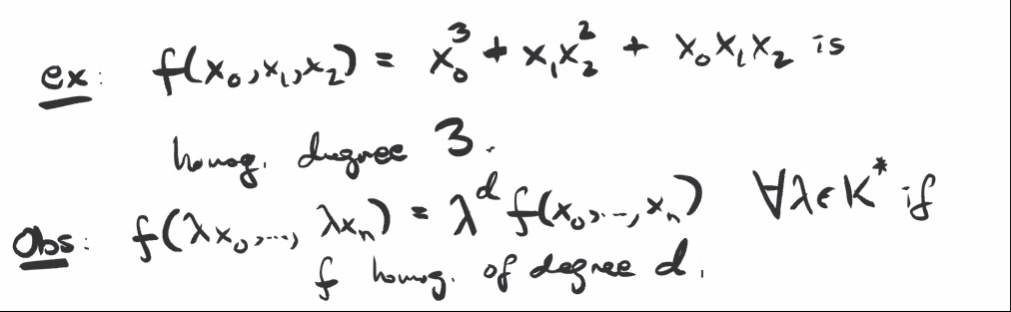
\includegraphics{figures/image_2020-10-29-10-29-48.png}
\caption{Image}
\end{figure}

\end{example}

If \(f\) is homogeneous, \(V(f) \subset \PP^n\) is a well-defined
subset, since
\(f(x_0, \cdots, x_n) = 0 \iff \lambda^d f(x_0, \cdots, x_n) = 0 \iff f(\lambda x_0, \cdots, \lambda x_n) = 0\).

\begin{definition}[?]

A graded ring \(R\) is a ring \(R\) with abelian subgroups
\(R_d \subset R\) with \(R = \bigoplus_{d\geq 0} R_d\) and for all
\(f\in R_d\) and \(g\in R_{d'}\), we have \(fg \in R_{d+d'}\) and
\(R_d + R_{d} \subset R_d\).

\end{definition}

\hypertarget{thursday-november-05}{%
\section{Thursday, November 05}\label{thursday-november-05}}

Today: projective spaces. We defined
\(\PP^n_{/k} \da k^{n+1}\smz /\sim\) where \(x\sim \lambda x\) for all
\(x\in k\units\), which we identified with lines through the origin in
\(k^{n+1}\). We have homogeneous coordinates
\(p = [x_0: \cdots : x_n]\).

We say an ideal is \emph{homogeneous} iff for all \(f\in I\), the
homogeneous part \(f_d\in I\) for all \(d\). In this case
\(V_p(I) \subset \PP^{n}_{/k}\) defined as the vanishing locus of all
homogeneous elements of \(I\) is well-defined. Think of this as the
``projective version'' of a vanishing locus.

Similarly we defined \(I_p(S)\) defined as the ideal generated by all
homogeneous \(f\in \kx{n}\) such that \(f(x) = 0\) for all \(x\in S\).

\begin{remark}

Observe that \(V_a(I)\) defined as the cone over \(V_p(I)\) is the set
of points in \(\AA^{n+1}\smz \union \ts{0}\) which map to \(V_p(I)\).

\end{remark}

We have an alternative definition of a cone in \(\AA^{n+1}\),
characterized as a closed subset \(C\) which is closed under scaling, so
\(kC\subseteq C\).

\begin{proposition}

\envlist

\begin{itemize}
\item
  If \(S\subset \kx{n}\) is a set of homogeneous polynomials, then
  \(V_a(S)\) is a cone since it is closed and closed under scaling. This
  follows from the fact that \(f(x) = 0 \iff f(\lambda x) = 0\) for
  \(\lambda \in k\units\) when \(f\) is homogeneous.
\item
  If \(C\) is a cone, then its affine ideal \(I_a(C)\) is homogeneous.
\end{itemize}

\end{proposition}

\begin{proof}[?]

Let \(f\in I_a(C)\), then \(f(x) = 0\) for all \(x\in C\). Since \(C\)
is closed under scaling, \(f(\lambda x) = 0\) for all \(x\in C\) and
\(\lambda \in k\units\). Decompose \(f = \sum_d f_d\) into homogeneous
pieces, then
\begin{align*}  
x\in C \implies 0 = f(\lambda x) = \sum \lambda^d f_d(x) 
.\end{align*}

Fixing \(x\in C\), the quantities \(f_d(x)\) are constants, so the
resulting polynomial in \(\lambda\) vanishes for all \(\lambda\). But
since \(k\) is infinite, this forces \(f_d(x) = 0\) for all \(d\), which
shows that \(f_d \in I_a(C)\).

\end{proof}

\begin{lemma}[?]

There is a bijective correspondence
\begin{align*}  
\correspond{\text{Cones}} 
&\iff
\correspond{\text{Projective Varieties}} \\
\AA^{n+1} \supset X &\mapsto \PP X\subset \PP^n \\
\AA^{n+1} \supset CX &\mapsfrom X\subset \PP^n \\
.\end{align*}

\end{lemma}

\begin{proof}[?]

\(\PP V_a(S) = V_p(S)\) for any set \(S\) of homogeneous polynomials,
and \(C(V_p(S)) = V_a(S)\), where \(V_p(S)\) is a cone by part (a) of
the previous proposition. Conversely, every cone is the variety
associated to some homogeneous ideal.

\end{proof}

\hypertarget{projective-nullstellensatz}{%
\subsection{Projective
Nullstellensatz}\label{projective-nullstellensatz}}

\begin{definition}[Irrelevant Ideal]

The homogeneous ideal \(I_0 \da (x_0, \cdots, x_n) \subset \kx{n}\) is
denoted the \textbf{irrelevant ideal}.

\end{definition}

\begin{proposition}[Projective Nullstellensatz]

\envlist

\begin{enumerate}
\def\labelenumi{\alph{enumi}.}
\item
  For all \(X\subseteq \PP^n\), \(V_p(I_p(X)) = X\).
\item
  For all homogeneous ideal \(J\subset \kx{n}\) such that (importantly)
  \(\sqrt{J} \neq I_0\), \(I_p(V_p(J)) = \sqrt J\).
\end{enumerate}

\end{proposition}

\begin{proof}[of a]

\(\supset\): If we let \(I\) denote the ideal of all homogeneous
polynomials vanishing on \(X\), then this certainly contains \(X\).

\(\subset\): This follows from part (b), since \(X = V_p(J)\) implies
that \((V_p I_p V_p)(J) = V_p(\sqrt J) = V_p(J) = X\), since taking
roots of homogeneous polynomials doesn't change the vanishing locus.

\end{proof}

\begin{proof}[of b]

That \(I_p(V_p(J)) \supset \sqrt J\) is obvious, since \(f\in \sqrt{J}\)
vanishes on \(V_p(J)\). \todo[inline]{Check}

It remains to show \(\sqrt{J} \subset I_p(V_p(J))\) , but we can write
\(I_p(V_p(J))\) as \(\gens{f \in \kx{n}}\) the set of homogeneous
polynomials vanishing on \(V_p(S)\), which is equal to those vanishing
on \(V_a(J) \smz\).

But since \(I_p(\cdots)\) is closed, this is equal to the \(f\) that
vanish on \(\bar{V_a(J)\smz}\), which is only equal to \(V_a(J)\) iff
\(V_a(J) \neq \ts{0}\).

\begin{figure}
\centering
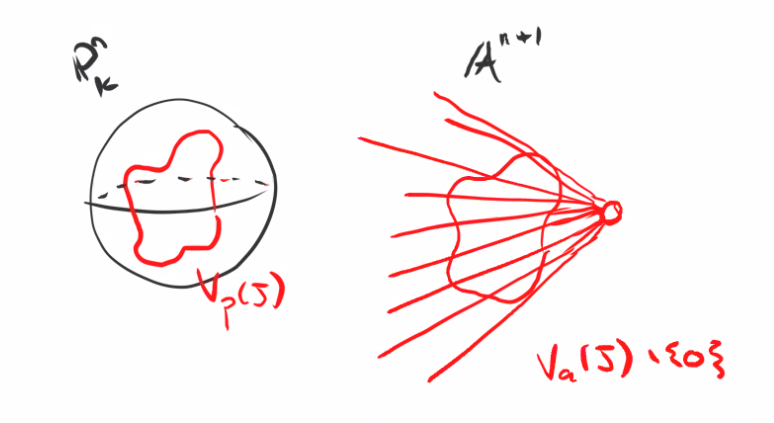
\includegraphics{figures/image_2020-11-05-10-10-38.png}
\caption{Image}
\end{figure}

By the affine Nullstellensatz,
\begin{align*}  
V_a(J) = \ts{0} \iff \sqrt{J} = I_0
.\end{align*}

Thus
\(I_p(V_p(J)) = \gens{f \st \text{homogeneous vanishing on }V_a(J)}\).
Using the fact that \(V_a(J)\) is a cone, its ideal is homogeneous and
thus generated by homogeneous polynomials by part (b) of the previous
proposition. Thus
\begin{align*}  
I_p(V_p(J)) = I_a(V_a(J)) = \sqrt J
,\end{align*} where the last equality follows from the affine
Nullstellensatz.

\end{proof}

\begin{corollary}[?]

There is an order-reversing bijection
\begin{align*}  
\correspond{\text{Projective varieties} \\ X\subset \PP^n}
&\iff
\correspond{\text{Homog non-irrelevant radical ideals} \\ \in \kx{n}} \\
X &\mapsto I_p(X) \\
? &\mapsfrom ?
.\end{align*}

\end{corollary}

\begin{remark}

A better definition of a cone over \(X\subset \PP^n_{/k}\) is
\(\bar{\pi^{-1}(X)} \subset \AA^{n+1}_{/k}\) where
\begin{align*}  
\pi: \AA^{n+1}\smz &\to \PP^n \\
\tv{x_0, \cdots, x_n} &\mapsto \tv{x_0: \cdots: x_n}
.\end{align*}

\end{remark}

\begin{definition}[Projective coordinate ring]

Given \(X\subset \PP^n\) a projective variety, the \textbf{projective
coordinate ring} of \(X\) is given by
\begin{align*}  
S(X) \da \kx{n} / I_p(X)
.\end{align*}

\end{definition}

\begin{remark}

This is a graded ring since \(I_p(X)\) is homogeneous. This follows
since the quotient of a graded ring by a homogeneous ideal yields a
grading on the quotient.

\end{remark}

\begin{remark}

We have relative versions of everything. Projective subvarieties of
projective varieties are given by \(Y\subset X\subset \PP^n\) where
\(X\) is a projective variety. We have a topology on \(X\) where the
closed subsets are projective subvarieties.

\end{remark}

\begin{remark}

Given \(J\subset S(X)\), where \(S(X)\) is the projective coordinate
ring of \(X\) and has a grading, we can take \(V_p(J) \subset X\).
Conversely, given a set \(Y\subset S(X)\), we can take
\(I_p(Y) \subset S(X)\) those homogeneous elements vanishing on \(Y\).
Thus there is an order-reversing bijection
\begin{align*}  
\correspond{\text{Projective subvarieties } \\ Y\subset X}
\iff
\correspond{\text{Homogeneous nonirrelevant radical ideals} \\ I \subset S(X)}
\end{align*} and \(S(X) = \kx{n}/J \subset \bar{I_0}\).

\end{remark}

\begin{remark}

Every nontrivial homogeneous ideal \(J\) contained in \(I_0\). Why?
Suppose \(f\in J\sm I_0\) and \(f_0\neq 0\). Then \(f_0\in J\) but
\(f_0\in k\subset \kx{n}\), implying that \(1\in J\) and thus
\(J = \gens{1}\).

\end{remark}

\begin{remark}

It is sometimes useful to know that a projective variety is cut out by
homogeneous polynomials all of \emph{equal} degree, so
\(X = V (f_1, \cdots, f_m)\) with each \(f_i\) homogeneous of degree
\(d_i\). Then there is some maximum degree \(d\). We can write
\begin{align*}  
V(f_1) = V(x_0^k f_1, \cdots, x_n^k f_1 ) \qquad \forall k\geq 0 \\
X = \Intersect V(f_1) \union V(x_i)
.\end{align*} This follows because \(V\) of a product is a union of the
vanishing loci, but \(\Intersect V(x_i) = \emptyset\). The equality
follows because for all points \(\tv{x_0, \cdots, x_n} \in \PP^n\), some
\(x_i\) is nonzero.

\end{remark}

\hypertarget{tuesday-november-10}{%
\section{Tuesday, November 10}\label{tuesday-november-10}}

\hypertarget{homogenization-and-dehomogenization}{%
\subsection{Homogenization and
Dehomogenization}\label{homogenization-and-dehomogenization}}

Last time: projective varieties \(V(f_i) \subset \PP^n_{/k}\) with
\(f_i\) homogeneous. We proved the projective nullstellensatz: for any
projective variety \(X\), we have \(V_p(I_p(X))\) and for any
homogeneous ideal \(I\) with \(\sqrt{I} \neq I_0\) the irrelevant ideal,
\(I_p(V_p(I)) = \sqrt{I}\). Recall that
\(I_0 = \gens{x_0, \cdots, x_n}\). We had a notion of a projective
coordinate ring, \(S(X) \da \kx{n} / I_p(X)\), which is a graded ring
since \(I_p(X)\) is a homogeneous ideal.

\begin{remark}

Note that \(S(X)\) is not a ring of functions on \(X\): e.g.~for
\(X= \PP^n\), \(S(X) = \kx{n}\) but \(x_0\) is not a function on
\(\PP^n\). This is because
\(f\qty{\tv{x_0: \cdots : x_n}} = f\qty{\tv{\lambda x_0: \cdots : \lambda x_n}}\)
but \(x_0\neq \lambda x_0\). It still makes sense to ask if \(f\) is
zero, so \(V_p(f)\) is a well-defined object.

\end{remark}

\begin{definition}[Dehomogenization of functions and ideals]

Let \(f\in \kx{n}\) be a homogeneous polynomial, then we define its
dehomogenization as
\begin{align*}  
f^i \da f(1, x_1, \cdots, x_n) \in k[x_1,\cdots, x_n]
.\end{align*}

For a homogeneous ideal, we define
\begin{align*}  
J^i \da \ts{f^i \st f\in J}
.\end{align*}

\end{definition}

\begin{example}

This is usually not homogeneous. Take
\begin{align*}  
f &= x_0^3 + x_0 x_1^2 + x_0 x_1 x_2 + x_0^2 + x_1 \\
\implies f^i &= 1  +x_1^2 + x_1 x_2 + x_1
,\end{align*} where has terms of mixed degrees.

\end{example}

\begin{remark}

\envlist

\begin{itemize}
\tightlist
\item
  \((fg)^i = f^i g^i\),
\item
  \((f+g)^i = f^i + g^i\)
\end{itemize}

In other words, evaluating at \(x_0 = 1\) is a ring morphism.

\end{remark}

\begin{definition}[Homogenization of a function]

Let \(f\in \kx{n}\), then the \textbf{homogenization} of \(f\) is
defined by
\begin{align*}  
f^h \da x_0^d f\qty{ {x_1 \over x_0}, \cdots, {x_n \over x_0} }
\end{align*} where \(d\da \deg(f)\).

\end{definition}

\begin{example}[?]

Let \(f(x_1, x_2) = 1 + x_1^2 + x_1 x_2 + x_2^3\), then
\begin{align*}  
f^h(x_0, x_1, x_2) = x_0^3 + x_0 x_1^2 + x_0 x_1 x_2 + x_2^3
,\end{align*} which is a homogeneous polynomial of degree \(3\). Note
that \((f^h)^i = f\).

\end{example}

\begin{example}[?]

It need not be the case that \((f^i)^h = f\). Take
\(f = x_0^3 + x_0 x_1 x_2\), then \(f^i = 1 + x_1 x_2\) and
\((f^i)^h = x_0^2 + x_1 x_2\). Note that the total degree dropped, since
everything was divisible by \(x_0\).

\end{example}

\begin{remark}

\begin{align*}  
(f^i)^h = f \iff x_0 \notdivides f
.\end{align*}

\end{remark}

\begin{definition}[Homogenization of an ideal]

Given \(J\subset \kx{n}\), define its \textbf{homogenization} as
\begin{align*}  
J^h \da \ts{f^h \st f\in J}
.\end{align*}

\end{definition}

\begin{example}

This is not a ring morphism, since \((f+g)^h \neq f^h + g^h\) in
general. Taking \(f = x_0^2 + x_1\) and \(g= -x_0^2 + x_2\), we have
\(f^h + g^h = x_0 x_1 + x_0 x_2\) while \((f+g)^h = x_12 + x_2\).

\end{example}

\begin{remark}

What is the geometric significance? Set
\begin{align*}
U_0 \da \ts{\tv{x_0: \cdots :x_n} \in \PP^n_{/k} \st x_0 \neq 0 } \cong \AA^n_{/k}
\end{align*} with coordinates
\(\tv{{x_1\over x_0} : \cdots : {x_n \over x_0}}\).

\end{remark}

\begin{proposition}[?]

The conclusion is thus that \(U_0\) with the subspace topology is equal
to \(\AA^n\) with the Zariski topology.

\end{proposition}

\begin{proof}[?]

If we define the Zariski topology on \(\PP^n\) as having closed sets
\(V_p(I)\), we would want to check that \(\AA^n\cong U_0 \subset \PP^n\)
is closed in the subspace topology. This amounts to showing that
\(V_p(I) \intersect U_0\) is closed in \(\AA^n \cong U_0\). We can check
that
\begin{align*}  
V_p(f, f\in I) = \ts{\tv{x_0:\cdots:x_n} \st f(\vector x) = 0 \, \forall f\in I}
.\end{align*} Intersecting with \(U_0\) yields
\(\ts{\tv{x_1:\cdots:x_n} \st f(\vector x) = 0,\, x_0\neq 0}\).
Equivalently, we can rewrite this set as
\begin{align*}
\ts{\tv{x_1:\cdots:x_n} \st f\qty{\tv{1, {x_1 \over x_0}, \cdots,{x_n \over x_0} }} = 0,\, f \text{ homogeneous}}
\end{align*} Since these are coordinates on \(\AA^1\), we have
\(V_p(I) \intersect U_0 = V_a(I^i)\) which is closed.

Conversely, given a closed set \(V(I)\), we can write this as
\(V(I) = U_0 \intersect V_p(I^h)\).

\end{proof}

\begin{corollary}[?]

\(\PP^n\) is irreducible of dimension \(n\), where the proof is that its
covered by irreducible topological spaces of dimension \(n\) with
nonempty intersection combined with a fact from the exercises.

\end{corollary}

\begin{example}[?]

Consider \(f(x_1, x_2) = x_1^2 - x_2^2 - 1\) and consider
\(V(f) \subset \AA^2_{/\CC}\):

\begin{figure}
\centering
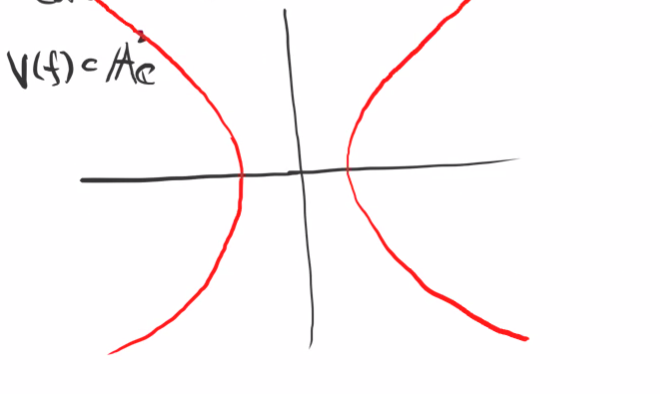
\includegraphics[width=3.64583in,height=\textheight]{figures/image_2020-11-10-10-10-42.png}
\caption{Image}
\end{figure}

Note that for real projective space, we can view this as a sphere with
antipodal points identified. We can thus visualize this in the following
way:

\begin{figure}
\centering
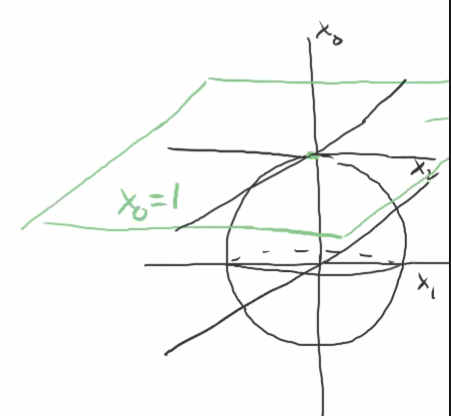
\includegraphics[width=3.64583in,height=\textheight]{figures/image_2020-11-10-10-12-20.png}
\caption{O}
\end{figure}

We can normalize the \(x_0\) coordinate to one, hence the plane. We can
also project \(V(f)\) from the plane onto the sphere, mirroring to
antipodal points:

\begin{figure}
\centering
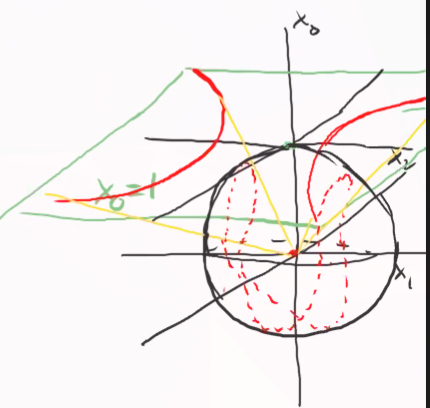
\includegraphics[width=3.64583in,height=\textheight]{figures/image_2020-11-10-10-14-09.png}
\caption{Image}
\end{figure}

This misses some points on the equator, since we aren't including points
where \(x_0 = 0\). Consider the homogenization
\(V(f^h) \subset \PP^2_{/\CC}\). It's given by
\(f^h = x_1^2 - x_2^2 - x_0^2\), then
\begin{align*}  
V(f^h) \intersect V(x_0) = \ts{\tv{0:x_1:x_2} \st f^h(0, x_1, x_2) = 0 } = \ts{\tv{0:1:1}, \tv{0:1:-1}}
,\end{align*} which can be seen in the picture as the points at
infinity:

\begin{figure}
\centering
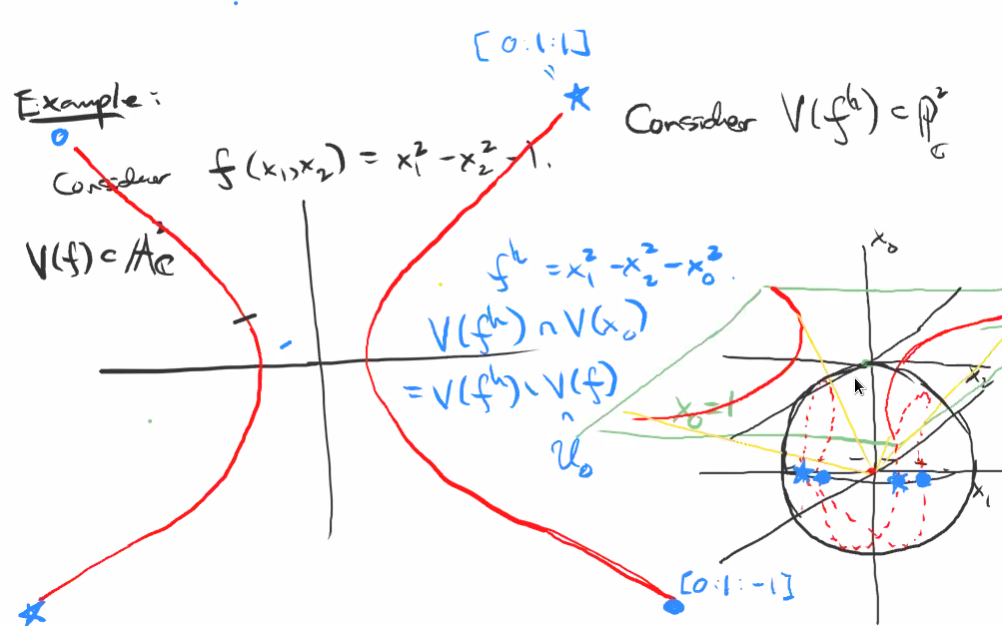
\includegraphics[width=4.6875in,height=\textheight]{figures/image_2020-11-10-10-19-19.png}
\caption{A}
\end{figure}

Note that the equator is
\(V(x_0) = \PP^2_{/\CC}\sm U_0 \cong \PP^2\sm \AA^2\). So we get a
circle of points at infinity,
i.e.~\(V(x_0) = \PP^1 = \ts{\tv{0:v_1:v_2}}\).

\end{example}

\begin{example}[?]

Consider \(V(f)\) where \(f\) is a line in \(\AA^2_{/\CC}\), say
\(f = ax_1 + bx_2 + c\). This yields \(f^h = ax_1 + bx_2 + cx_0\) and we
can consider \(V(f^h) \cong \PP^2_{\CC}\). We know \(\PP^1_{\CC}\) is
topologically a sphere and \(\AA^1_{/\CC}\) is a point:

\begin{figure}
\centering
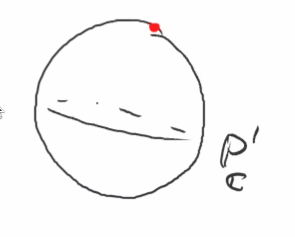
\includegraphics[width=2.60417in,height=\textheight]{figures/image_2020-11-10-10-26-40.png}
\caption{\(\PP^1_{\CC}\)}
\end{figure}

The points at infinity correspond to
\begin{align*}  
V(f^h) = V(f^h) \intersect V(x_0) = \ts{\tv{0:-b:a}}
,\end{align*} which is a single point not depending on \(c\).

\end{example}

\begin{remark}

\(\PP^2_{/k}\) for any field \(k\) is a \textbf{projective plane}, which
satisfies certain axioms:

\begin{enumerate}
\def\labelenumi{\arabic{enumi}.}
\item
  There exists a unique line through any two distinct points,
\item
  Any two distinct lines intersect at a single point.
\end{enumerate}

A famous example is the \emph{Fano plane}:

\begin{figure}
\centering
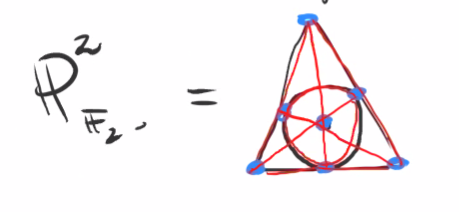
\includegraphics{figures/image_2020-11-10-10-29-34.png}
\caption{Fano Plane}
\end{figure}

Why is this true? \(\PP^2_{/k}\) is the set of lines in \(k^3\), and the
lines in \(\PP^2_{/k}\) are the vanishing loci of homogeneous
polynomials and also planes in \(k^3\), since any two lines determine a
unique plane and any two planes intersect at the origin.

\end{remark}

\begin{proposition}[?]

Let \(J\subset \kx{n}\) be an ideal. Let \(X \da V_a(J) \subset \AA^n\)
where we identify \(\AA^n = U_0 \subset \PP^n\). Then the closure
\(\bar{X} \subset \PP^n\) is given by \(\bar{X} = V_p(J^h)\). In
particular, \(V_a(J) = V_p(J^h)\).

\end{proposition}

\begin{proof}[?]

Note that it's clear that \(V_p(J^h)\) is closed and contains
\(V_a(J)\). For the reverse containment, let \(Y\containing X\) be
closed; we want to show that \(Y\contains V_p(J^h)\). Since \(Y\) is
closed, \(Y = V_p(J')\) where \(J'\) is some homogeneous ideal. Any
element \(f'\in J'\) satisfies \(f' = x^d f\) for some maximal \(d\)
where \(x_0^d f\) vanishes on \(X\). We also have \(f=0\) on \(X\) since
\(X\subset U_0\). We can compute
\begin{align*}  
f\in I_a(X) = I_a(V_a(J)) = \sqrt J
,\end{align*} so \(f^m\in J\). Then \((f^h)^m \in J^h\) for some \(m\),
and this \(f^h \in \sqrt{J^h}\).

We can conclude that \(J'\subset \sqrt J\), which shows that
\(V_p(J') \contains V_p(J^h)\) as desired.

\end{proof}

\begin{definition}[Projective Closure]

The \textbf{projective closure} of \(X = V_a(J)\) is the smallest closed
subset containing \(X\) and is given by
\begin{align*}  
\bar{X} = V_p(J^h)
.\end{align*}

\end{definition}

\hypertarget{thursday-november-12}{%
\section{Thursday, November 12}\label{thursday-november-12}}

Recall that if \(f\in \kx{n}\) is a homogeneous degree \(d\) polynomial,
then \(f^i \da f(1, x_1, \cdots, x_n) \in k[x_1,\cdots, x_n]\) is the
dehomogenization of \(f\). Conversely,
\(f^h \da x_0^d f\qty{ {x_1 \over x_0}, \cdots, {x_n \over x_0} }\) is
the homogenization. This is related to looking at the open subset
\(U_0 \da {\ts x\in \PP^n_{/k} \st x_0\neq 0} \subseteq \PP^n_{/k}\),
where we found that \(U_0 \cong \AA^n_{/k}\).

\begin{proposition}[Projective Closure]

Let \(V(I) \subset U_0\) be an affine variety, then
\(V(I) \subset \PP^n_{/k}\) is given by
\begin{align*}
V(I^h) \da \ts{f^h \st f\in I}
,\end{align*} the \textbf{projective closure}.

\end{proposition}

\begin{remark}

Projective varieties are better! They're closed in the classical
topology, and subsets of projective space and thus compact.

\end{remark}

\begin{remark}

It doesn't suffice to just homogenize the individual generators of the
ideal \(I\). For example, take \(J \da \gens{x_1, x_2 - x_1^2}\). We
have \(V(J) \subset \AA^2\) given by \(\ts{(0, 0)}\), and by the
proposition, \(V(J^h) = \ts{[1:0:0]}\) since the single point at the
origin is closed in \(\PP^2\).

On the other hand,
\begin{align*}  
V_p(x_1, x_0 x_2 - x_1^2) = \ts{[1:0:0], [0:0:1]} \subset \PP^2
.\end{align*}

Note that \(x_2 \in J\), so this needs to be homogenized too.\footnote{It
  is possible to get around this issue computationally by using Gröbner
  bases, a special type of generating set for ideals.}

\end{remark}

\begin{remark}

An aside: how do you implement algebraic geometry? For example, when is
\(\gens{f_i} = \gens{1}\)? This is generally a somewhat difficult
problem, since checking that their corresponding varieties are equal
isn't so tractable.

\end{remark}

\hypertarget{chapter}{%
\subsection{Chapter ?}\label{chapter}}

Goal: understand and define the sheaf of regular functions on projective
varieties. Given an open subset \(U\subset V_p(J)\), what are the
regular functions on it?

\begin{definition}[?]

Let \(U\subset X\) be an open subset of a projective variety, and define
\begin{align*}  
\OO_X(U) \da \ts{\phi:U\to k \st \phi \text{ is locally of the form }   {g_p \over f_p} \in S(X)_d }
.\end{align*} i.e.~the functions in the homogeneous coordinate ring of
the same degree \(d\).

\end{definition}

\begin{remark}

Note that \(g_p/f_p\) is well-defined on \(V(f_p)^c\) since
\begin{align*}  
{ g_p(\lambda \vector x) \over  f_p(\lambda \vector x)} 
= { \lambda^d g_p(\vector x) \over \lambda^d f_p(\vector x) }
= {g_p(\vector x) \over f_p (\vector x)}
\end{align*}

\end{remark}

Recall that ``locally of the form \(\cdots\)'' means that for all
\(p\in U\), there exists an open neighborhood \(U_p\) on which
\(\ro{\phi}{U_p} = g_p / f_p\).

\begin{definition}[Projective Variety as a Ringed Space]

Note that if \(X\subset \PP^n\) is closed, then \(X\intersect U_i\) is
closed and thus an affine variety.
\begin{align*}  
\tilde \OO_X(U) \da \ts{\phi: U\to k \st \ro{\phi}{U\intersect U_i} \text{ is a regular function} }
.\end{align*}

\end{definition}

\begin{proposition}[?]

These two definitions are equivalent.

\end{proposition}

\begin{proof}[?]

It suffices to check that
\(\OO_{X\intersect U_i} = \tilde \OO_{X\intersect U_i}\) as sheaves on
\(X\intersect U_i\), i.e.~checking on an open cover, since then they'd
both arise from the gluing construction. We have
\begin{align*}  
X\intersect U_i = \ts{[x_0 : \cdots: x_n] \st x_i \neq 0 }
.\end{align*}

Let \(V\subset X\intersect U_0\) be an open subset, we then want to show
that \(\OO_X(V)\) are the regular functions on \(V\) when \(V\) as a
subset of an affine variety. So let \(\phi\in \OO_X(V)\), so that
locally \(\phi = g_p/f_p \in S(X)_d\) as a ratio of two homogeneous
polynomials. We want to know if \(\phi\) can be written as the ratio of
two polynomials in one additional variable, so we just dehomogenize to
obtain \(\phi = g^i_p / f^i_p\) locally where both are in
\(A(X\intersect U_0)\). So \(\phi\) is a regular function on the open
subset \(V\) of the affine variety \(X\intersect U_0\).\\

Conversely, suppose that \(\phi = g_p/f_p \in A(X\intersect X_0)\)
locally around \(p\). It's not necessarily the case that
\(\phi = g^h_p / f^h_p\), but it is true that
\begin{align*}  
\phi = {x_0^d g_p^h \over f_p^h} = {g_p^h \over x_0^{-d} f_p^h}
,\end{align*} where \(d = \deg f^h - \deg g^h\). This is locally a ratio
of two homogeneous polynomials of equal degree, so \(\OO_X\) and
\(\tilde \OO_X\) define the same sheaf of functions on \(X\).

\end{proof}

\hypertarget{morphisms-of-projective-varieties}{%
\subsection{Morphisms of Projective
Varieties}\label{morphisms-of-projective-varieties}}

\begin{lemma}[?]

Let \(X\) be a projective variety and \(f_0, \cdots, f_m \in S(X)_d\).
Then on the open subset \(X\sm V(f_i)\), there is a morphism
\begin{align*}  
f: U &\to \PP^m \\
p &\mapsto \tv{f_0(p) : \cdots : f_m(p) }
.\end{align*}

\end{lemma}

\begin{proof}[?]

This map is well-defined, since letting \(p = [x_0: \cdots : x_n]\) we
have
\begin{align*}  
[\lambda x_0 : \cdots : \lambda x_n] 
&\mapsto 
[ \lambda^d f_0(p) : \cdots : \lambda^d f_m(p)] 
= f(p)
.\end{align*}

We need to check that

\begin{enumerate}
\def\labelenumi{\arabic{enumi}.}
\item
  \(f\) is continuous, and
\item
  The pullback of a regular function on any open set is again regular.
\end{enumerate}

\begin{claim}

\(f\) is continuous.

\end{claim}

Consider \(f^{-1}(V(h))\) with \(h\in k[y_0, \cdots, y_m]\) homogeneous.
We can check that
\begin{align*}  
f^{-1}(V_p(h)) = V_p(h(f_0, \cdots, f_m))
,\end{align*} which is closed, so \(f\) is continuous.

\begin{claim}

\(f\) pulls back regular functions.

\end{claim}

Let \(h_1, h_2 \in S(\PP^m)\) be homogeneous polynomials of equal degree
in \(k[y_0, \cdots, y_m]\). Then on \(V(h_2)^c\), we have
\begin{align*}  
f^*\qty{h_1 \over h_2 } = {h_1(f_0, \cdots, f_m) \over h_2(f_0, \cdots, f_m)}
.\end{align*} This is a ratio of homogeneous polynomials of equal degree
in the \(x_i\), the pullback is again locally homogeneous ratios of
functions of equal degree.

\end{proof}

\hypertarget{tuesday-november-17}{%
\section{Tuesday, November 17}\label{tuesday-november-17}}

\hypertarget{projecting-from-a-point}{%
\subsection{Projecting From a Point}\label{projecting-from-a-point}}

We have \(\PP^n \da \AA^{n+1}\smz / \sim\) where \(x\sim \lambda x\),
and projective varieties \(V(I) \subset \PP^n\) where
\(I \normal k[x_0, \cdots, x_n]\) is a homogeneous ideal. We defined a
sheaf of rings \(\OO_X\) on \(X = V(I)\) by
\begin{align*}  
\OO_X(U) \da \ts{\phi: U\to k \st \phi \text{ is locally a ratio of two homogeneous polynomials of equal degree}}
.\end{align*} We showed that this was the same as the sheaf
\(\tilde \OO_X\) defined by gluing ringed spaced
\((X \intersect U_i, \OO_{X\intersect U_i})\) where \(U_i = D(x_i)\). We
also showed that \(S(X) \da k[x_0, \cdots, x_n] / I(X)\) is homogeneous,
i.e.~the quotient by a homogeneous ideal is again homogeneous. Moreover,
if \(\ts{f_i}_{i=0}^m \subseteq S(X)_d\) and
\(V(\ts{f_i}) = \emptyset\). then the map
\begin{align*}  
(f_0, \cdots, f_m): X &\to \PP^m \\
x &\mapsto [f_0(x), \cdots, f_m(x)]
.\end{align*}

Recall that a variety is separated iff \(\Delta \injects X\) is closed.
Let \(A\in \GL_{n+1}(k)\) and define a map
\begin{align*}  
A: \PP^n &\to \PP^n \\
\begin{bmatrix}
x_0  \\
\vdots \\
x_n 
\end{bmatrix}
&\mapsto
A
\begin{bmatrix}
x_0  \\
\vdots \\
x_n 
\end{bmatrix}
.\end{align*}

This is a morphism because
\begin{align*}  
\begin{bmatrix}
- & \vec A_0 & - \\
- & \vdots & - \\
- & \vec A_n & - \\
\end{bmatrix}
\begin{bmatrix}
x_0  \\
\vdots \\
x_n 
\end{bmatrix}
=
\begin{bmatrix}
A_0 \cdot \vector x  \\
\vdots \\
A_n \cdots \vector x 
\end{bmatrix}
,\end{align*} which are linear homogeneous polynomials.

Then \(V_p(A_i \cdot \vector x) = \emptyset\), and thus
\(V_a(A_i \cdot \vector A) = \ts{0}\). So we should view
\(A\in \PGL_{n+1}(k)\). Note that this is a group, since \(A^{-1}\)
again forms a morphism. Thus \(\PGL_{n+1}(k) \subset \Aut(\PP^n)\), and
it turns out that these are in fact equal.

\begin{definition}[Projection from a point]

Let \(a = [1: 0 : \cdots : 0] \in \PP^n\), then there is a morphism
\begin{align*}  
\PP^n \sm\ts{a} &\to \PP^{n-1} \\
[x_0: \cdots : x_n] &\mapsto [x_1: \cdots : x_n]
.\end{align*} Note that this morphism does not extend to \(\PP^n\).

More generally, given any point \(p\in \PP^n\), we can project from it
by making a linear change of coordinates to \(p = [1: 0 : \cdots : 0]\).

\end{definition}

Let \(x\in \PP^n\sm\ts{a}\), then there is a unique line through \(a\)
and \(x\). It can be described parametrically as follows: writing
\(x = [x_0: \cdots : x_n]\), we take the plane they span and
projectivize to obtain \(s[x_0 : \cdots : x_n] + t [1: 0 : \cdots : 0]\)
where we range over \([s: t] \in \PP^1\). In fact, this defines a
morphism \(\PP^1 \to \PP^n\).

Consider now \(\PP^{n-1} = V(x_0)\), this copy of \(\PP^{n-1}\)
intersects any such line at a unique point:

\begin{figure}
\centering
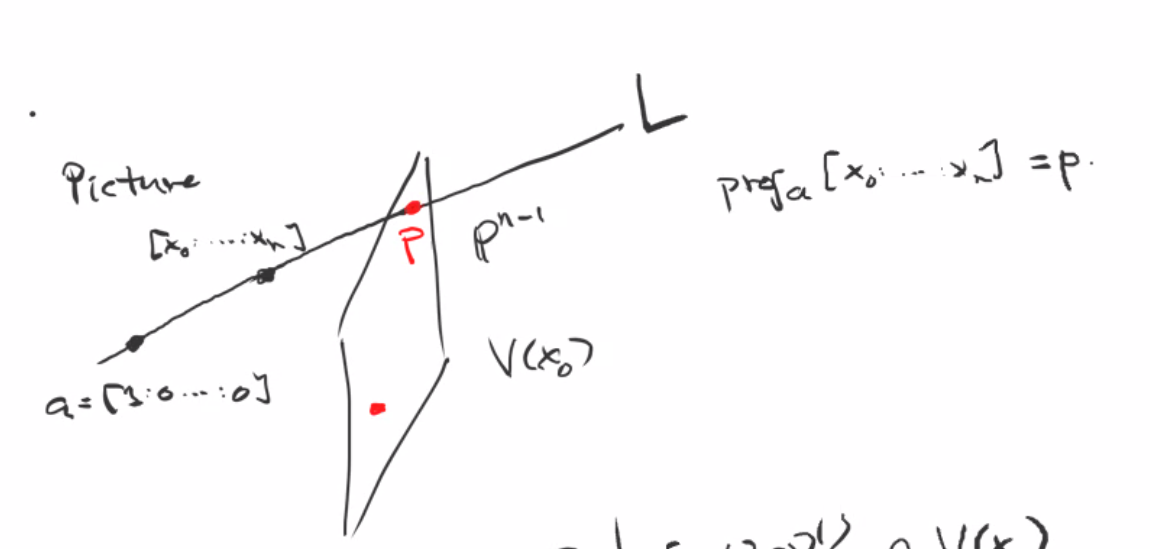
\includegraphics{figures/image_2020-11-17-10-10-32.png}
\caption{Image}
\end{figure}

\begin{example}[?]

Consider \(X = V(x_0 x_2 - x_1^2) \subset \PP^2\), which defines a
conic, and the projection \(\PP^2 \sm \ts{[1:0:0]} \to \PP^1\):

\begin{figure}
\centering
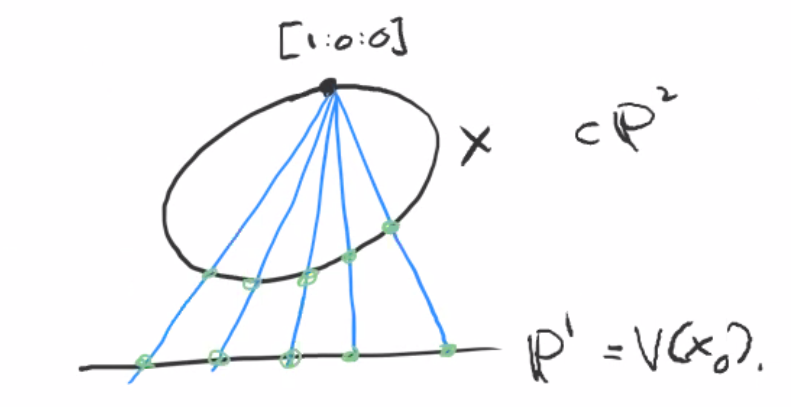
\includegraphics{figures/image_2020-11-17-10-13-40.png}
\caption{Projection onto \(V(x_0)\).}
\end{figure}

This morphism can be restricted to \(\phi: X\sm\ts{[1:0:0]} \to \PP^2\),
and the claim is that this morphism extends to all of \(X\). The secant
lines approach a tangent line at \([1:0:0]\), which \(V(x_0)\) at a
unique point. So we define
\begin{align*}  
\bar \phi \da 
\begin{cases}
[x_1: x_2] & x \neq [1:0:0] \\
[x_0: x_1] & \neq [0:0:1]
\end{cases}
.\end{align*}

This locally writes \(\phi\) as a morphism, so we only need to check
that they agree on the overlap. Note that on \(X\), we have
\([x_1: x_2] = [x_0 : x_1]\) wherever both are well-defined. In fact,
\(\bar \phi\) is an isomorphism, since an inverse can be explicitly
written. Thus \(X\cong \PP^1\), and in fact all nondegenerate conics are
isomorphic to \(\PP^1\) as well. Here nondegenerate means that if \(Q\)
is a quadratic polynomials in \(x_0, x_1, x_2\), then \(Q\) does not
factor as a product of linear factors. Note that such a \(Q\) is a
quadratic form, so \(Q(x) = B(x, x)\) for some bilinear form, and \(Q\)
is nondegenerate if \(\det B \neq 0\) where \(B_{ij} = B(e_i, e_j)\).

\end{example}

\hypertarget{the-segre-embedding}{%
\subsection{The Segre Embedding}\label{the-segre-embedding}}

\begin{definition}[?]

Letting \(N = (n+1)(m+1) - 1\), the \textbf{Segre embedding} is the
morphism
\begin{align*}  
f: \PP^n \cross \PP^m &\to \PP^N \\
([x_0: \cdots : x_n], [y_0: \cdots : y_m]) &\mapsto
[x_0 y_0 : \cdots : z_{ij} = x_i y_j : x_n y_m]
.\end{align*} Note that \(\PP^n, \PP^m\) are prevarieties and we thus
know how to construct their product prevariety.

\end{definition}

Check that this is well-defined!

\begin{proposition}[Properties of the Segre embedding]

\envlist

\begin{enumerate}
\def\labelenumi{\alph{enumi}.}
\item
  The image \(X\) is a projective variety.
\item
  \(f: \PP^n \cross \PP^m \to X\) is a morphism.
\end{enumerate}

\end{proposition}

\begin{proof}[of (a)]

It suffices to write polynomials in the coordinate \(z_{ij}\) that cut
out \(f(\PP^n \cross \PP^m)\). Given \(z_{ij} = x_i y_j\), we have
\(z_{ij} z_{kl} = z_{il} z_{kj}\) and
\((x_i y_j)(x_k y_l) = (x_i y_l)(x_k y_j)\). The former quadric
equations in \(z_{ij}\) variables vanish on \(f(\PP^n \cross \PP^m)\).
The claim is that \(V(z_{ij} z_{kl} - z_{il} z_{kj})\) works.

Note that wlog, we can assume \(z_{00} = 1\), in which case
\(z_{ij} z_{00} = z_{ij} = z_{i0} z_{0j}\) on \(X\). Setting
\(x_i = z_{i0}\) and \(y_j = z_{0j}\), we've now constructed a point in
the preimage, so \(f\) surjects onto \(X\).

\end{proof}

\begin{proof}[of (b)]

That \(f\) is a morphism to \(\PP^n\) is easy, and since
\(\im f \subset X\), \(f: \PP^n \cross \PP^m \to X\) is a morphism. On
\(D(z_{00}) \subset X\), the inverse described above is a morphism.
Since this works for any \(z_{ij}\), \(f^{-1}\) is well-defined and a
morphism, making \(f\) an isomorphism.

\end{proof}

\begin{example}[?]

\begin{figure}
\centering
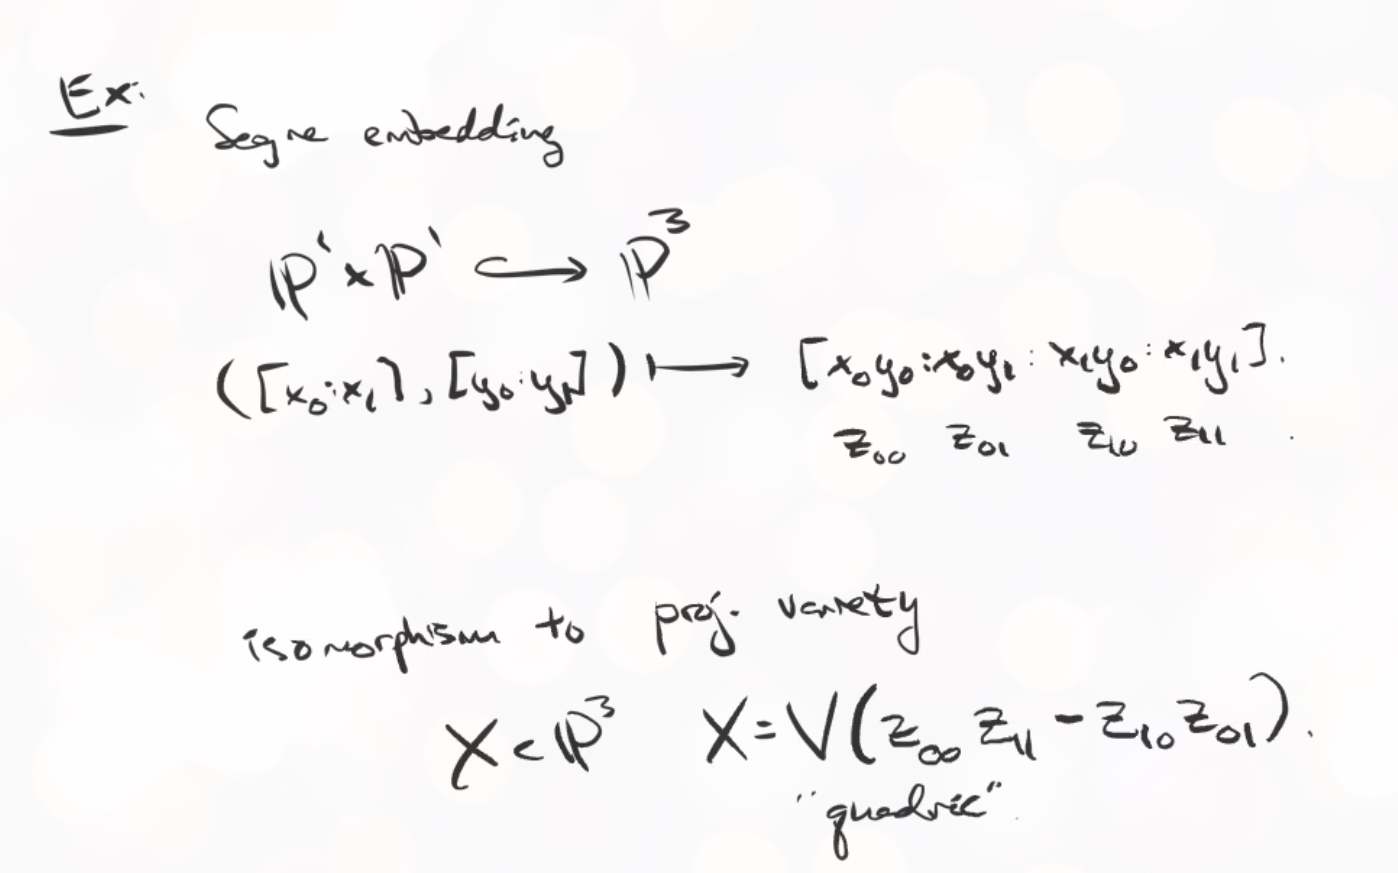
\includegraphics{figures/image_2020-11-17-10-42-49.png}
\caption{Image}
\end{figure}

\end{example}

\hypertarget{thursday-november-19}{%
\section{Thursday, November 19}\label{thursday-november-19}}

\hypertarget{why-use-projective-varieties}{%
\subsection{Why use projective
varieties?}\label{why-use-projective-varieties}}

For e.g.~a manifold, there is a well-defined intersection pairing, and
the same way that \([\mu] \in H^1(T, \ZZ) = 1\) in the torus, we have
\([L]^2 = 1\) in \(\PP^2_{/\CC}\), so every two lines intersect in a
unique point. Also, Bezout's theorem: any two curves of degrees \(d, e\)
in projective space intersect in \(d\cdot e\) points. Also note that we
have a notion of compactness that works in the projective setting but
not for affine varieties.

\hypertarget{projective-varieties-are-varieties}{%
\subsection{Projective Varieties are
Varieties}\label{projective-varieties-are-varieties}}

Last time: we saw the Segre embedding
\((\vector x, \vector y)\mapsto [x_i y_j]\), which was an isomorphism
onto its image \(X = V(z_{ij}z_{kl} - z_{ik} z_{kj} )\), which exhibits
\(\PP^n \cross \PP^m\) as a projective variety.

\begin{example}[?]

For \(\PP^1 \cross \PP^1 \to \PP^3\), its image is \(X = V_p(xy - zw)\),
which is a quadric (vanishing locus of a degree 4 polynomial).

\begin{figure}
\centering
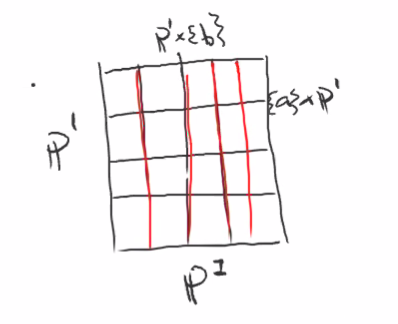
\includegraphics{figures/image_2020-11-19-09-45-47.png}
\caption{Image}
\end{figure}

The projection map has fibers, which induce a \emph{ruling} (a family of
\(\PP^1\)s), which we can see from the real points:

\begin{figure}
\centering
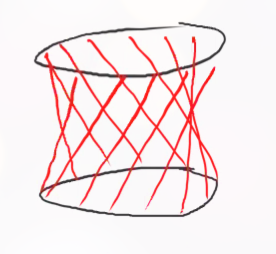
\includegraphics{figures/image_2020-11-19-09-46-38.png}
\caption{Image}
\end{figure}

\end{example}

\begin{corollary}[?]

Every projective variety is a separated prevariety, and thus a variety.

\end{corollary}

\begin{proof}[?]

It suffices to show that \(\Delta_X \subset X\cross X\) is closed. We
can write
\begin{align*}  
\Delta_{\PP^n} = 
\ts{
[x_0: \cdots: x_n], [y_0: \cdots : y_n] \st
x_i y_j - x_j y_i = 0 \, \forall i, j
}
.\end{align*} This says that \(\vector x, \vector y\) differ by scaling.
We know that \(\Delta_{\PP^n} \injects \PP^n \cross \PP^n\), which is
isomorphic to the Segre variety \(S_V\) in \(\PP^{(n+1)^2 -1}\), and we
can write \(z_{ij} = x_i y_j\) and thus
\begin{align*}  
\Delta_{\PP^n} = S_V \intersect V(z_{ij} - z_{ji})
.\end{align*} Note that the Segre variety is closed.

The conclusion is that \(\PP^n\) is a variety, and any closed
subprevariety of a variety is also a variety by taking
\(\Delta_{\PP^n} \intersect (X\cross X) = \Delta_X\), which is closed as
the intersection of two closed subsets.

\end{proof}

\begin{definition}[Closed Maps]

Recall that a map \(f:X\to Y\) is topological spaces is \textbf{closed}
if whenever \(U \subset X\) is closed, then \(f(U)\) is closed in \(Y\).

\end{definition}

\begin{definition}[Complete Varieties]

A variety \(X\) is \textbf{complete} if the projection
\(\pi_Y: X\cross Y \surjects Y\) is a closed map for any \(Y\).

\begin{quote}
Slogan: analog of compactness.
\end{quote}

\end{definition}

\begin{proposition}[?]

The projection \(\PP^n \cross \PP^m \to \PP^m\) is closed.

\end{proposition}

\begin{proof}[?]

Let \(Z \subset \PP^n \cross \PP^m\), and write \(Z = V(f_i)\) with
\(f_i \in S(S_V)\). Note that if the \(f_i\) are homogeneous of degree
\(d\) in \(z_{ij}\), the pulling back only the isomorphism
\(\PP^n\cross \PP^m \to S_V\) yields \(z_{ij} = x_i y_j\) and
polynomials \(h_i\) which are homogeneous polynomials in \(x_i, y_j\)
which have degree \(d\) in both the \(x\) and \(y\) variables
individually. Consider \(a\in \PP^m\), we want to determine if
\(a\in \pi(Z)\) and show that this is a closed condition. Note that
\(a\not\in \pi(Z)\)

\begin{itemize}
\item
  \(\iff\) there does not exists an \(x\in \PP^n\) such that
  \((x, a) \in Z\)
\item
  \(\iff\) \(V_p(f_i(x, a))_{i=1}^r = \emptyset\)
\item
  \(\iff\) \(\sqrt{\gens{f_i(x, a)}_{i=1}^r } = \gens{1}\) or the
  irrelevant ideal \(I_0\)
\item
  \(\iff\) there exist \(k_i \in \NN\) such that
  \(x_i^{k_i} \in \gens{f_i(x, a)}_{i=1}^r\)
\item
  \(\iff\) \(\kx{n}_k \subset \gens{f_i(x, a)}_{i=1}^r\) (where this is
  the degree \(k\) part)
\item
  \(\iff\) the map
  \begin{align*}  
  \Phi_a: \kx{n}_{d - \deg f_2} \oplus \cdots \oplus \kx{n}_{d - \deg f_r} &\to \kx{n}_d \\
  (g_1, \cdots, g_r) &\mapsto \sum f_i(x, a) g_i (x, a)
  \end{align*} is surjective.
\end{itemize}

Recap: we have a closed subset of \(\PP^n \cross \PP^m\), want to know
its projection is closed. We looked at points not in the closed set,
this happens iff the degree \(d\) part of the polynomial is not
contained in the part where we evaluate by \(a\). This reduces to a
linear algebra condition: taking arbitrary linear combinations yields a
surjective map. Thus \(a\in \pi(Z)\) iff \(\Phi_a\) is \emph{not}
surjective.\\

Expanding in a basis, we can write \(\Phi_a\) as a matrix whose entries
are homogeneous polynomials in the coordinates of \(a\). Moreover,
\(\Phi_a\) is not surjective iff all \(d\times d\) determinants of
\(\Phi_a\) are nonzero (since this may not be square). This is a
polynomial condition, so \(a\in \pi(Z)\) iff a bunch of homogeneous
polynomials vanish, making \(\pi(Z)\) is closed.

\end{proof}

\begin{corollary}[?]

The projection \(\pi: \PP^n\cross Y\to Y\) is closed for any variety
\(Y\), making \(\PP^n\) complete.

\end{corollary}

\begin{proof}[?]

How to prove anything for varieties: use the fact that they're glued
from affine varieties, so prove in that special case. So first suppose
\(Y\) is affine. Let \(Z \subset \PP^n \cross Y\) be closed, and
consider \(\bar Y ss \PP^m\) and
\(\bar Z \subset\PP^n \cross \bar Y \subset\PP^n \cross \PP^m\) as a
closed subset. Then we know that the projection
\(\pi: \PP^n \cross \PP^m \to \PP^m\) is closed, so
\(\pi(\bar Z) \subset\PP^m\) is closed. But we can write
\(\pi(Z) = \pi(\bar Z \intersect \PP^n \cross Y) = \pi(\bar Z) \intersect Y\)
which is closed. So \(\pi(Z)\) is closed in \(Y\), which proves this for
affine varieties.\\

Supposing now that \(Y\) is instead glued from affines, it suffices to
check that the set is closed in an open cover. So \(Z \subset X\) is
closed if when we let \(X = \union U_i\), we can show
\(Z \intersect U_i\) is closed. But this essentially follows from above.

\end{proof}

\begin{corollary}[?]

Any projective variety is complete.

\end{corollary}

\begin{proof}[?]

If \(X \subset \PP^n\) is closed and if \(\PP^n \cross Y\to Y\) is a
closed map for all \(Y\), then restricting to \(X\cross Y\to Y\) again
yields a closed map.

\end{proof}

\begin{corollary}[?]

Let \(f:X\to Y\) be a morphism of (importantly) \emph{varieties} and
suppose \(X\) is complete. Then \(f(X)\) is closed in \(Y\).

\end{corollary}

\begin{proof}[?]

Consider the graph of \(f\),
\(\Gamma_f = \ts{(x, f(x))} \subset X\cross Y\). From a previous proof,
we know \(\Gamma_f\) is closed when \(Y\) is a variety (by pulling back
a diagonal). So \(\Gamma_f\) is closed in \(X\cross Y\), and thus
\(\pi_Y(\Gamma_f) = f(X)\) is closed because \(X\) is complete.

\end{proof}

\begin{corollary}[?]

Let \(X\) be complete, then \(\OO_X(X) = k\), i.e.~every global regular
function is constant.

\end{corollary}

Note: this is an analog of the maximum modulus principle: if \(X\) is a
compact complex manifold, then any function that is holomorphic on all
of \(X\) is constant.

\begin{proof}[?]

Suppose \(\phi X\to \AA^1\) is a regular function. Since
\(\AA^1 \subset \PP^1\), extend \(\phi\) to a morphism
\(\hat \phi: X\to PP^1\). By a previous corollary, \(\phi(X)\) is
closed, but \(\infty \not\in \phi(X)\) implies \(\phi(X) \neq \PP^2\),
so \(\phi(X)\) is finite. Since \(X\) is connected, \(\phi(X)\) is a
point, making \(\phi\) a constant map.

\end{proof}

\hypertarget{tuesday-november-24}{%
\section{Tuesday, November 24}\label{tuesday-november-24}}

\hypertarget{the-veronese-embedding}{%
\subsection{The Veronese Embedding}\label{the-veronese-embedding}}

\begin{definition}[Veronese Embedding]

Let \(n, d > 0\) and let \(f_0, \cdots, f_n\) be the monomials of degree
\(d\) in \(\kx{n}\). There is a morphism
\begin{align*}  
\PP^n \sm V(f_0,\ codts, f_n) &\to \PP^N \\
\vector x &\mapsto [f_0(\vector x), \cdots, f_N(\vector x)]
,\end{align*} where \(N+1\) is the number of monomials, and is equal to
\({n+d \choose d}\).

\end{definition}

\begin{remark}

It is true that \(V(f_0, \cdots, f_N) \neq \emptyset\), since
\(V(x_0^d, x_1^d, \cdots, x_n^d) = V(x_0, \cdots, x_n)\). This will be
the Veronese embedding, although we need to prove it is an embedding. On
an open set \(D(x_0) \subset \PP^2\) one can define an inverse. Suppose
we hyave a coordinate \(z_j = x_i^{d-1} x_j\) and \(z_i = x_i^d\) on
\(\PP^N\). Then we can take the point
\begin{align*}  
\tv{ {z_1 \over z_i}, \cdots, {z_i \over z_i}, \cdots, {z_n \over z_i} }
.\end{align*} This defines an inverse on \(D(z_i)\). Since the open sets
\(D(x_i)\) cover \(\PP^N\), we have an inverse on the entire image.

\end{remark}

\begin{remark}

This embedding converts hypersurfaces of degree \(d\) into hyperplanes.
The Veronese is an isomorphism onto its image. Consider some arbitrary
degree \(d\) element of \(S(\PP^n)\). Consider
\(X \da V(\sum_{j=1}^N a_j f_j) \subset\PP^n\), where \(a_j\in k\),
which is equal to \(\phi^{-1}(V(\sum_{j=1}^N a_j w_j ))\).

\todo[inline]{Probably not right.}

We have a picture: embedding \(\PP^n\injects \PP^N\) in some curved way
sends a hypersurface to the intersection of a hyperplane with the
embedded image:

\begin{figure}
\centering
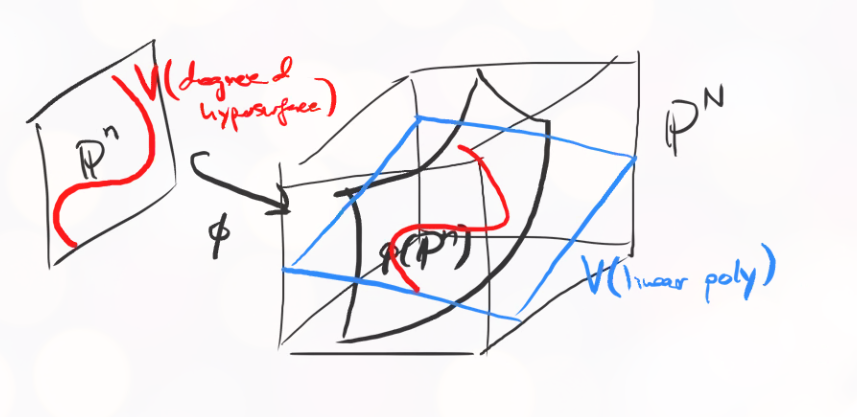
\includegraphics{figures/image_2020-11-24-09-48-27.png}
\caption{Image}
\end{figure}

\end{remark}

\begin{definition}[Hyperplane Sections]

Let \(X \subset\PP^n\) be a projective variety. A \textbf{hyperplane
section} is the intersection of \(X\) with some hyperplane
\(H \da V(f)\) for \(f\) some linear homogeneous polynomial.

\end{definition}

\begin{example}[of the Veronese embedding]

Let \(n=1\), then we get the embedding
\begin{align*}  
\PP^1 &\injects \PP^d \\
[x_0: x_1] &\mapsto [x_0^d: x_0^{d-1}x_1 : \cdots : x_0 x_1^{d-1} : x_1^d]
.\end{align*} Note that there are \(d+1\) such monomials, and not all
can simultaneously vanish. The image of this \(\PP^1\) is called the
\emph{twisted normal curve}.

\end{example}

\begin{example}[?]

Take
\begin{align*}  
\PP^1 &\injects \PP^2 \\
[x_0 : x_1] &\mapsto [x_0^2 : x_0 x_1: x_1^2]
.\end{align*} What homogeneous polynomials cut out \(\phi(\PP^1)\)?
I.e., what is \(I(\phi(\PP^1)) \subset S(\PP^2)\)? Note that
\(w_0 w_2 - w_1^2 \ro{}{\phi(\PP^1)}\), so this is an element. Is it a
generator? I.e., given any \(p\in V(w_0 w_2 - w_1^2)\) is of the form
\(p = [x_0^2 : x_0 x_1: x_1^2]\) for some \(x_), x_1 \in k\)? The answer
is yes, by choosing signs of \(\sqrt{w_0}, \sqrt{w_2}\).

\end{example}

\begin{example}[?]

Take
\begin{align*}  
\phi: \PP^1 &\injects \PP^3 \\
[x_0: x_1] &\mapsto [x_0^3: x_0^2 x_1 : x_0 x_1^2: x_1^3]
.\end{align*} What are some elements of this ideal?

\begin{itemize}
\tightlist
\item
  \(w_0 w_3 - w_1 w_2\)
\item
  \(w_0 w_2 - w_1^2\)
\item
  \(w_1 w_3 - w_2^2\)
\end{itemize}

Note that the first is not a \(k\dash\)linear combination of the other
two. There is also a pattern:
\(w_0/w_1 = w_1 / w_2 = w_2/w_3 = \cdots\). However, there will be
issues when the denominators are zero.

In this case, \(\phi(\PP^1)\) is the \emph{twisted cubic}. What is
\(V(w_0 w_2 - w_1^2, w_1 w_3 - w_2^2) \sm \phi(\PP^1)\)? Note that being
in \(\phi(\PP^1)\) means \(w_1, w_2, w_3 \neq 0\), and similarly if
\(w_0, w_1, w_2 \neq 0\). We can conclude that
\(V(w_1, w_2) \subset V(w_0 w_2 - w_1^2, w_1 w_3 - w_2^2)\):

\begin{figure}
\centering
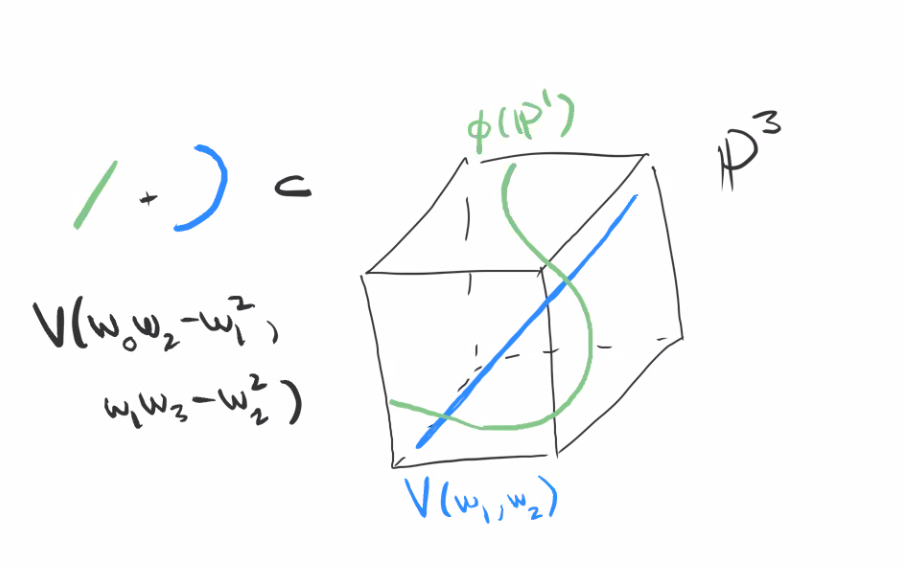
\includegraphics[width=3.64583in,height=\textheight]{figures/image_2020-11-24-10-16-35.png}
\caption{Image}
\end{figure}

This variety has two components: the twisted cubic, and a line. This
variety has degree 4, since any generic hyperplane intersects it at 4
points. Why? Pulling back a hyperplane yields a cubic, which generally
vanishes at three points in affine space.

\end{example}

\begin{remark}

\(\phi(\PP^1)\) is a nice example of a curve in \(\PP^3\) that can not
be cut out by two homogeneous polynomials.

\end{remark}

\begin{remark}

This is usually used to embed intersections like \(X\intersect V(f)\) to
\(X\intersect H\), exchanging a hypersurface section for a hyperplane
section. This is useful for induction:

\begin{enumerate}
\def\labelenumi{\arabic{enumi}.}
\tightlist
\item
  Prove for \(\PP^n\).
\item
  Induction: If it's true for \(X \subset\PP^n\), then it's true for
  \(X \intersect H\) for some hyperplane \(H \subset\PP^N\).
\end{enumerate}

This will prove it for any projective variety by taking
\(X = V(f_1, \cdots, f_n)\) and embedding.

\end{remark}

\hypertarget{chapter-10-smoothness}{%
\subsection{Chapter 10: Smoothness}\label{chapter-10-smoothness}}

Motivation: we want to distinguish between things like \(V(xy)\) and
\(V(xy-1)\).

\begin{figure}
\centering
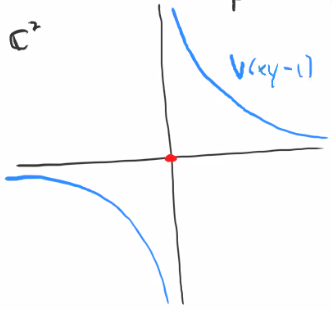
\includegraphics[width=3.64583in,height=\textheight]{figures/image_2020-11-24-10-31-47.png}
\caption{Image}
\end{figure}

Over \(\CC\), we can distinguish these: one is a complex manifold, and
the other is not. This means we want each point to have a neighborhood
biholomorphic to a disc.

\begin{definition}[Tangent Space]

Let \(a\in X\) be a point on a variety \(X\). Choose an affine open set
containing \(a\) and a chart such that \(a\) is the origin, then define
\begin{align*}  
T_a X \da V(f_1 \st f\in I(X))
,\end{align*} where \(f_1\) denotes the linear part of \(f\).

\begin{figure}
\centering
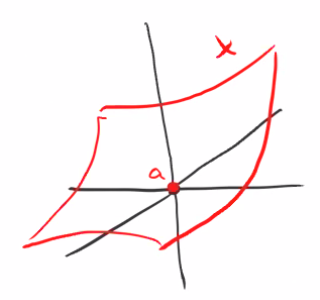
\includegraphics{figures/image_2020-11-24-10-38-10.png}
\caption{Image}
\end{figure}

\end{definition}

\begin{remark}

Since \(0=a\), any \(f\in I(X)\) has no constant term -- otherwise \(f\)
would not vanish at the origin.

\end{remark}

\begin{example}[?]

Consider \(T_{(1, 1)} V(xy-1)\). First translate \((1, 1)\) to the
origin, so
\(T_{(1, 1)} V(xy-1) = T_{(0, 0)} = V((x-1)(y-1) - 1) = T_{(0, 0)} V(xy-x-y) = V(-x-y)\).
On the other hand, \(T_{(0, 0)} V(xy) = V(0) = \CC^2\).

\begin{figure}
\centering
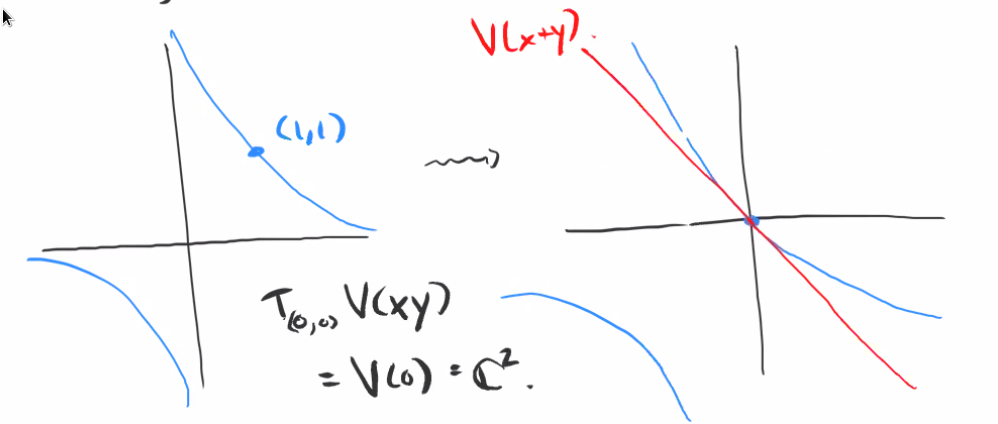
\includegraphics{figures/image_2020-11-24-10-41-13.png}
\caption{Image}
\end{figure}

\end{example}

\hypertarget{tuesday-december-01}{%
\section{Tuesday, December 01}\label{tuesday-december-01}}

Last time: we started discussing smoothness.

\begin{definition}[Tangent Space]

The \textbf{tangent space} \(T_p X\) of a variety \(X\) at a point
\(p\in X\) is defined as
\begin{align*}
V\qty{\ts{f_1 \st f\in I(U_i),\, U_i \ni p = 0 \text{ affine } }}
\end{align*} where \(f_1\) denotes the degree 1 part.

\begin{figure}
\centering
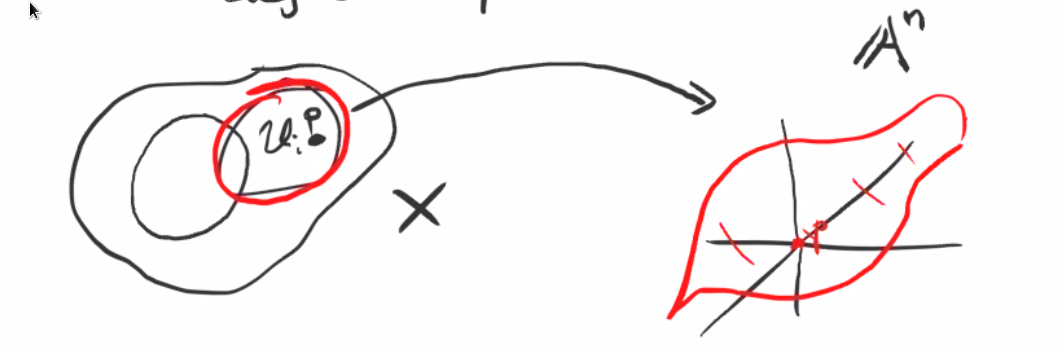
\includegraphics[width=3.64583in,height=\textheight]{figures/image_2020-12-01-09-40-28.png}
\caption{Image}
\end{figure}

\end{definition}

\begin{remark}

We've really only defined it for affine varieties and \(p=0\), but this
is a local definition. Note that this is also not a canonical
definition, since it depends on the affine chart \(U_i\).

\end{remark}

\begin{example}[?]

Consider \(T_0 V(xy) = V(f_1 \st f\in \gens{xy}) = V(0) = \AA^2\), since
every polynomial in this ideal has degree at least 2. Letting
\(X = V(xy)\), note that we could embed \(X\injects \AA^3\) as
\(X\cong V(xy, z)\). In this case we have
\(T_0 X = V(f_1 \st f\in \gens{xy, z}) = V(z) \cong \AA^2\). So we get a
vector space of a different dimension from this different affine
embedding, but \(\dim T_0 X\) is the same.

\end{example}

\begin{example}[?]

Let \(X = V_p(xy-z^2) \subset \PP^2\), which is a projective curve. What
is \(T_p X\) for \(p = [0:1:0]\)? Take an affine chart
\(\ts{y\neq 0} \intersect X\), noting that \(\ts{y\neq 0} \cong \AA^2\).
We could dehomogenize the ideal
\(\ro{\gens{xy-z^2}}{y=1} = \gens{x-z^2}\). Thus
\(X \intersect D(y) = V(x-z^2) \subset \AA^2\) and the point
\([0:1:0] \in X\) gives \((0, 0)\) in this affine chart. Then
\(T_p X = V(f_1 \st f\in \gens{x-z^2}) = V(x)\). Then \(f = (x-z^2)g\)
implies that \(f_1 = (xg)_1 = g_0 x\), the constant term of \(g\)
multiplied by \(x\), since \(z^2\) kills any degree 1 part of \(g\). So
\(T_p X\) is a line.

\end{example}

\begin{example}[?]

Take \(X\) to be the union of the coordinate axes in \(\AA^3\).

\begin{figure}
\centering
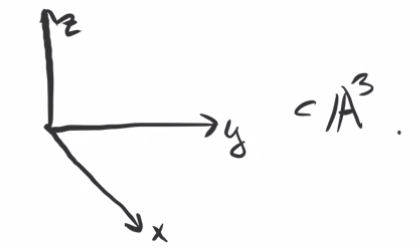
\includegraphics[width=3.64583in,height=\textheight]{figures/image_2020-12-01-09-54-30.png}
\caption{Image}
\end{figure}

Then \(I(X) = \gens{xy, yz, xz}\) and
\(T_0 X = V(f_1 \st f\in I(X)) = V(0) = \AA^3\), since the minimal
degree of any such polynomial is 2. Note that \(\dim X = 1\) but
\(\dim T_0 X = 3\)

\end{example}

\begin{example}[?]

Take \(Y = V(xy(x-y)) \subset \AA^2\). Then \(T_0 X = V(0) = \AA^2\):

\begin{figure}
\centering
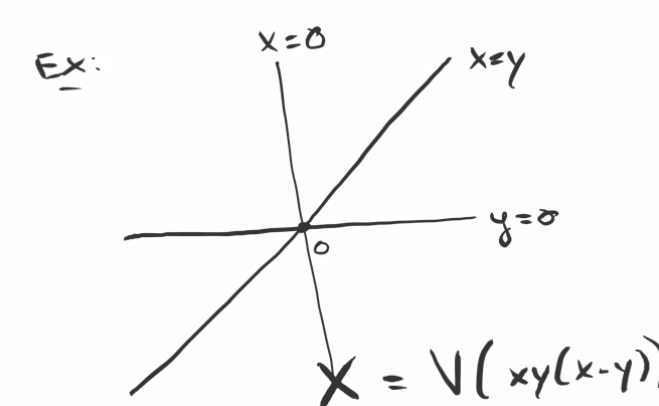
\includegraphics[width=3.64583in,height=\textheight]{figures/image_2020-12-01-09-59-06.png}
\caption{Image}
\end{figure}

\end{example}

\begin{remark}

Note that \(X\) and \(Y\) both consists of 3 copies of \(\AA^1\)
intersecting at a single point.

\begin{figure}
\centering
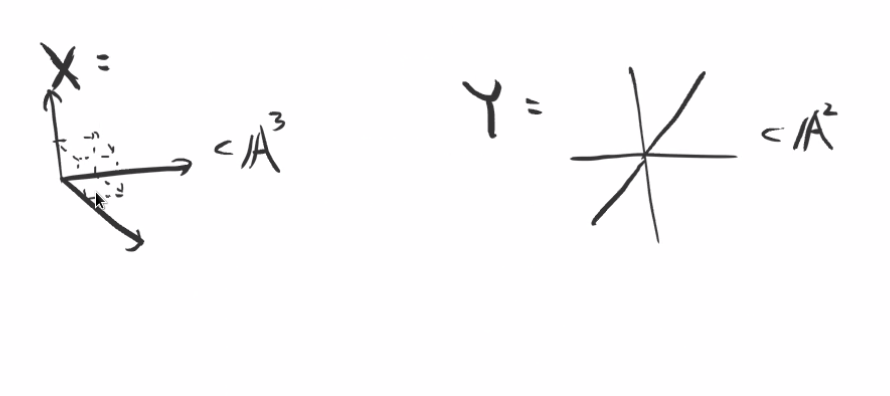
\includegraphics[width=3.64583in,height=\textheight]{figures/image_2020-12-01-10-01-58.png}
\caption{Image}
\end{figure}

Note that \(\dim T_0 X = 3\) but \(\dim T_0 Y = 3\), and interestingly
\(X\not\cong Y\) as affine varieties. There is a bijective morphism that
is not invertible.

\end{remark}

\begin{remark}

We will prove that \(\dim T_p X\) is invariant under choice of affine
embedding.

\end{remark}

\begin{example}[?]

How to compute \(T_{(1,0,0)} V(xy, yz, xz)\): first move \((1,0,0)\) to
the origin, yielding \(T_{(0,0,0)} V((x+1)y, yz, (x+1) z)\). This is a
different choice of affine embedding into \(\AA^3\) which sends
\((1,0,0) \mapsto (0,0,0)\). Taking the vanishing locus of linear parts,
it suffices to take the linear parts of the generators, which yields the
\(x\dash\)axis \(V(y, z)\), making the dimension of the tangent space 1.

\end{example}

\begin{lemma}[?]

Let \(X \subset\AA^n\) be an affine variety and let \(0 = p\in X\). Then
\begin{align*}
T_0(X)\dual \da \hom_k(T_0X, k) \cong I_X(p) / I_X(p)^2
\end{align*}

\end{lemma}

\begin{remark}

Note that the hom involves an affine embedding, but the quotient of
ideals does not. We know that the category of affine varieties is
equivalent to the category of reduced \(k\dash\)algebras, since the
points of \(X\) biject with the maximal ideals of the coordinate ring
\(A(X)\). \(I_X(p)\) is the maximal ideal in \(A(X)\) of regular
functions vanishing at \(p\).

\end{remark}

\begin{proof}[?]

Consider the map
\begin{align*}  
\phi: I_X(p) &\to T_0(X)\dual \\
\bar f &\mapsto \ro{f_1}{T_0(X)}
.\end{align*} E.g. given \(\bar x_1 - \bar x_2^2 \in A(X)\), we first
lift to \(x_1 - x_2^2 \in A(\AA^n)\), restrict to the linear part
\(x_1\), then restrict to \(T_0(X)\). Note that
\(I_X(p) = \gens{\bar x_1, \cdots, \bar x_n} \in k[x_1, \cdots, x_n]/I(X)\),
and we need to check that this well-defined since there is ambiguity in
choosing the above lift.

\begin{claim}

\(\phi\) is well-defined.

\end{claim}

Consider two lifts \(f, f'\) of
\(\bar f\in A(X) = k[x_1, \cdots, x_n]/I(X)\). Then \(f - f'\in I(X)\),
so \((f - f')_1 = f_1 - f_1'\) is the linear part of some element in
\(I(X)\). The definition of \(T_0(X)\) was the vanishing locus of linear
parts of elements in \(I(X)\), which contains \(f_1 - f_1'\), and thus
\(\ro{\qty{f_1 - f_1'} }{T_0(X)} = 0\). So \(f_1 = f_1'\) on \(T_0(X)\).

\begin{claim}

\(I_X(p)^2 \to 0\).

\end{claim}

We know \(I_X(p) = \gens{\bar x_1, \cdots, \bar x_n}\), and so
\(I_X(p)^2 = \gens{\bar x_i \bar x_j}\). Giving any
\(\bar f\in I_X(p)^2\), we can lift this to some
\(f\in \gens{x_i x_j}\), in which case \(f_1 = 0\).

So \(\phi\) descends to
\begin{align*}
\bar \phi: I_X(p) / I_X(p^2) &\to T_0(X)\dual \\
\end{align*}

\begin{claim}

\(\phi\) is injective and surjective.

\end{claim}

That \(\bar \phi\) is surjective follows from the fact that if
\(\bar x_1, \cdots, \bar x_n \in I_X(p)\), then the restrictions
\(\ro{x_1}{T_0X}, \cdots, \ro{x_n}{T_0X}\) are in \(\im \bar \phi\)
These elements generate \(T_0(X)\dual\), since \(T_0(X) \subset\AA^n\).
For injectivity, suppose \(\bar \phi(\bar f) = 0\), then
\(\ro{f_1}{T_0(X)} = 0\), so \(f_1\) is the linear part of some
\(f' \in I(X)\). Then \(f' \in I(X)\) and \(f, f'\) have the same linear
part \(f_1\), and \(f-f'\) has no linear part. Thus
\(f-f'\in \gens{x_i x_j}\), which implies that
\(\bar f - \bar f' \in I_P(X)^2\) and
\(\bar f \equiv \bar f' \in I_p(X) / I_p(X)^2\). But \(f' \equiv 0\)
since \(f'\in I(X)\).

\end{proof}

\begin{remark}

So for \(X\) an affine variety, the cotangent space has a more intrinsic
description, and we can recover the tangent space by dualizing:
\begin{align*}  
T_p(X) \da \qty{\mathfrak{m}_p/\mathfrak{m}_p^2 }\dual
\end{align*} where \(\mathfrak{m}_p = I_X(p)\) is the maximal ideal of
regular functions vanishing at \(p\). So how can we get rid of the word
affine? Given \(X\) any variety, we can define
\(T_p(X) \da \qty{\mathfrak{m}/\mathfrak{m}^2}\dual\) where
\(\mathfrak{m}\) is the maximal ideal of the local ring \(\OO_{X, p}\).
This allows us to work on affine patches and localize. Moreover, this
will be left invariant under the localization.

\end{remark}

\hypertarget{thursday-december-03}{%
\section{Thursday, December 03}\label{thursday-december-03}}

We showed last time that if \(X\) is an affine variety, then
\(T_p X = V\qty{f_1 \st f\in I(X)}\) for \(p = \vector 0 \in \AA^n\),
and we showed this is naturally isomorphic to
\(\qty{\mathfrak{m}_p /\mathfrak{m}_p^2}\). Then there was a claim that
generalizing this definition to an arbitrary variety \(X\) involved
taking \(\mathfrak{n}_p \leq \OO_{X, p}\), a maximal ideal in this local
ring of germs of regular functions, given by
\(\ts{(U, \phi) \st p\in U, \, \phi\in \OO_{X}(U)}\). In this case,
\(T_p = \qty{\mathfrak{n}_p/\mathfrak{n}_p^2}\). To prove this, it
suffices to show that
\(\mathfrak{m}_p/\mathfrak{m}_p^2 \cong \mathfrak{n}_p/\mathfrak{n}_p^2\).
Note that for any affine open \(U_i \ni p\), we have
\(\OO_{X, p} = \OO_{U_i, p}\).

When \(X\) is affine, we have
\(\OO_{X, p} = A(X)_{\mathfrak{m}_p} \da \ts{f/g \st f\in A(X), g\not\in \mathfrak{m}_p}/\sim\).
Note that this localization makes sense, since the complement of a
maximal ideal is multiplicatively closed since it is prime. The
equivalence relation was \(f/g = f'/g'\) if there exists an
\(s\not\in \mathfrak{m}_p\) such that \(s(fg' - f'g) = 0\). We want to
show that
\(\mathfrak{m}_p / \mathfrak{m}_p^2 = \mathfrak{m}_p A(X)_{\mathfrak{m_p}} / \mathfrak{m}_p A(X)_{\mathfrak{m_p}}^2\),
i.e.~this doesn't change when we localize. In other words, we want to
show that \(\mfm_p / \mfm_p^2 \cong S^{-1} \mfm_[ / (S^{-1} \mfm_p)^2\).

Let \(f\in S\) so \(f(p) \neq 0\). Then
\(\bar f\in A(X) / \mathfrak{m}_p \cong K\) is a nonzero element in a
field and thus invertible. Thus \(c\da 1/\bar f\) is an element of
\(K\units\), and for all \(g\in \mathfrak{m}_p\) we have
\(g/f \cong cg\) in \(\mathfrak{m}_p / \mathfrak{m}_p^2\). So
multiplying by elements of \(S\) is invertible in
\(\mathfrak{m}_p / \mathfrak{m}_p^2\). Thus
\(S^{-1} \qty{\mathfrak{m}_p / \mathfrak{m}_p^2} \cong \mathfrak{m}_p / \mathfrak{m}_p^2\),
where the LHS is isomorphic to
\(S^{-1} \mathfrak{m}_p / \qty{S\inv \mathfrak{m}_p^2}\).

\begin{definition}[Smooth/Regular Varieties]

A connected variety \(X\) is \textbf{smooth} (or \textbf{regular}) if
\(\dim T_p X = \dim X\) for all \(p\in X\). More generally, an arbitrary
(potentially disconnected) variety is smooth if every connected
component is smooth.

\end{definition}

\begin{example}[?]

\(\AA^n\) is smooth since \(T_p \AA^n = k^n\) for all points \(p\),
which has dimension \(n\).

\end{example}

\begin{example}[?]

\(\AA^n \disjoint \AA^{n-1}\) is also smooth since each connected
component is smooth.

\end{example}

\begin{definition}[Singular Varieties]

A variety that is not smooth is \textbf{singular} at \(p\) if
\(\dim T_p X \neq \dim X\).

\end{definition}

\begin{fact}

\(\dim T_p X\geq \dim X\) for \(X\) equidimensional, i.e.~every
component has the same dimension. This rules out counterexamples like
the following in \(\AA^3\):

\begin{figure}
\centering
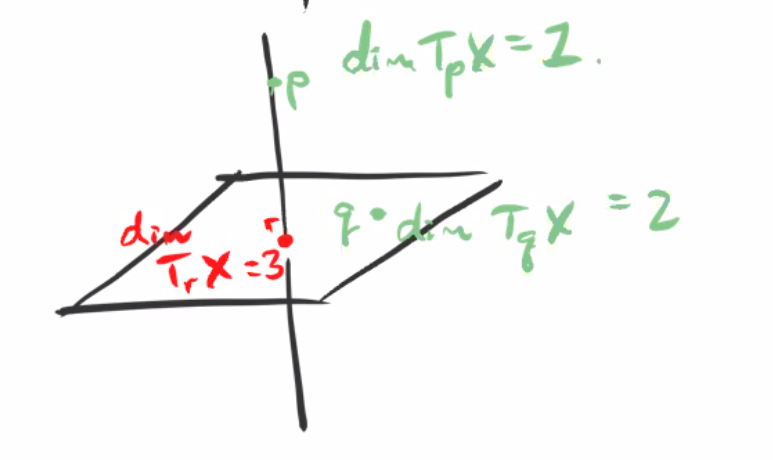
\includegraphics{figures/image_2020-12-03-10-05-17.png}
\caption{Union of Plane and Axis}
\end{figure}

\end{fact}

\begin{example}[?]

Consider \(X\da V(y^2 - x^3) \subset \AA^2\):

\begin{figure}
\centering
\includegraphics{figures/image_2020-12-03-10-07-39.png}
\caption{Image}
\end{figure}

Note that \(\dim T_0 X = 2\) is easy to see since it's equal to
\(V\qty{f_1 \st f\in \gens{y^2 - x^3}} = V(0) = k^2\). Thus \(p\neq 0\)
are smooth points and \(p=0\) is the unique singular point. So \(X\) is
not smooth, but \(X\smz\) is.

\end{example}

\begin{definition}[Regular Ring]

A local ring \(R\) over a field \(k\) is \textbf{regular} iff
\(\dim_k \mathfrak{m}/\mathfrak{m}^2 = \dim R\), the length of the
longest chain of prime ideals. Note that we'll add the additional
assumption that \(R/\mathfrak{m} \cong k\).

\end{definition}

\begin{remark}

A variety \(X\) is thus smooth iff
\(\dim_k \mathfrak{m}_p / \mathfrak{m}_p^2 = \dim_p X = \dim \OO_{X, p}\).

\end{remark}

\begin{theorem}[A hard theorem from commutative algebra (Auslander-Buchsbanm, 1940s)]

A regular local ring is a UFD.

\end{theorem}

\begin{corollary}[?]

Each connected component of a smooth variety is irreducible.

\end{corollary}

\begin{proof}[?]

If a connected component\(X\) is not irreducible, then there exists a
point \(p\in X\) such that \(\OO_{X, p}\) is not a domain, and thus a
nonzero pair \(f, g \in \OO_{X, p}\) such that \(fg=0\). These exist by
simply taking an indicator function on each component. So \(0\) doesn't
have a unique factorization. So \(\OO_{X, p}\) is not regular, and thus
\(\dim T_p X > \dim_p X\), which is a contradiction.

\end{proof}

\begin{remark}

How can we check if a variety \(X\) is smooth then? Just checking
dimensions from the definitions is difficult in general.

\end{remark}

\begin{proposition}[Jacobi Criterion]

Let \(p\in X\) an affine variety embedded in \(\AA^n\), and suppose
\(I(X) = \gens{f_1, \cdots, f_r}\). Then \(X\) is smooth at \(p\)
\(\iff\) the matrix \(\qty{\dd{f}{x_j}}\evalfrom_{p}\) has rank
\(n - \dim X\).

\end{proposition}

\begin{example}[?]

Is \(V(x^2 - y^2 - 1) \subset \AA^2\) smooth? We have
\(I(X) = \gens{f_1} \da \gens{x^2 - y^2 - 1}\), so let \(p\in X\). Then
consider the matrix
\begin{align*}  
\begin{bmatrix}
J \da 
\dd{f}{x} & \dd{f}{y} \\
\end{bmatrix} = 
\begin{bmatrix}
2x & -2y \\
\end{bmatrix}
.\end{align*} We want to show that at any \(p\in X\), we have
\(\rank(J) = 1\). This is true for \(p\neq (0, 0)\), but this is not a
point in \(X\).

\end{example}

\begin{example}[?]

Consider \(X \da V(y^2 - x^3 + x^2) \subset \AA^2\):

\begin{figure}
\centering
\includegraphics[width=3.64583in,height=\textheight]{figures/image_2020-12-03-10-32-44.png}
\caption{Image}
\end{figure}

Then \(I(X) = \gens{y^2 - x^3 + x^2} = \gens{f}\), and
\begin{align*}  
J = 
\begin{bmatrix}
2y & -3x^2 + 2x \\
\end{bmatrix}
.\end{align*} Then \(\rank(J) = 0\) at \(p = (0, 0)\), which is a point
in \(X\), so \(X\) is not smooth.

\end{example}

\begin{example}[?]

Consider \(X\da V(x^2 + y^2, 1+z^3) \subset\AA^3\), then
\(I(X) = \gens{x^2 + y^2, 1 + z^3} \gens{f, g}\) which is clearly a
radical ideal.

We then have
\begin{align*}  
J = 
\begin{bmatrix}
f_x & f_y & f_z \\
g_x & g_y & g_z \\
\end{bmatrix}
=
\begin{bmatrix}
2x & 2y & 0 \\
0 & 0 & 3z^2
\end{bmatrix}
,\end{align*} and thus
\begin{align*}  
\rank(J) = 
\begin{cases}
0 & x=y=z=0 \\
1 & x=y=0 \text{ xor } z=0 \\
2 & \text{else}.
\end{cases}
\end{align*}

We can check that \(\dim X = 1\) and \(\codim_{\AA^3} X = 3-1 = 2\), so
a point \((x,y,z) \in X\) is smooth iff \(\rank(J) = 2\). The singular
locus is where \(x=y=0\) and \(z= \zeta_6\) is any generator of the 6th
roots of unity, i.e.~\(\zeta_6, \zeta_6^3, \zeta_6^5\), along with the
point \(0\). Note that \(z=0\) is not a point on \(X\), since
\(1+z^3\neq 0\) in this case.

Thus the singular locus is
\(V(x^2 + y^2) = V((x+iy)(x-iy)) \intersect V(1+z^3)\), which results in
3 singular points after intersecting:

\begin{figure}
\centering
\includegraphics{figures/image_2020-12-03-10-42-21.png}
\caption{Image}
\end{figure}

Note that it doesn't matter that \(V(1+z^3)\) was intersected here, as
long as it's anything that intersects the \(z\dash\)axis nontrivially we
will still get something singular.

\end{example}

\hypertarget{misc-unsorted}{%
\section{Misc Unsorted}\label{misc-unsorted}}

\begin{figure}
\centering
\includegraphics{figures/image_2020-09-16-04-09-22.png}
\caption{Image}
\end{figure}

\section{Indices}
\listoftodos[List of Todos]
\newpage

% Hook into amsthm environments to list them.
\renewcommand{\listtheoremname}{Definitions}
\listoftheorems[ignoreall,show={definition}, numwidth=3.5em]

\renewcommand{\listtheoremname}{Theorems}
\listoftheorems[ignoreall,show={theorem,proposition}, numwidth=3.5em]

\renewcommand{\listtheoremname}{Exercises}
\listoftheorems[ignoreall,show={exercise}, numwidth=3.5em]

\listoffigures


\printbibliography[title=Bibliography]


\end{document}
